% Authors: Simon Geoffroy-Gagnon and Farhad Shokraneh
% Based on the Thesis by Rubana Bahar Priti
% Edit: 2020.04.16

\documentclass[12pt, TexShade, letterpaper]{report}
\usepackage[T1]{fontenc}
\usepackage[utf8]{inputenc}
\usepackage{palatino}
\usepackage{amsmath}
\usepackage{amssymb} 
\usepackage{graphicx}
\usepackage[labelfont=bf]{caption}
\usepackage{subcaption}
\usepackage{setspace}
%\captionsetup[table]{font = {stretch=1.35}}
%\captionsetup[figure]{font = {stretch=1.35}}
\captionsetup[table]{font = {stretch=1.0}}
\captionsetup[figure]{font = {stretch=1.0}}
\usepackage[margin=1in, headsep=1cm, bottom=5cm]{geometry}
%\usepackage[hidelinks]{hyperref}
%\usepackage[colorlinks=true]{hyperref}
\usepackage{hyperref}
%\newcommand{\MYhref}[3][blue]{\href{#2}{\color{#1}{#3}}}%
\usepackage{tabu}
%\usepackage{cite}
\usepackage[table]{xcolor}
%\usepackage{nomencl}
%\usepackage[nonumberlist,nogroupskip,xindy]{glossaries}
\usepackage{floatrow}
\usepackage{wrapfig}
\renewcommand{\baselinestretch}{2} 
\usepackage{fancyhdr}
\usepackage{lmodern}
\usepackage{titlesec}
\usepackage[natbib,style=numeric-comp,backend=biber,sorting=none,doi=false,isbn=false,url=false,eprint=false]{biblatex}

\usepackage{algorithm}
\usepackage{algpseudocode}
\usepackage{pdflscape}

\usepackage{times}

% Define some math operators
\DeclareMathOperator{\diag}{diag}
\DeclareMathOperator\supp{supp}

\definecolor{quotationcolour}{HTML}{F0F0F0}
\definecolor{quotationmarkcolour}{HTML}{1F3F81}

\addbibresource{phd_thesis.bib}

%%%%%%%%%%%%%%%%%%%
%
% FORMATTING HEADERS
%
%%%%%%%%%%%%%%%%%%%

% Format spacing around headers

%\titlespacing*{<command>}{<left>}{<before-sep>}{<after-sep>}
%\titleformat{<command>}[<shape>]{<format>}{<label>}{<sec>}{<before-code>}[<after-code>]

% Reduce gap between chapter header and chapter title
\titleformat{\chapter}
            [hang] %shape 
            {\vspace{-2cm}\bfseries\Large}
            {\thechapter}
            {20pt} % distance between number and title
            {} 
            []
            
% Make section titles a bit smaller than chapter titles
\titleformat{\section}
            [hang] %shape 
            {\bfseries\large}
            {\thesection}
            {20pt} % distance between number and title
            {} 
            []
            
\titleformat{\subsection}
            [hang] %shape 
            {\bfseries\normalsize}
            {\thesubsection}
            {20pt} % distance between number and title
            {} 
            []
            
\titlespacing*{\chapter}{0pt}{5.5ex plus 1ex minus .2ex}{0pt}

\titlespacing*{\section}
{0pt}{5.5ex plus 1ex minus .2ex}{0pt}

\titlespacing*{\subsection}
{0pt}{5.5ex plus 1ex minus .2ex}{0pt}

% Command to prevent \chapter from numbering chapters
% Otherwise you get stuff like "CHAPTER 3: Chapter one"
\makeatletter
\newcommand{\unchapter}[1]{%
  \begingroup
  \let\@makechapterhead\@gobble % make \@makechapterhead do nothing
  \chapter{#1}
  \endgroup
}
\makeatother

%\renewcommand{\chaptermark}[1]{\markboth{#1}{}} % Ensure List of Figs, ToC, and glossary are named in the header

% Custom headers for List of figures/tables (removes capitalization)
\renewcommand{\listfigurename}{List of figures}
\renewcommand{\listtablename}{List of tables}

% Overwrite the plain page style with a red line and page numbering
\fancypagestyle{plain}{%
	\fancyhf{} % clear all header and footer fields
	\fancyhead[R]{\textbf{\thepage}} % except the center
}

% Create the fancy page style header
\pagestyle{fancy}
\fancyhf{}
\lhead{\textbf{\nouppercase{\leftmark}}}
\chead{}
\rhead{\textbf{\thepage}}

\usepackage{xpatch}
\xpretocmd\headrule{\color{red}}{}{\PatchFailed}



%\author{\textcopyright Author, August, 2020}
%\date{}

% Don't break these acronyms up with hyphens

\hyphenation{DBSCAN}
\hyphenation{HDBSCAN}
\hyphenation{PCA}
\hyphenation{UMAP}

%\setcounter{chapter}{-1}

\begin{document}

% trying to get chapters to stop appearing as roman numerals in \ref
% jfc why is htis so hard
% \renewcommand{\thechapter}{\arabic{chapter}}

%%%%%%%%%%%%%%%%%%%
%
% TITLE PAGE
%
%%%%%%%%%%%%%%%%%%%

\begin{titlepage}
\begin{center}

%\vspace*{0.5cm}



% {\sf\bfseries\LARGE  Data Consistency in Scalable\\
% Multi-tier Architectures}


% {\rm\bfseries\LARGE  Data Consistency}
% \vspace{0.15cm}
% {\rm\bfseries\LARGE  in}
% \vspace{0.15cm}
% {\rm\bfseries\LARGE  Multi-tier and Cloud Applications}

{\sf\bfseries\LARGE  The entangled biobank: On the topology of high-dimensional human genetic data }

%\vspace{0.15cm}

%{\sf\bfseries\LARGE  goes here}

%\vspace{0.15cm}

%{\sf\bfseries\LARGE  and here}

%\vspace{1.8cm}

\vspace{1.5cm}

{\large Alexandr Diaz-Papkovich}

\vspace{1.5cm}

%\vspace{1cm}

%\vspace{1.4cm}

Quantitative Life Sciences, McGill University\\
Montr\'{e}al, Qu\'{e}bec, Canada\\
August 2023

\vspace{1.5cm}



% \date{\today}

%\vspace{1.4cm}

\begin{figure}[H]
\centering

\includegraphics[width=0.4\columnwidth]{mcgill_sig_red.jpg}
\end{figure}

\vspace{1.5cm}

\noindent
A thesis submitted to McGill University in partial\\
fulfillment of the requirements of the degree of\\
Doctor of Philosophy


\vspace{1.4cm}

{\small \copyright Alexandr Diaz-Papkovich, 2023}


\end{center}
\end{titlepage}







\begin{spacing}{1}
 % Start of table of contents
\tableofcontents\thispagestyle{plain}
\end{spacing}{1}

% Set page numbering to roman
\cleardoublepage
\setcounter{page}{1}\renewcommand{\thepage}{\roman{page}}	

%%%%%%%%%%%%%%%%%%%
%
% ABSTRACT
%
%%%%%%%%%%%%%%%%%%%

\chapter*{Abstract}\markboth{Abstract}{}
	\label{chap:engAbstract}
	\addcontentsline{toc}{chapter}{Abstract}  
	Oh god!

%%%%%%%%%%%%%%%%%%%
%
% FRENCH ABSTRACT
%
%%%%%%%%%%%%%%%%%%%

\chapter*{Résumé}\markboth{Résumé}{}
	\label{chap:frAbstract}
		\addcontentsline{toc}{chapter}{Résumé}  
		Avec les progrès de la génomique, les biobanques sont en plein essor. Contenant les données génétiques de millions d'individus, les biobanques sont de riches dépôts, utilisés régulièrement et stimulant la découverte scientifique. Le génome humain s'étend sur environ trois milliards de paires de bases, ce qui fait de l'étude des données génétiques à grande échelle une tâche dans un espace de grande dimension. L'échelle même du problème est un défi, tout comme la complexité de la diversité génétique humaine. Grâce à de nouvelles méthodes d'analyse topologique des données, nous sommes en mesure de réduire la dimensionnalité de ces ensembles massifs de données tout en préservant d'importantes quantités d'informations à l'aide d'une méthodologie traçable à l'échelle de la biobanque.

Dans le cadre de cette recherche, nous appliquons «~uniform manifold approximation and projection~» (UMAP), une forme de la réduction de la dimensionnalité non linéaire, et HDBSCAN, un algorithme de regroupement basé sur la densité des données, à plusieurs biobanques de données génétiques humaines. Nous utilisons UMAP et HDBSCAN pour étudier la structure de la population, le phénomène dans lequel la variation génétique n'est pas aléatoire et est corrélée à des facteurs tels que la géographie, l'histoire démographique, la migration et la structure sociale. Nous développons une méthodologie qui nous permet de visualiser les données génétiques, d'identifier la structure de la variation génétique allant d'une poignée à des centaines de milliers d'individus. Nous découvrons des relations subtiles entre la génétique, l'histoire, la géographie et la distribution des phénotypes.

%%%%%%%%%%%%%%%%%%%
%
% ACKNOWLEDGEMENTS
%
%%%%%%%%%%%%%%%%%%%

\chapter*{Acknowledgements}\markboth{Acknowledgements}{}
	\label{chap:acknowledgments}
			\addcontentsline{toc}{chapter}{Acknowledgements}  
	This thesis would not have been possible without my many communities, nor without the contributions of those who donated their data to further our understanding of genetics.

I would like to thank Simon Gravel for his guidance and mentorship and his balance of energetic curiosity with scientific scepticism, and the members of my supervisory committee, Nada Jabado and Ryan Hernandez. I would also like to thank Celia Greenwood, the director of QLS, and Alex DeGuise, the co-ordinator, for all of their hard work.

Thank you to my QLS cohort for grinding it out with me: Myriah Haggard, Matt D'Iorio, Jeffrey Hyacinthe, Yixiao Zheng, and Sara Zapata-Marin; to Selin Jessa, for sending me down the rabbit hole; to Noor Al-Sharif and Jake Vogel, for making Montreal feel like home; to my Thomson House Trivia crew: Matt, Barbara, Hector, Gerardo, JT, Val, and Rozzy, for being champions; to the Gravel lab, especially my desk-mate Chief Ben-Eghan who always made me laugh.

Thank you to my friends in my other homes. Those in Ottawa: Dylan, Leo, Julie, Ashley, Shane, Isaac, Amy, thanks for always wanting to see me when I was in town. To my friends in KW: Jake, Kayla, Warren, Kaitlin, Jon, Steph, Derek, Christina, Dave, Rebecca, Tyler, and Aine, thanks for entertaining my rants on Slack---may your broods grow belligerent and numerous.

Thank you to my loved ones: to Melissa, for exploring the forests and rivers with me; to my brother, Andrew, and my mother, Marina, for carrying me when I stumbled; and lastly to my father, Andr\'{e}s, who started this marathon with me so long ago---the finish line is finally in sight, and I can hear you cheering.

\pagebreak
\hspace{0pt}
\vfill

\begin{center}
%\begin{minipage}{.7\linewidth}
In memory of Andr\'{e}s Carlos D\'{i}az Bravo.
%\end{minipage}
\end{center}

\vfill
\hspace{0pt}
\pagebreak


%%%%%%%%%%%%%%%%%%%
%
% CONTRIBUTION TO KNOWLEDGE
%
%%%%%%%%%%%%%%%%%%%

\chapter*{Contribution to original knowledge}\markboth{Contribution to original knowledge}{}
	\label{chap:knowledge}
			\addcontentsline{toc}{chapter}{Contribution to original knowledge}  
	The works presented in this thesis establish novel methodologies for dimensionality reduction, clustering, and visualization in population genetics with possible extensions to genomics at large. We explore applications of UMAP, a nonlinear dimensionality-reduction method, and HDBSCAN($\hat{\epsilon}$), a density-based clustering algorithm. The two methods form the basis of our topological data analysis. The approach is tractable, easy-to-implement, and fits in the paradigm of exploratory-confirmatory analysis of biobank data, particularly for large and complex cohorts.

In \hyperref[chap:chapter1]{Chapter~1} we apply UMAP to population genetic data for the first time. We establish that it efficiently reveals fine-scale population structure in biobanks and use it in data visualization in 2- and 3-dimensions. These visualizations correlate with a number of phenotypic, geographic, and socio-demographic measures, and often appear as clusters. As UMAP became popular in the field, in \hyperref[chap:chapter2]{Chapter~2} we review its use in population genetics and provide insights on its optimal use and potential downstream applications.

Finally, in \hyperref[chap:chapter3]{Chapter~3} we address algorithmic clustering of UMAP results. We apply HDBSCAN($\hat{\epsilon}$) to UMAP data in $3$ to $5$ dimensions and use it to stratify biobank data. We discover clusters of structure in genetic data and leverage them to study demographic histories of populations in biobanks, polygenic score transferability, phenotype distributions, identify potentially influential alleles, and its use in quality control.

%%%%%%%%%%%%%%%%%%%
%
% CONTRIBUTIONS OF AUTHORS
%
%%%%%%%%%%%%%%%%%%%

\chapter*{Contributions of authors}\markboth{Contributions of authors}{}
	\label{chap:authors}
			\addcontentsline{toc}{chapter}{Contributions of authors}  
	\section*{Chapter 2}
\begin{itemize}
\item \textbf{Alex Diaz-Papkovich}: Conceptualization, data curation, formal analysis, investigation, methodology, software, visualization, writing -- original draft, writing -- review \& editing 
\item \textbf{Luke Anderson-Trocm\'{e}}: Visualization
\item \textbf{Chief Ben-Eghan}: Data curation
\item \textbf{Simon Gravel}: Supervision, writing -- review \& editing
\end{itemize}

Acknowledgements: Audrey Grant, Ryan Hernandez, Jose Sergio Hleap, Mark Lathrop, Dominic Nelson, Markus Munter, Stephen Sawcer, Melissa Spear, and Dara Torgerson for useful discussions about science, programming, and data access; David Poznik, Liz Babalola, and Adam Auton for discussing findings in the 1KGP; Selin Jessa for introducing us to UMAP

\section*{Chapter 3}

\begin{itemize}
\item \textbf{Alex Diaz-Papkovich}: Conceptualization, data curation, formal analysis, investigation, methodology, software, visualization, writing -- original draft, writing -- review \& editing
\item \textbf{Luke Anderson-Trocm\'{e}}: Visualization, data curation
\item \textbf{Simon Gravel}: Supervision, writing -- review \& editing
\end{itemize}

\section*{Chapter 4}
\begin{itemize}
\item \textbf{Alex Diaz-Papkovich}: Conceptualization, data curation, formal analysis, investigation, methodology, software, visualization, writing -- original draft, writing -- review \& editing
\item \textbf{Shadi Zabad}: Software, data curation
\item \textbf{Chief Ben-Eghan}: Data curation
\item \textbf{Luke Anderson-Trocm\'{e}}: Visualization, data curation
\item \textbf{Georgette Femerling}: Data curation
\item \textbf{Vikram Nathan}: Methods testing
\item \textbf{Jenisha Patel}: Methods testing
\item \textbf{Simon Gravel}: Supervision, writing -- review \& editing
\end{itemize}

Acknowledgements: Claude Bh\'{e}rer, Melissa Spear, and Paul Verdu for scientific discussion.

%%%%%%%%%%%%%%%%%%%
%
% LIST OF ACRONYMS
%
%%%%%%%%%%%%%%%%%%%

\chapter*{List of abbreviations}\markboth{List of abbreviations}{}
	\label{chap:abbrevs}
			\addcontentsline{toc}{chapter}{List of abbreviations}  
	%\addcontentsline{toc}{chapter}{Acronyms}
\scriptsize

\begin{table}[!h]
\vspace{-2.0cm}
\hspace{1.0cm}
\begin{tabular}{l l r}

\textsc{PCA}  & Principal component analysis \\ [1ex]
\textsc{UMAP}  &  Uniform manifold approximation and projection \\ [1ex]



\end{tabular}
\end{table}












%%%%%%%%%%%%%%%%%%%
%
% LIST OF FIGURES
%
%%%%%%%%%%%%%%%%%%%

\cleardoublepage
\listoffigures
\addcontentsline{toc}{chapter}{\listfigurename}

%%%%%%%%%%%%%%%%%%%
%
% LIST OF TABLES
%
%%%%%%%%%%%%%%%%%%%

\cleardoublepage	
\listoftables
\addcontentsline{toc}{chapter}{\listtablename}

\cleardoublepage

% Pre-amble done, time for Actual Content
% restart page numbers at one, now in arabic style
\setcounter{page}{1}\renewcommand{\thepage}{\arabic{page}}	

%%%%%%%%%%%%%%%%%%%
%
% INTRO AND LIT REVIEW
%
%%%%%%%%%%%%%%%%%%%

\begin{refsection}
\part{Introduction and literature review}
\label{part:intro}

\pagebreak
\hspace{0pt}
\vfill

\begin{center}
\begin{quote} 
\begin{singlespace}
\textit{
\textbf{Fry:} Here you are in the year 3000 or so, yet you just sit around like it's the boring time I came from.\\
\textbf{Professor Farnsworth:} Boring?! Wasn't that the period when they cracked the human genome, and boy bands roamed the earth? \\
---Futurama, S03E11 (2001)}
\end{singlespace}
\end{quote}
\end{center}

\vfill
\hspace{0pt}
\pagebreak

\unchapter{Introduction}
\chapter*{Chapter 1: Introduction}
%\begin{figure}
%  \includegraphics[width=0.25\linewidth]{main_figures/test_figure.png}
%  \caption{A figure.}
%  \label{fig:test_fig}
%\end{figure}
%
%\newpage

In 2001, the first analyses of the draft human genome were published in sister papers in \textit{Nature} and \textit{Science}. The Human Genome Project had been budgeted US\$$3$~billion in 1990; by 2020 the cost of sequencing a human genome had dropped to US\$$1,000$, and a relative paucity of data had given way to abundance\citep{gibbs_human_2020}. Biobanks with data from tens or hundreds of thousands of individuals are becoming commonplace.

Every genome carries both the stories of its ancestors and the basic programming of its bearer's physiology. By identifying patterns across many genomes and their associated data, we can infer their histories and study distributions of biomedical traits. The complexities of human history and society, to say nothing of the complexities of biology itself, ensure that this is a non-trivial task.

With each genome spanning $3$~billion base pairs, any mathematical investigation is high-dimensional. This thesis explores applications of dimensionality reduction to population genetic data, focusing on uniform manifold approximation and projection (UMAP), a method of topological data analysis.

This thesis is organized into three chapters that have been published as stand-alone manuscripts. In \hyperref[chap:chapter1]{Chapter~1} we apply UMAP to human genetic data for the first time. We use genotype data from three biobanks, generating visualizations and observing patterns in relatedness, demographic histories, geographic distribution, phenotype distributions, and other phenomena. In \hyperref[chap:chapter2]{Chapter~2} we review the applications of UMAP in other human genetic datasets, such as different biobanks or other types of genetic data (e.g. structural variants). Finally, in \hyperref[chap:chapter3]{Chapter~3} we formalize a methodology to use UMAP in higher dimensions ($n \ge 3$) and extract clusters.

% high-level concepts?
% shape of data
% population structure
% complexity and interrelatedness

\section{Genetic diversity}

The human genome spans over $3$~billion nucleobase pairs organized across $23$ pairs of chromosomes---$22$ pairs of autosomes and one pair of sex chromosomes---with some DNA present in mitochondria (mtDNA). The human genome is diploid (i.e. paired) with one set of chromosomes coming from each parent via their gametes; these chromosomes are created through the process of meiotic recombination, in which the chromosomes of grandparents are aligned, cross over, and recombine. Along with mutation, recombination generates diversity. Approximately $99.9\%$ of DNA shared between humans is identical, with genetic variants (alleles) arising through mutations. Single nucleotide polymorphisms (SNPs) are relatively common variants, usually defined as having a frequency above $1\%$.

Variants that lie along the same chromosome and are not broken up through recombination are co-inherited and are linked. The block of allelic states along a DNA molecule is referred to as a haplotype, and when the same variants exist between two individuals, they are said to be identical by state (IBS). If the shared variant is inherited from a common ancestor without recombination, they are also said to be identical by descent (IBD); alleles that are IBS are typically IBD, with rare exceptions. Alleles that are physically closer are more likely to be inherited together, and those that appear together more often than expected at random are said to be in linkage disequilibrium (LD). Combining two haplotypes gives a diploid genotype, and assuming free recombination, the theoretical maximum number of possible unique haplotypes is $2^L$, where $L$ is the number of SNPs.

Recombination is not uniformly random. DNA that does not lie in the pseudoautosomal regions (PAR1 and PAR2) of the Y chromosome, as well as mtDNA, does not recombine\citep{jobling_human_2013}. Recombination rates also vary within chromosomes with certain regions known to be hotspots\citep{altemose_map_2017}. Germline mutations may result from copying errors during replication or from spontaneous errors from DNA’s instability or external factors like UV radiation. Whole genome sequencing pedigree-based studies estimate the overall mutation rate at about $10^{-8}$ per base pair per generation, though this rate may vary depending on the mechanistic source of the mutation\citep{segurel_determinants_2014}.

\subsection{Population structure}

% what does structure *look* like?

In aggregate, patterns will form in the distributions of alleles; these patterns are known as population structure. Though genetic diversity is random in principle, the distributions of variants are shaped by environments and events. Phenomena like migrations, population bottlenecks, and non-random mating contribute to the distribution of alleles.

Why is genetic variation not fully random? How do we measure it? What are the processes that we know of? What are some historical examples?

\subsection{Measures of population structure}

\subsubsection{Hardy-Weinberg Equilibrium}

\subsubsection{Fixation index}

\subsection{Ancestry and admixture}

\section{Exploratory data analysis}

Traditional statistical analyses of biological data follow the recommendations of R.A. Fisher in the 1930s\citep{holmes_modern_2019}. They have a linear structure: beginning with a biological question, an investigator forms a hypothesis and an associated null ($H_0$), designs an experiment, collects data, tests $H_0$ with a p-value, and formulates a conclusion. Beginning in the 1970s, statistician John W. Tukey proposed the alternative framework of exploratory data analysis (EDA)\citep{tukey_1977,hoaglin_john_2003}. This approach is iterative and instead begins with the data: we visualize it, understand it, and use it to inform what sort of analysis to use in an accompanying confirmatory data analysis. The two contrasting approaches are schematized in Figure~\ref{fig:paradigms}.

\begin{figure}[h!]
\centering
\begin{subfigure}{0.3\textwidth}
    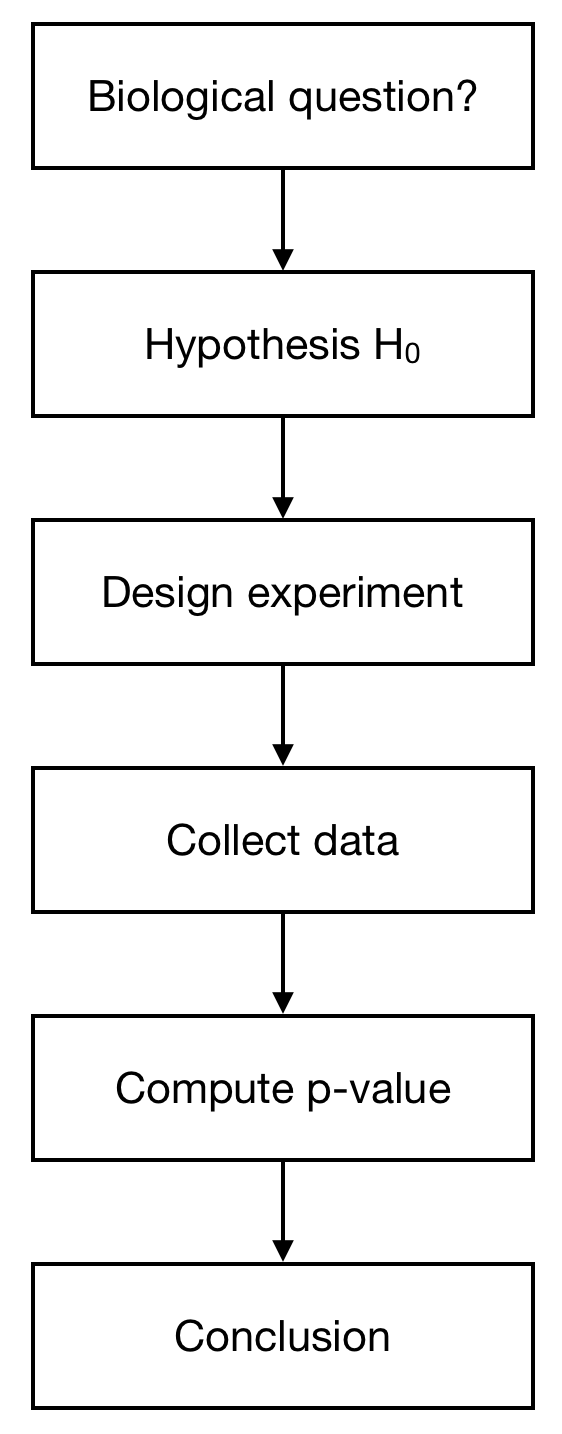
\includegraphics[height=0.5\textheight]{main_figures/intro/fisher_paradigm.png}
    \caption{Fisher's paradigm.}
    \label{fig:fisher}
\end{subfigure}
\hfill
\begin{subfigure}{0.65\textwidth}
    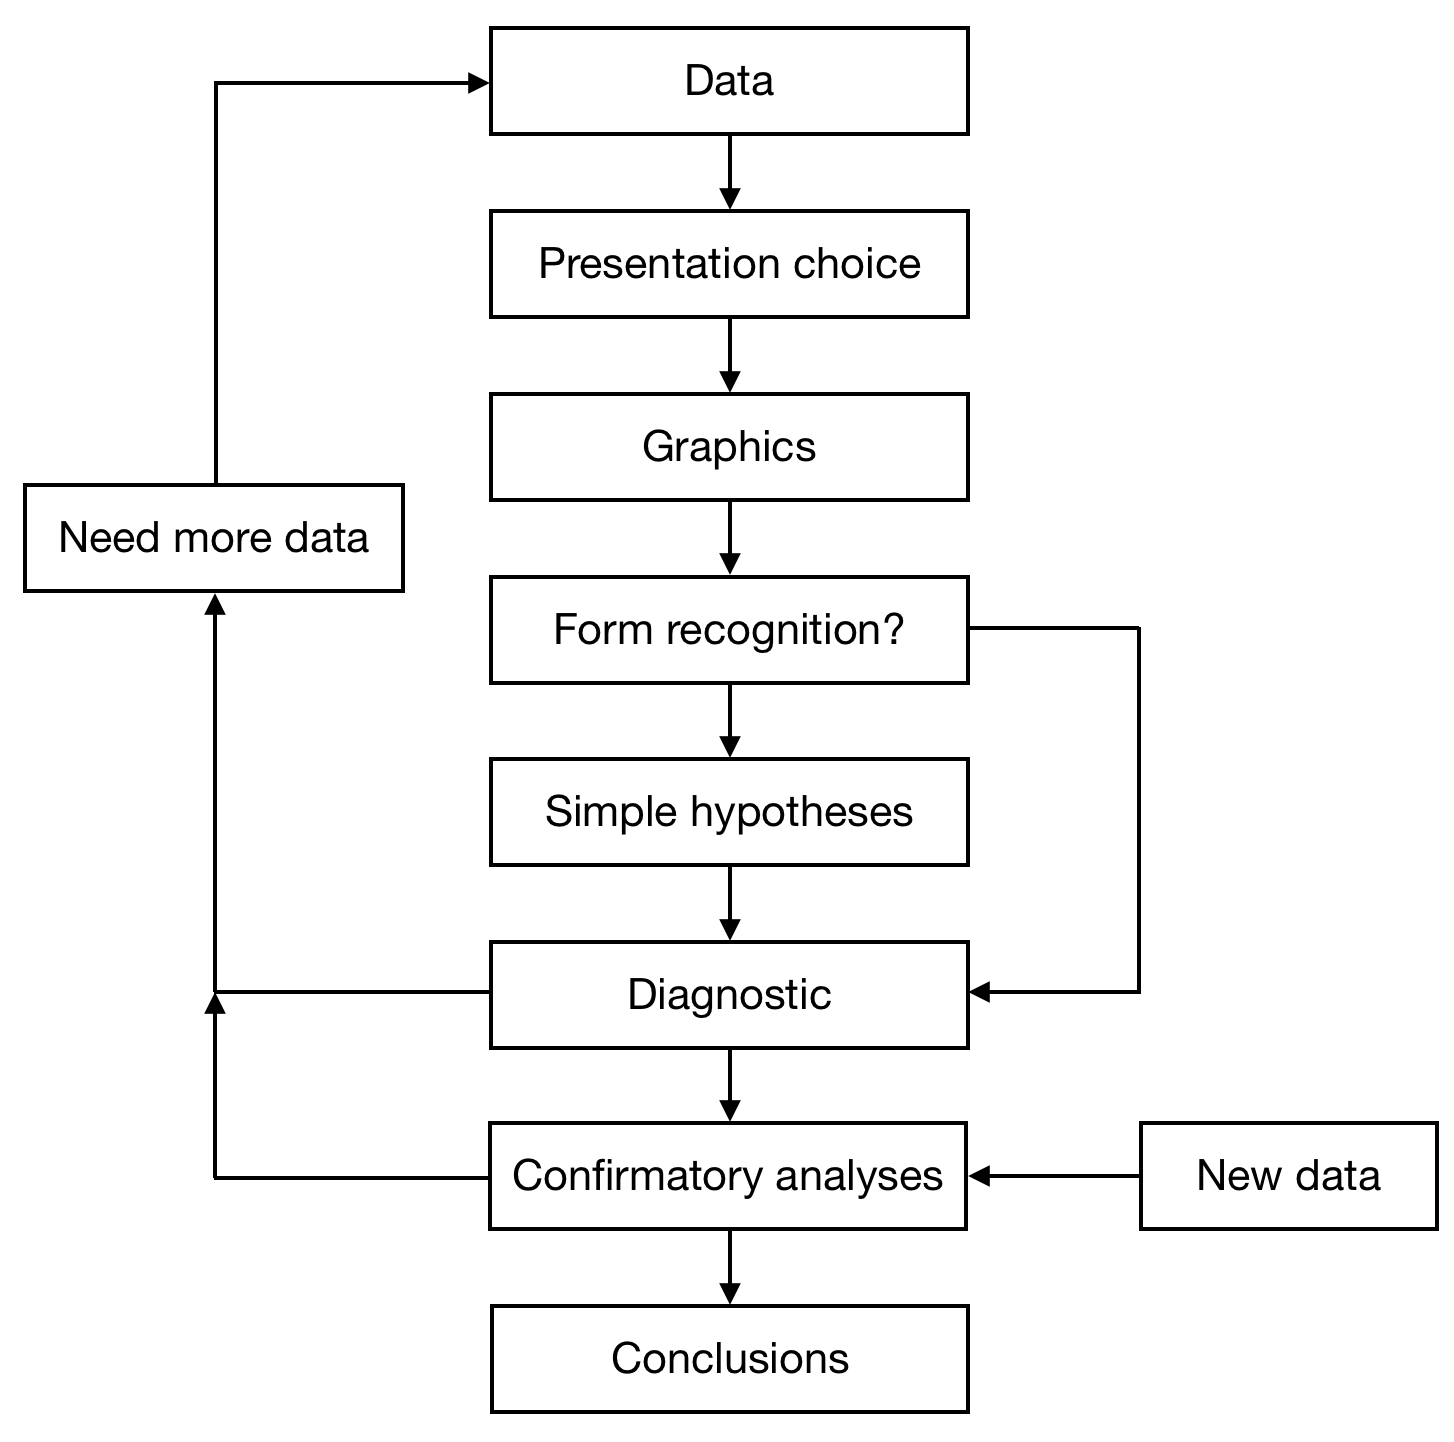
\includegraphics[height=0.5\textheight]{main_figures/intro/tukey_paradigm.png}
    \caption{Tukey's paradigm.}
    \label{fig:tukey}
\end{subfigure}
\caption{\textbf{Contrasting Fisher's paradigm with Tukey's paradigm in biology.} Fisher's paradigm (left) takes a sequential approach to data analysis, beginning with a well-defined question and strong assumptions. Tukey's paradigm (right) is iterative, beginning with the data, emphasizing exploratory analysis through visualization, and complemented by confirmatory analyses that are robust and do not rely on complex assumptions\citep{holmes_modern_2019}.}
\label{fig:paradigms}
\end{figure}

Writing in 1980, Tukey emphasized that science neither begins with a tidy question nor ends with a tidy answer\citep{tukey_we_1980}. This is especially true in modern biology. Statistical questions from the 1930s typically had a few parameters $p$ with a manageable sample size $N$ (where $N > p$), and the people posing questions were involved in data collection. Today we sit at the opposite extreme; it is not unusual for data to have $p >> N$ with the two values differing by orders of magnitude. When studying a biobank, we may have several thousand individuals and several hundred thousand genetic markers. Generally, the people investigating data have not collected it. These factors make Tukey's paradigm much better suited to our analytical needs\citep{holmes_modern_2019}. 

\subsection{Dimensionality reduction}

In Figure~\ref{fig:tukey}, the iterative process includes presentation choices, graphics, and form recognition. This provokes a natural question: what approaches ought we use here? With genomic data comes the ``curse of dimensionality'': though we have many dimensions to our data, the signal is sparse and many methods are computationally intractable. This motivates dimensionality reduction---we wish to reduce our data to a relatively low number of dimensions, ideally preserving important characteristics of the data. Given a satisfactory representation of the data set, we can visualize it.

\subsubsection{Principal component analysis}
Principal components analysis (PCA) is a non-parametric linear transformation that projects data onto a series of orthogonal axes based on a linear combination of the original data. The axes are generated and ordered according to their eigenvalues, and the ratio of each axis' corresponding eigenvalue to the sum of all eigenvalues represents the variance explained by that axis. PCA fits an ellipsoid around the data in high dimensions and the axes of that ellipsoid are the principal components. By only selecting the largest axes---corresponding to the most explained variance --- we can reduce the dimensionality of our data while preserving significant explanatory value. We can also interpret our dimensionally reduced data in terms of how much of the overall variance it explains. Principal components are calculated through eigendecomposition of the covariance matrix; a derivation for genotype data is given in \hyperref[appendix:AppendixA]{Appendix~A}. A detailed examination of PCA in the context of population genetics can be found in \citep{mcvean_genealogical_2009}. 

PCA has seen wide application in population genetics. The top PCs often reflect isolation-by-distance and are used for visualization (e.g. within Europe\citep{novembre2008europe}). However, using them for visualization requires selecting which components to examine and is limited to $2$ or $3$ dimensions; if there is signal beyond the first few PCs, it may go unnoticed. We expand on this in \hyperref[chap:chapter1]{Chapter~1}.

They are also used to correct for population structure in genome-wide association studies (GWAS) by their inclusion as covariates in models\cite{price_principal_2006}. There are varying rules-of-thumb on how many PCs to include in a model, such as using the top $10$, looking for an ``elbow'' in the scree plot, or testing for eigenvalue significance in the Wishart distribution; however, these are merely conventions. We explore the impact of PC adjustment for phenotypes in biobanks in \hyperref[chap:chapter3]{Chapter~3}. 

\subsection{Topological data analysis}

% Note to self: Rewrite this in terms of popgen challenges
% can maybe get philosophical here
We are often interested in learning about our data in to understand its large-scale structure, e.g., identifying different cell types or related individuals. Though we have some definitions of distances, we are interested in notions of \textit{similarity} or \textit{nearness}. Topology provides the mathematical machinery for ideas rooted in qualitative geometry\citep{carlsson_topology_2009}. Topological data analysis (TDA) is a set of statistical methods that uses ideas of shape and connectivity to study data\citep{wasserman_topological_2018}. We will focus on applications of manifold learning, non-linear dimensionality reduction, and density clustering.

TDA assumes that we observe a sample $X_1, \dots, X_n \sim P$ with $P$ supported on some set $\supp(P) = \mathcal{X} \subseteq \mathbb{R}^d$. 
In the simplest case of manifold learning, we suppose that $P$ is actually supported on some set $S$ with dimension $r$, where $r < d$ and $S$ is a smooth and compact manifold, and we may estimate $S$. PCA is a special case of linear manifold learning where data are assumed to lie on or near an affine subspace\citep{wasserman_topological_2018}. In cases where there is local nonlinear structure (such as clustering), nonlinear methods of manifold learning are more useful\cite{izenman_introduction_2012}.

In population genetics, we observe samples from, e.g., the distributions of genotypes.

\subsection{\texorpdfstring{$\mathbf{t}$}{f}-distributed stochastic neighbour embedding}
% the {f} here doesn't do anything, but we need a text character for compilation

$t$-distributed stochastic neighbour embedding ($t$-SNE) is a method of manifold learning used for visualization that was developed in 2008\citep{maaten_visualizing_2008}. By then, several methods existed to approximate the local structure of manifolds, but they suffered from the ``crowding problem''---in an attempt to preserve local distances between points, many of them are crunched together, eliminating the gaps between clusters. $t$-SNE addressed this by introducing a repulsion force between points, modelling pairwise distances between points $i$ and $j$ as a $t$-distributed random variable with $1$ degree of freedom (equivalent to a Cauchy distribution). The distances are modelled as probabilities:

$$q_{ij} = \frac{(1 + ||y_{i} - y_{j}||^{2})^{-1}}{\sum_{k \neq l}(1 + ||y_{k} - y_{l}||^{2})^{-1}}$$

This choice was largely ad-hoc and was later found to work because it optimized structure at the local scale (i.e. within clusters) as well as causing points to repel each other (i.e. causing clusters to separate)\citep{carreira-perpinan_elastic_2010}. This repulsion allowed $t$-SNE and related methods to preserve topology\citep{wasserman_topological_2018}. Because $t$-SNE can only reduce data to $2$ or $3$ dimensions, it was not recommended as a general purpose dimensionality reduction algorithm\citep{maaten_visualizing_2008}. It saw considerable use in visualization in single-cell genomics\citep{kobak_art_2019}, but its application in population genetics was limited (e.g. \citep{li_application_2017}). We provide details on $t$-SNE's performance in population genetics in \hyperref[chap:chapter1]{Chapter~1}.

\subsection{Uniform manifold approximation and projection}

Uniform manifold approximation and projection (UMAP) is a general purpose dimensionality reduction method rooted in algebraic topology and Riemannian geometry that was introduced in 2018\citep{mcinnes_umap_2020}. Unlike the more heuristic approach of $t$-SNE, the motivation behind UMAP is to represent the high-dimensional topology of data in low dimensional space. We will briefly outline the intuition underlying UMAP; details on the topology and theoretical justifications are available in \citep{mcinnes_umap_2020}, with a more applied explanation available in online documentation\citep{mcinnes_umapdoc_2018}.

We assume our data $X = \{X_{1}, \dots, X_{n}\}$ lay on some manifold and are uniformly distributed. For this assumption to hold, each point $X_{i}$ has its own custom distance, defined as the normalized distance to its $k\textsuperscript{th}$ nearest neighbour; thus, each $X_{i}$ has its own metric space, and is the centre of a unit ball that extends to the $k\textsuperscript{th}$ nearest neighbour. If we represent this as a graph, each $X_i$ is a point with edges to its $k$ neighbours, where the distances represent the edge weights. If we represent this as a simplicial complex, a point is a $0$-simplex and an edge is a $1$-simplex; according to theory, this simplicial complex forms an open cover of the underlying topological space. As the edge weights are between $0$ and $1$, we may also interpret the values as the belongingness to an open cover rather than a binary ``yes'' or ``no'' value---a fuzzy topological cover. To harmonize the respective edge weights $a, b$ from points $X_{a}$ to $X_{b}$ (since each point has its own local metric), UMAP defines the combined weight as $a + b - a \times b$, interpreted as the probability that an edge weight between $X_{a}$ and $X_{b}$ exists. The final high-dimensional product is a fuzzy simplicial complex, which can be represented as a weighted graph, and is a fuzzy topological representation of the data.

For the low-dimensional representation, we carry out the same process of building a fuzzy topological representation. However, rather than using a locally-varying metric, we assume that our data will lay on a low-dimensional Euclidean space, and we specify a minimum distance we wish to have between our points in this space. The algorithm then minimizes the cross-entropy function between the high- and low-dimensional representations. If $E$ is the set of all possible $1$-simplices, $w_{h}(e)$ is the weight of edge $e$ in the high-dimensional space and $w_{l}(e)$ the low-dimensional space, we minimize:

$$ \sum_{e \in E} w_{h}(e) \log{\left(\frac{w_{h}(e)}{w_{l}(e)}\right)} + (1 - w_{h}(e)) \log{\left(\frac{1 - w_{h}(e)}{1 - w_{l}(e)}\right)} $$

Though the machinery seems roundabout in its derivation, it allows for reduction of data to an arbitrary number of dimensions and for topological interpretations. The value of $k$ defines the scale of the topology we wish to approximate, with lower values being more local and finer-scale and higher values approximating broader manifold structure. Each chapter of this thesis discusses the uses and parametrizations of UMAP in population genetics: briefly, lower values of $k$ approximate closer relationships, e.g., at a structure as fine-scale as families; higher values of minimum distance facilitate visualization, while lower values facilitate algorithmic cluster detection.

UMAP is the core method of this thesis. In \hyperref[chap:chapter1]{Chapter~1}, we use UMAP in population genetics for the first time, exploring its potential applications thoroughly and compare it to PCA and t-SNE. Having been quickly adopted after our publication, in \hyperref[chap:chapter2]{Chapter~2}, we review its uses in the field and discuss different data inputs and parametrizations. In \hyperref[chap:chapter3]{Chapter~3}, we introduce the use of UMAP for topological stratification of complex biobank data by using it to pre-process data for clustering rather than simply visualization.

``Is it possible to derive low dimensional embedding methods that explicitly preserve topological features of the data? This is an interesting open question.''\citep{wasserman_topological_2018}

\subsection{Visualization}

% some principles of visualization?

% unsupervised learning?

% clustering in popgen?

%\subsection{HDBSCAN(\texorpdfstring{$\hat{\epsilon}$}{f})}
% the {f} here doesn't do anything, but we need a text character for compilation

\citep{mcinnes_accelerated_2017}

\section{Data}

This research makes use of data from four biobanks. We focus on genotype data coded as the number of non-reference alleles. Given a set of $L$ SNPs for $N$ individuals, the genotype matrix $G$ is:

%$$
%G = \begin{bmatrix} 
%    g_{11} & g_{12} & \dots g_{1L} \\
%    \vdots & \ddots & \\
%    g_{N1} &        & g_{NL} 
%    \end{bmatrix}
%    
%\text{ where } g_{ij}\text{ is the number of non-reference alleles for individual } i \text{ at locus } j.
%$$

\subsection{The 1000 Genomes Project}

The 1000 Genomes Project (1KGP) is a publicly available data set of genetic data sampled from many populations from around the world\citep{global_2015}. We used $3,450$ genotypes from the Affy 6.0 platform sampled from $26$  populations. The populations sizes are roughly similar, with between $104$ to $183$ in each group.

\subsection{CARTaGENE}

CARTaGENE (CaG) is a cohort of residents of Qu\'{e}bec with genotype data for $29,337$ participants, who were recruited using registration data from the R\'{e}gie de l’assurance maladie du Qu\'{e}bec (RAMQ), the provincial health authority\citep{awadalla_cohort_2013}. In addition to genetic data, it contains questionnaire health data and demographic information such as country of birth and ethnicity.

\subsection{Health and Retirement Study}

The Health and Retirement Study (HRS) is a cohort of retired American individuals\citep{juster_overview_1995}. We used genotype data from 12,454 individuals from the Health and Retirement Study (HRS), genotyped on the Illumina Human Omni 2.5M platform. The database contains basic demographic data such as age, US Census Bureau region of birth, and race.

\subsection{UK biobank}

The UK biobank (UKB) is a cohort of individuals living in the United Kingdom who were recruited by inviting those registered with the National Health Service (NHS)\citep{sudlow_uk_2015}. It contains the genotypes from $488,377$ participants as well as detailed health data, phenotypic measures, geographic coordinates, and sociodemographic information such as ethnic background.

%\section{Methods}

%\subsection{PCA}

%\subsection{UMAP}

%\subsection{Genomic tools}
\printbibliography[heading=subbibintoc]
\end{refsection}

%%%%%%%%%%%%%%%%%%%
%
% MANUSCRIPT CHAPTERS
%
%%%%%%%%%%%%%%%%%%%

\part{Original contributions to knowledge}
\label{part:manuscripts}

\pagebreak
\hspace{0pt}
\vfill

\begin{center}
\begin{quote} 
\begin{singlespace}
\textit{No catalog of techniques can convey a willingness to look for what can be seen, whether or not anticipated. Yet this is at the heart of exploratory data analysis. The graph paper---and transparencies---are there, not as a technique, but rather as a recognition that the picture-examining eye is the best finder we have of the wholly unanticipated. \\
---John W. Tukey (1980)}
\end{singlespace}
\end{quote}
\end{center}

\vfill
\hspace{0pt}
\pagebreak


\begin{refsection}
%\unchapter{UMAP reveals cryptic population structure and phenotype heterogeneity in large genomic cohorts}
\unchapter{UMAP reveals cryptic population structure and phenotype heterogeneity}
%\chapter*{Chapter 2: UMAP reveals cryptic population structure and phenotype heterogeneity in large genomic cohorts}
\chapter*{Chapter 2}
\label{chap:chapter2}
\setcounter{section}{-1}

\section{Preface}

In Chapter 2, we apply UMAP to population genetic data for the first time. Until this time, dimensionality reduction in population genetics was largely limited to PCA, with the occasional foray into methods like t-SNE. We provide an in-depth analysis and comparison of PCA, t-SNE, and UMAP on genotype data from three biobanks: the 1KGP, the HRS, and the UKB.

We explore a variety of visualization methods and illustrate the relative strengths of UMAP as well as its limitations compared to other methods. We use UMAP to reduce our data to $2$ dimensions and uncover fine-scale population structure in each of our data sets and colour it with sociodemographic data, geographic coordinates, phenotype distributions, admixture estimates, and other variables to reveal intricate patterns. We use UMAP to reduce our data to $3$ dimensions and translate this from $(x,y,z)$ coordinates to $(R,G,B)$ values to show how to use topological data analysis to reveal spatial gradients in population structure.

This manuscript became the basis of several UMAP analyses by other researchers in a wide variety of contexts. It is now standard for new biobanks to publish a UMAP plot of their population structure. This manuscript was released as a preprint on \textit{BioRxiv} in 2018 and published in \textit{PLoS Genetics} in 2019.

\clearpage
\setcounter{section}{-1}

\section{Preface}

In the two years following the publication of a preprint of \hyperref[chap:chapter1]{Chapter~1}, UMAP gained widespread adoption in population genetics, being applied across many biobanks and to different types of genetic data, such as structural variants and ancient DNA. It had also been applied to animal data to study introgression, conservation genetics, and disease vectors. 

In this chapter, we review the applications of UMAP. We discuss the impacts of parametrizations on visualizations, the impacts of data filtering steps for LD and the human leukocyte antigen (HLA) region, and updates to the functionality of the Python implementation. We also discuss the use of UMAP in the context of exploratory data analysis.

This chapter was originally published in the \textit{Journal of Human Genetics} in 2020.

\clearpage

\section{Abstract}

Uniform manifold approximation and projection (UMAP) has been rapidly adopted by the population genetics community to study population structure. It has become common in visualizing the ancestral composition of human genetic datasets, as well as searching for unique clusters of data, and for identifying geographic patterns. Here we give an overview of applications of UMAP in population genetics, provide recommendations for best practices, and offer insights on optimal uses for the technique.

\section{Introduction}
One of the primary challenges of genomic data analysis is high dimensionality. The human genome has over three billion base pairs, and many biobanks contain hundreds of thousands of individuals and above. Relationships among individuals are relevant for historical studies as well as for studies that seek to identify genetic roots of diseases. These relationships can be influenced by demography, sampling strategies, and technical variation. A first step in many genomic analyses is dimensionality reduction to visualize the data to identify relevant relatedness patterns. 

One of the most common methods of dimensionality reduction is principal component analysis (PCA). PCA identifies directions, in the high-dimensional space, along which data is most variable. The projection of genomic data along these directions provides a low-dimensional representation that captures as much variance as possible. Because PCA projection is a linear operation, it has a relatively straightforward interpretation in terms of demographic events (i.e, distances between populations can be interpreted in terms of times to the most recent common ancestors) \citep{mcvean2009genealogical}.  It is also well-suited to the correction of population structure in genome-wide association studies (GWAS)\citep{patterson2006population}, and is therefore widely used.

Dimensionality reduction requires tradeoffs. Because PCA projection identifies directions of maximal variance in the data and ignores variation along other directions, it tends to obscure finer scale patterns of population structure. Many nonlinear neighbour graph-based dimension reduction algorithms, such as t-SNE\citep{maaten_visualizing_2008}, have been developed over the years to overcome this limitation. Here we focus on uniform manifold approximation and projection (UMAP)\citep{mcinnes_umap_2020}, a method developed in 2018 that has seen widespread use across fields (e.g. single-cell genomics\citep{becht2019dimensionality}). 

Rather than trying to preserve large-scale structure, UMAP seeks to preserve local neighbourhoods in a dataset. For each individual in a genetic dataset, UMAP identifies a pre-set number of nearest neighbours and represents distances to these neighbours as a weighted graph where the nearest neighbours are weighted more heavily. The goal is then to find a low-dimensional representation of the data that preserves these neighbourhoods as much as possible. By focusing on preserving neighborhood topology rather than absolute distances, UMAP allows for data-dense regions to be ``stretched out'' in the representation. This can have the benefit of reducing overcrowding of the low-dimensional representation, but comes at the cost of a more challenging interpretation of distances.  This is an important distinction relative to algorithms such as PHATE \citep{moon2019visualizing} that allow nonlinear transformations of the data while seeking to preserve meaningful distances. 

A consequence of the focus on topology is that the meaning of distances in the reduced space is difficult to interpret. Even though most nonlinear dimension reduction methods allow for some stretching of distances to improve visualization of local structure, UMAP can be thought of as particularly permissive, as it does not penalize uniform stretching. Because of this, UMAP representations can also contain arbitrarily small distances between points. Though such small distances might be a faithful representation of the original data topology, they are not ideal for visualization. UMAP allows for specification of a minimum distance between nearest neighbours in low-dimensional space: higher values are useful for visualization, but values near or equal to zero can be used for downstream analyses, such as clustering.

In the context of genetic data, UMAP finds the nearest genetic neighbours for each individual and creates low-dimensional representations that group more closely-related individuals together, and partially preserves longer-range relatedness through intermediary individuals. When used in visualizations, UMAP embeddings uncover many subtle features of data, such as distinct demographic histories and covariation between genetics, geography, and phenotypes\citep{diaz-papkovich_umap_2019}. Figure~\ref{fig:PCA_and_UMAP} compares visualizations of PCA to UMAP using genotype data from the Thousand Genomes Project (1000GP)\citep{global_2015}. PCA flattens the third dimension, obscuring the distinction between South Asian and Central/South American population clusters, whereas UMAP places them in more clearly visible clusters. UMAP has become widely used to study population structure in humans and other species, in conjunction with existing methods. Here we will describe the current state of the use of UMAP in population genetics.

\section{Visualizing genomic cohorts}
The most straightforward and common use of UMAP is for visualization. This has proven useful for data composed of relatively homogeneous populations as well as those with considerable diversity in ancestries. UMAP will dedicate more visual space to larger populations within a cohort, and consequently can illustrate the ancestral composition of a cohort in the context of its population structure as well as the size of the data. Often these data are combined with reference panels such as the 1000GP or the Human Genome Diversity Project (HGDP)\citep{cann2002human}.  As with PCA, researchers can either perform the dimensionality reduction jointly or project one dataset onto UMAP embeddings of reference data. In most surveyed literature, data are restricted to common variants with a minor allele frequency (MAF) greater than some threshold, e.g. $0.01$. This has the benefit of increasing computational speed and reduces possible confounding by false positive variants. Given sufficient power and high quality data, however, UMAP can be run on unfiltered data.

Data cleaning, including LD thinning, is important when performing UMAP. Certain regions, such as the human leukocyte antigen (HLA) region in the genome, can unduly influence clustering and visualization results --- whereas the influence of HLA might be only observed in a higher-order PC, UMAP can identify the clustering of haplotypes at a single, densely typed locus and represent carriers of that haplotype as a distinct cluster (figure~\ref{fig:HLA}). LD thinning addresses this issue. Thus careful data preparation is necessary for UMAP, and researchers should resist the tendency to assign a demographic explanation to each cluster without careful analysis. 

\clearpage

\begin{figure}[ht]
  \centering
    %\includegraphics[width=\linewidth]{external_images/umap_hla_comparison_highlighted.jpg}
        
\includegraphics[width=0.8\linewidth]{placeholder.png}
  \caption[UMAP with and without HLA regions filtered]{\testbf{UMAP with (left) and without (right) HLA regions used on the Genizon database.} The cluster in the dotted lines disappears when filtering for HLA and linkage disequilibrium.}
  \label{fig:HLA}
\end{figure}

\clearpage

Comparing PCA and UMAP on the 1000GP and UKB datasets shows how the sampling scheme influences UMAP representation. PCA for both datasets presents aspects of genetic variation related to the out-of-Africa expansion, forming a triangle shape with African, East Asian, and European populations at the vertices and admixed populations falling between (figures~\ref{fig:PCA_and_UMAP} and \ref{fig:UKB}). Since continental ancestry is expected to be the largest source of differences in population structure, PCA will put these populations far apart, and this is useful as a sanity check. In the 1000GP, which sampled individuals from geographically or culturally distinct groups, UMAP forms clusters corresponding to the different groups. By contrast, the UKB performed population-based sampling, and UMAP captures individuals with different levels of admixture from different ancestries. UMAP identifies admixture ``bridges'' between the different clusters and arguably provides a more detailed representation of the relationships among study participants. 

\clearpage

\begin{figure}[h!]
  \centering
  \begin{subfigure}[b]{0.45\linewidth}
    %\includegraphics[width=\linewidth]{code/images/1KGP_PCA.jpeg}
    
\includegraphics[width=\linewidth]{placeholder.png}
    \caption{}
    \label{fig:PCA}
  \end{subfigure}
  \begin{subfigure}[b]{0.45\linewidth}
    %\includegraphics[width=\linewidth]{code/images/1KGP_genotype_UMAP.jpeg}
        
\includegraphics[width=\linewidth]{placeholder.png}
    \caption{}
    \label{fig:UMAP}
  \end{subfigure}
  \caption[PCA compared to UMAP of the 1KGP]{\textbf{Visualizations of data from the 1000GP.} The first two principal components (left) versus a two-dimensional UMAP embedding (right).}
  \label{fig:PCA_and_UMAP}
\end{figure}

\clearpage

\begin{figure}[h!]
  \centering
%    \includegraphics[width=\linewidth]{code/ukb/images/ukbb_montage.jpeg}
    
\includegraphics[width=0.8\linewidth]{placeholder.png}
  \caption[PCA compared to UMAP of the UKB]{\textbf{PCA (left) and UMAP (right) projections of the UKB data, coloured by self-identified ethnic background.} Unlike PCA, UMAP focuses on preserving local relationships and emphasizes fine-scale patterns in data. Groups in the UMAP projection are less compressed showing, for example, the relative size of the British and Irish populations in the UKB, alongside populations of other ancestries, while simultaneously showing the population structure between and within groups.}
  \label{fig:UKB}
\end{figure}

\clearpage

Since its strength is in revealing fine-scale population structure, UMAP is well-suited to data with a high number of significant PCs, and can also extract population structure signal from the collection of high-order PCs. \citep{diaz-papkovich_umap_2019}.  Figures~\ref{fig:gnomAD_UMAP} and \ref{fig:BBJ_UMAP} visualize, respectively, the Genome Aggregation Database (gnomAD v3) from the Broad Institute\citep{karczewski_mutational_2020} and Biobank Japan (BBJ)\citep{nagai2017overview,sakaue_dimensionality_2020}, each of which contains over $100,000$ individuals. When applied to ethnically diverse groups such as the UKB, Bio\textit{Me}\citep{belbin_towards_2019} and the Million Veterans Program (MVP) \citep{hunter-zinck_genotyping_2020}, UMAP tends to highlight groups with different international migration and admixture histories. In relatively more homogeneous populations such as BBJ, it highlights clusters related to geographic features such as island populations.

\clearpage

\begin{figure}[h!]
  \centering
  \begin{subfigure}[b]{0.4\linewidth}
%    \includegraphics[width=\linewidth]{external_images/gnomAD_umap.jpeg}
    
\includegraphics[width=\linewidth]{placeholder.png}
    \caption{\textbf{gnomADv3 data visualized using UMAP.}}
    \label{fig:gnomAD_UMAP}
  \end{subfigure}

  \begin{subfigure}[b]{0.4\linewidth}
%    \includegraphics[width=\linewidth]{external_images/BBJ_UMAP.jpeg}
    
\includegraphics[width=\linewidth]{placeholder.png}
    \caption{BBJ data visualized using UMAP.}
    \label{fig:BBJ_UMAP}
  \end{subfigure}
  \caption[UMAP of gnomAD and Biobank Japan]{\textbf{The Genome Aggregation Database (gnomAD, top) and Biobank Japan (BBJ, bottom) visualized using UMAP.} UMAP illustrates the ancestral diversity of gnomAD, showing many the relationships between populations on continental and subcontinental levels. For the relatively more homogeneous BBJ data, it splits data geographically into the large mainland cluster (consisting of Hokkaido, Tohoku, Kanto-Koshinetsu, Chubu-Hokuriku, Kinki, and Kyushu regions), and smaller non-mainland clusters. The gnomAD image is reproduced from \citep{karczewski_mutational_2020}, and the BBJ image is reproduced from \citep{sakaue_dimensionality_2020}.
  }
  \label{fig:external_UMAP}
\end{figure}

\clearpage

UMAP has also been successfully used with ancient DNA samples combined with modern and contemporary populations to identify shared population structure\citep{margaryan_population_2019}, as well as animal populations to study spatial introgression in mussels\citep{simon_local_2019}, genetic bottlenecks in the white rhino population\citep{sanchez-barreiro_historical_2020}, and the geographic origin of disease-carrying mosquitoes\citep{consortium_genome_2020}\citep{schmidt2020population}. 

In all these applications, data points were colored using categorical variables such as geographic origin or self-reported ancestry to help with interpretation. We have also found it informative to colour visualizations by continuous variables such as geographical coordinates, phenotype values, or global admixture proportions as in \citep{diaz-papkovich_umap_2019}, \citep{dai_population_2020}, and \citep{spear2020recent}.

\section{Supporting analyses: What do I do with a UMAP projection?}
Within Tukey's paradigm of exploratory data analysis, visualization with UMAP can be one of the first steps to the interrogation of complex data\citep{holmes_modern_2019}. UMAP is useful for identifying clusters in genetic data when the number of clusters is not known in advance\citep{tonkin-hill_fast_2019}, and when there are a high number of significant PCs\citep{diaz-papkovich_umap_2019}. One straightforward approach is to run UMAP again on a cluster itself to examine subcontinental population structure, as in the National Geographic Genographic Project\citep{dai_population_2020}. One may run UMAP on several types of genetic data; this was the case with Almarri et al's study of structural variants, where they found population stratification in all classes of genetic variants, with Oceanian populations consistently forming their own clusters\citep{almarri2020population}. In Spear et al., we identified several clusters of Hispanic/Latinx populations using UMAP on the top PCs, despite these groups having overlapping proportions of continental ancestry proportions, and further studied the Mexican-American population to identify temporal and demographic patterns in their admixture histories\citep{spear2020recent}. In each case, these projections were combined with traditional statistical approaches such as $F_{ST}$, ADMIXTURE\citep{alexander2009fast}, or fineSTRUCTURE\citep{lawson2012inference}.

One promising application is the use of clusters as covariates in GWAS and polygenic scores (PGS). Fine-scale population structure continues to confound studies of polygenic traits whether in studies of ancestrally diverse or relatively homogeneous populations (e.g. \citep{kerminen_geographic_2019,berg_reduced_2019,sohail2019polygenic}), making it an important area of research. Sakaue et al. used UMAP to identify substructure within the Japanese population, separating it into a mainland population and Hokkaido-Ainu with surrounding islands, reflecting known demographic history in Japan\citep{sakaue_dimensionality_2020}. They identified systematic shifts in PGS for multiple traits across UMAP clusters.

The capacity of UMAP to identify haplotype structure was used by Yamamoto et al to visualize mitochondrial DNA (mtDNA). Though UMAP correctly identified sub-haplogroup clusters of mitchondrial DNA, it did not identify parent clusters as readily as PCA or phylogenetic analysis, and is not particularly advantageous for single-locus analysis\citep{yamamoto_genetic_2020}. 

\section{Discussion}
UMAP is now used regularly to visualize the ancestral composition of cohorts as well as to examine fine-scale population structure and subtle patterns in biobanks of all compositions. In this sense, UMAP --- and dimensionality reduction at large --- is to data what a microscope is to biological samples: an effective tool to scientifically examine a subject and provoke deeper investigation. In both cases, calibration is an important factor, as is understanding the tool's limitations. The main parameters to calibrate in UMAP are the number of nearest neighbours (NN) and the minimum distance (MD). Studies varied in their parameter selection, but generally chose NN close to $15$; setting $NN < 10$ can result in disjoint clusters made up of closely-related individuals, such as families. The minimum distance was usually $0.1 < MD < 0.5$; values of $MD$ close to $0$ create very tight clusters, which can be appropriate for  downstream process such as cluster analysis but less pleasing visually. We recommend running multiple parametrizations and to combine UMAP plots with PCA plots and methods like fineSTRUCTURE\citep{lawson2012inference}, ADMIXTURE\citep{alexander2009fast}, or traditional statistics such as $F_{ST}$ to make inferences. As with PCA and other dimensionality reduction methods, genetically defined clusters represent some degree of shared ancestry. While genetic clusters correlate with variables like self-identified ethnicity or race, they are distinct concepts and not interchangeable\citep{mathieson_what_2020}.

The reference implementation of UMAP is regularly updated with new features\citep{mcinnes2018software}. A recent update enabled visualization of the simplicial complex underlying the algorithm, which can highlight how input data and parameterization impact the formation and placement of clusters relative to one another. We demonstrate this using genotype data from the 1000GP in figure~\ref{fig:UMAP_connectivity}. Increasing the value of $NN$ increases the size of the complex (at a higher computational cost), but clusters that are completely disjoint from the rest of the data when $NN=15$ become connected as $NN$ is increased to $200$. In figures~\ref{fig:UMAP_low_NN_1KGP} and \ref{fig:UMAP_low_NN_connectivity} the simplicial complexes of South Asian and East Asian populations do not connect to other populations; that is, for these continental clusters, every individual's $15$ closest genetic neighbours fall within the cluster. In figures~\ref{fig:UMAP_high_NN_1KGP} and \ref{fig:UMAP_high_NN_connectivity}, where $NN=200$, all continental populations become connected. Some populations, such as the Luhya (LWK) and Japanese (JPT), become more closely connected to their continental groups, and the embedding with $NN=200$ places their subclusters closer to their respective continental populations. These visualizations also clarify that since UMAP preserves these topological connections, the positions of connected clusters may be flipped or rotated relative to each other when carrying out multiple runs with identical parameters.

\clearpage

\begin{figure}[h!]
  \centering
  \begin{subfigure}[b]{0.4\linewidth}
%    \includegraphics[width=\linewidth]{code/images/1KGP_genotype_UMAP_low_NN.jpeg}
    
\includegraphics[width=\linewidth]{placeholder.png}
    \caption{UMAP with 15 neighbours.}
    \label{fig:UMAP_low_NN_1KGP}
  \end{subfigure}
  \begin{subfigure}[b]{0.4\linewidth}
%    \includegraphics[width=\linewidth]{code/images/UMAP_connectivity_low_NN.jpeg}
    
\includegraphics[width=\linewidth]{placeholder.png}
    \caption{Connectivity map of 15 neighbours.}
    \label{fig:UMAP_low_NN_connectivity}
  \end{subfigure}
  \begin{subfigure}[b]{0.4\linewidth}
%    \includegraphics[width=\linewidth]{code/images/1KGP_genotype_UMAP_high_NN.jpeg}
    
\includegraphics[width=\linewidth]{placeholder.png}
    \caption{UMAP with 200 neighbours.}
    \label{fig:UMAP_high_NN_1KGP}
  \end{subfigure}
  \begin{subfigure}[b]{0.4\linewidth}
%    \includegraphics[width=\linewidth]{code/images/UMAP_connectivity_high_NN.jpeg}
    
\includegraphics[width=\linewidth]{placeholder.png}
    \caption{Connectivity map of 200 neighbours.}
    \label{fig:UMAP_high_NN_connectivity}
  \end{subfigure}
  \caption[UMAP parametrization changes the connectivity of points]{\textbf{UMAP projection of the same genotype data from the 1000GP comparing parametrization with a small (top) and large (bottom) number of nearest neighbours.} Left images are coloured by population; right images are the same points but with the simplicial complex drawn. When adding more neighbours, subclusters become less separated, as with the LWK population, for example. Looking at the connectivity maps, we see new connections between continental groups, such as the Central/South American clusters and East Asian clusters. Darker lines indicate that individuals are closer to each other in genotype space.}
  \label{fig:UMAP_connectivity}
\end{figure}

\clearpage

\section{Conclusion}
With its effective performance and widespread use in under two years, UMAP shows considerable promise as part of the toolbox of a population geneticist, especially in the case of large cohorts. Beyond its capacity to visualize data, it holds promise for downstream methods such as clustering, correction for fine-scale population structure in GWAS and PGS, and identifying unique demographic histories. We anticipate that UMAP and/or related methods of dimensionality reduction will continue to find applications in the field, bolstering our exploration and understanding of human genomic data and the study of complex polygenic traits.

\section{Materials and methods}
All code used to process 1000GP data and generate images is available at \url{https://github.com/diazale/umap_review}. We used genotype data from $3,450$ individuals from the 1000GP using Affy 6.0 genotyping\citep{global_2015}. Genotype data from the 1000GP is available at \url{http://ftp.1000genomes.ebi.ac.uk/vol1/ftp/release/20130502/supporting/hd_genotype_chip/} and \url{http://ftp.1000genomes.ebi.ac.uk/vol1/ftp/phase3/}. The Genizon cohort is comprised of $7,843$ genotyped individuals from Quebec. The genotype data from this cohort was compiled from 4 different chips (HumanHap375, HumanHap550, Illumina1M and Human610-Quad). The missing data from the merging of these datasets was imputed using the Michigan Imputation Server.  The UKB provides genotype data and principal components on $488,377$ individuals. Visualizations were done with matplotlib\citep{Hunter2007} and PCA was done using sklearn\citep{scikit-learn}. 

\printbibliography[heading=subbibintoc]
\end{refsection}

\begin{refsection}
\unchapter{A review of UMAP in population genetics}
\chapter*{Chapter 3}
\label{chap:chapter3}
\setcounter{section}{-1}

\section{Preface}

In the two years following the publication of a preprint of \hyperref[chap:chapter2]{Chapter~2}, UMAP gained widespread adoption in population genetics, being applied across many biobanks and to different types of genetic data, such as structural variants and ancient DNA. It had also been applied to animal data to study introgression, conservation genetics, and disease vectors. There was a growing discussion regarding the interpretations of UMAP results and best practices for genetic data.

In this chapter, we review the applications of UMAP. We discuss the impacts of parametrizations on visualizations, the impacts of data filtering steps for LD and the human leukocyte antigen (HLA) region, and updates to the functionality of the Python implementation. We also discuss the use of UMAP in the context of exploratory data analysis.

This chapter was originally published in the \textit{Journal of Human Genetics} in 2020.

\clearpage
\setcounter{section}{-1}

\section{Preface}

One of the chief uses of UMAP in population genetics is to identify clusters and to treat them as populations for downstream analysis. However, there was no effective way to algorithmically extract clusters from UMAP plots. Though it generates clusters visually, it is a dimensionality reduction algorithm and not a clustering algorithm. Centroid- or archetype-based approaches fail to capture many individuals and rely on arbitrary definitions of population groups. Researchers often resorted to hand-delineating clusters, which is limited to $2$D projections and certainly not scalable in the presence of many populations.

We apply HDBSCAN($\hat{\epsilon}$), a hierarchical density-based clustering algorithm to UMAP data. This approach can use UMAP embeddings of arbitrary dimensions---importantly allowing us to work in $3$ or more dimensions. Running on the order of seconds for massive biobanks, it creates topological clusters that reflect the demgraphic histories of populations. We apply the algorithm to three biobanks (the 1KGP, UKB, and CaG cohorts) and demonstrate its effectiveness at capturing population structure, usefulness in analysis of biobank data, potential downstream applications (e.g. for PGS transferability), and its use as a quality control tool.

This manuscript was released as a preprint on \textit{BioRxiv} in 2023.

\clearpage

\section{Abstract}

Biobanks now contain genetic data from millions of individuals. Dimensionality reduction, visualization and stratification are standard when exploring data at these scales; while efficient and tractable methods exist for the first two, stratification remains challenging because of uncertainty about sources of population structure. In practice, stratification is commonly performed by drawing shapes around dimensionally reduced data or assuming populations have a "type" genome. We propose a method of stratifying data with topological analysis that is fast, easy to implement, and integrates with existing pipelines. The approach is robust to the presence of sub-populations of varying sizes and wide ranges of population structure patterns. We demonstrate its effectiveness on genotypes from three biobanks and illustrate how topological genetic strata can help us understand structure within biobanks, evaluate distributions of genotypic and phenotypic data, examine polygenic score transferability, identify potential influential alleles, and perform quality control.

\section{Introduction}

Following improvements in genomic technologies, large-scale biobanks have become commonplace. The Global Biobank Meta-analysis Initiative (GBMI), for example, lists 23 biobanks with genetic data and health records from over 2.2 million individuals\cite{zhou_global_2022}. The growth in sample sizes has led to increased potential for scientific findings; methods like genome-wide association studies (GWAS) and polygenic scores (PGS) have gained widespread popularity, and accordingly thousands of genetic loci have been implicated across numerous phenotypes. Though the growth of biobanks has fuelled discovery, population structure---the  phenomenon in which allele frequencies systematically differ between populations---remains a persistent confounder in GWAS and PGS (e.g. \cite{sakaue_dimensionality_2020,zaidi_demographic_2020}). Many methods in population genetics seek to describe and account for population structure, but the complexity of human history, along with factors like biobank recruitment strategies, preclude model-based approaches from effectively capturing the many determinants of observed genetic variation.

Dimensionality reduction and visualization are common in examining both discrete and continuous aspects of genetic variation (e.g. \cite{diaz-papkovich_umap_2019,battey_visualizing_2021}). Within the framework of exploratory-confirmatory data analysis, visualization of complex data enables pattern-recognition and the generation and testing of hypotheses\cite{holmes_modern_2019}. Visualization alone, though, cannot be used for analysis, and data stratification is often necessary. Algorithmic genetic stratification or clustering is often based on principal component analysis (PCA), sometimes using reference panels or assuming a ``type'' genome---e.g., all points within a certain radius in PCA space are classified as ``European''.  In recently admixed populations (i.e., populations who derive ancestry from ``source'' populations who had been in relative isolation), grouping based on inferred admixture proportions is also common, often with the use of a reference panel as a proxy for the source populations. These approaches may not work for populations with no reference panel, or with complex admixture histories, or small sample sizes\citep{ding_polygenic_2023}. Other approaches cluster based on shared identity-by-descent (IBD) segments or recent genetic relatedness (e.g. \citep{freyman_fast_2021,shemirani_rapid_2021}). These approaches typically capture finer scale population structure, but are analytically and computationally demanding. Self-declared variables like race and ethnicity are also sometimes used for genetic stratification but are imperfect indicators of genetic ancestry and are no longer recommend as proxies for it\citep{committee_2023, kaseniit_genetic_2020}.

Despite the demand, there is not an effective, fast, and tractable method for stratifying biobank data based on patterns of genetic structure. In practice, researchers often manually group participants into discrete ad hoc ``clusters'' that they perceive in low-dimensional visualizations, which they use as strata in downstream analyses regarding, e.g., heterogeneity in ancestry and allele frequencies\citep{halldorsson_sequences_2022}, environmental exposures\citep{diaz-papkovich_umap_2019}, or assessing the performance of PGS\citep{sakaue_dimensionality_2020,martin_clinical_2019}. There are many drawbacks to such ad hoc approaches. For example, in cosmopolitan cohorts, there are many subgroups with distinct ancestral histories, leading researchers to manually distinguish between a ``majority’’ cluster and an ``everybody else’’ cluster---often to be discarded due to its heterogeneity\citep{ben-eghan_dont_2020,martschenko_including_2023}. 

We propose topological data analysis as an alternative approach. Rather than fitting individuals to a pre-defined notion of a population, a topological approach describes the network of neighbourhoods between data points---here, this would be the network of genetic similarity between individuals. It is especially well-suited to describe collections of points in high-dimensional space with smooth distributions but with no clear centre or ``archetype''. We assume that structure in high-dimensional genetic data can be represented topologically, and can be locally approximated and reconstructed in a low-dimensional space. After reconstructing data in the low-dimensional space, we identify dense clusters of data---i.e., the genetic strata. This approach is unsupervised, requiring neither a number of clusters nor a reference panel, and thus fits naturally with population genetic data, which is sparse and contains numerous sub-populations of unknown and varying sizes, often without \emph{a priori} definitions. 

We demonstrate the effectiveness of this approach on three biobanks, showing that we can consistently and effectively identify and characterize sources of population structure in each cohort, as well as relate many key variables to this structure. We identify subtle population structure quickly, simultaneously identifying structured groups as small as $100$ individuals and as large as $400,000$ within the same cohort. We show that this provides important insight into the relationships between genetic structure, environmental and sociodemographic variables, and phenotype distributions. We use stratification to identify populations for which PCA adjustment fails within a biobank (often admixed populations) and populations for which PGS transferability is poor (often, but not always, populations diverged from the training population). Finally, we illustrate how to use topological modelling as a quality control tool, a critical if less glamorous aspect of the fast-growing biobank space.

In summary, we argue that topological modelling, which describes data in terms of local neighbourhoods in a high-dimensional space, is a powerful alternative to ancestry-based modelling for the description of genetic variation in complex cohorts.

\clearpage

\section{Methods}

\begin{figure}[!ht]
  \centering
  \begin{subfigure}[b]{0.9\linewidth}
%  \includegraphics[width=\linewidth]{images/method_schematic.png}

\includegraphics[width=\linewidth]{placeholder.png}
  \end{subfigure}
  \caption[Overview of visualization and clustering pipeline]{\textbf{Overview of visualization and clustering pipeline.} We use the same genotype data to generate visualizations as well as cluster labels and combine them within one figure. For visualization, we reduce data to 2D and optimize for visual clarity. For clustering, we use higher UMAP dimensions to maximize information and minimize distortions before HDBSCAN($\hat{\epsilon}$) processing. These clusters are then used to colour the 2D plot, where each point is an individual and the cluster is represented by colour. Genotype data is pre-processed with PCA.}
    \label{fig:method}
\end{figure}

\clearpage

Our method works on structured genotype data, represented by a matrix of allele counts for each individual and genetic variant. To reduce computational burden, we perform analyses using leading principal component (PCs) on the raw genotype data. This approach has the additional benefit that many genetic cohorts have PC coordinates pre-computed as part of standard quality control pipelines. We use uniform manifold approximation and projection (UMAP)\citep{mcinnes_umap_2020}, a dimensionality reduction method, and a clustering algorithm, Hierarchical Density-Based Spatial Clustering of Applications with Noise (HDBSCAN), using an implementation by Malzer and Baum called HDBSCAN($\hat{\epsilon}$)\citep{malzer_hybrid_2020}. Both methods are unsupervised.

UMAP is designed to preserve the topology of high-dimensional data by assuming the data lie on a manifold and then approximating the manifold on a local level\citep{mcinnes_umap_2020}. The algorithm requires three parameter inputs: the target number of dimensions, the number of nearest neighbours (used to define the size of high-dimensional neighbourhoods to approximate), and the minimum distance between points in the low-dimensional space. We have previously explored its use for visualization in $2$ and $3$ dimensions\citep{diaz-papkovich_umap_2019}. Figure~\ref{fig:method} highlights the two distinct roles played by UMAP in this work, each requiring distinct parameters:  

\begin{enumerate}
\item For visualization, reducing data to $2$ dimensions and using a relatively high minimum distance ($0.3$ to $0.5$), to facilitate human perception and understanding
\item For clustering, reducing data to $3$ or more dimensions and using a very low minimum distance (near or equal to $0$) to facilitate algorithmic identification of dense clumps of data.
\end{enumerate}

After reducing genetic data to $3$ or more dimensions with UMAP in step 2, we use HDBSCAN($\hat{\epsilon}$) to extract clusters. HDBSCAN($\hat{\epsilon}$) is a hierarchical density-based clustering algorithm based on predecessors HDBSCAN and DBSCAN*\citep{malzer_hybrid_2020}. It is motivated by situations where we expect data to be in a sparsely populated space with relatively dense clusters throughout. The number of clusters is not known, and the sizes of the clusters are assumed to vary. This describes biobank data particularly well, since it is expected to contain population structure at many different scales, and it is usually difficult to specify in advance a useful number of subgroups to consider. The parameter $\hat{\epsilon}$ allows clusters to have widely varying sizes; we provide more details on parameters in the Supporting Information (SI).

We use UMAP-assisted density-based clustering on data from three biobanks: the Thousand Genomes Project (1KGP), the UK biobank (UKB), and CARTaGENE (CaG). The 1KGP data consists of the genotypes of $3,450$ individuals sampled from $26$ populations from around the world; the populations were decided in advance and their sample sizes are similar, ranging from $104$ to $183$ samples\citep{global_2015}. The UKB is a cohort of $488,377$ individuals from the United Kingdom (UK) with genotypic, phenotypic, and sociodemographic data. UKB participants were recruited by inviting 9 million individuals registered with the National Health Service (NHS) who lived near a testing centre\citep{sudlow_uk_2015}. CaG is a cohort of residents of the Canadian province of Qu\'{e}bec, with genotype data for $29,337$ participants who were recruited using registration data from the R\'{e}gie de l'assurance maladie du Qu\'{e}bec (RAMQ), the provincial health authority, from four metropolitian areas in the province\citep{awadalla_cohort_2013}. Unlike the 1KGP, CaG and the UKB do not have \emph{a priori} populations defined, though they collected information about ethnicity, country of birth, and residential geographic distribution.

\clearpage

\section{Results}

\subsection{Clustering captures population structure from sample design}
\begin{figure}[!ht]
  \centering
  \begin{subfigure}[b]{0.45\linewidth}
%    \includegraphics[width=\linewidth]{images/1KGP_no_colours.png}

\includegraphics[width=\linewidth]{placeholder.png}
    \caption{}
    \label{fig:1KGP_no_colours}
  \end{subfigure}
  \begin{subfigure}[b]{0.45\linewidth}
%    \includegraphics[width=\linewidth]{images/1KGP_population_colours.png}

\includegraphics[width=\linewidth]{placeholder.png}
    \caption{}
    \label{fig:1KGP_pop_colours}
  \end{subfigure}
    \begin{subfigure}[b]{0.49\linewidth}
%    \includegraphics[width=\linewidth]{images/1KGP_cluster_colours.png}

\includegraphics[width=\linewidth]{placeholder.png}
    \caption{}
    \label{fig:1KGP_cluster_colours}
  \end{subfigure}
    \begin{subfigure}[b]{0.49\linewidth}
%    \includegraphics[height=15em,keepaspectratio]{images/1KGP_heatmap.png}

\includegraphics[width=\linewidth]{placeholder.png}
    \caption{}
    \label{fig:1KGP_heatmap}
  \end{subfigure}
  \caption[Clusters generated from 1KGP genotype data reflect its population sampling]{\textbf{Clusters generated from 1KGP genotype data reflect its population sampling.} (A) UMAP embedding of data without labels. (B) UMAP embedding of data, coloured by population label. (C) UMAP embedding of data, coloured by clusters derived from HDBSCAN($\hat{\epsilon}$) applied to a 5D UMAP embedding. (D) Proportions of each 1KGP population contained within a given cluster. Most populations fall almost entirely within a single cluster, with a few splitting into multiple clusters. Population labels are provided in Table~\ref{table:1kgp_labels}.}
  \label{fig:1000GP}
\end{figure}

\clearpage

The 1KGP's relatively balanced global sample design makes it useful for testing algorithms to identify population structure. We have previously shown that UMAP results in clear visual clusters from 1KGP data in two dimensions\citep{diaz-papkovich_umap_2019}. Figure~\ref{fig:1000GP} shows a UMAP representation of the 1KGP. Figure~\ref{fig:1KGP_no_colours} shows the data without population labels (to mimic data with unknown populations), Figure~\ref{fig:1KGP_pop_colours} shows the data with corresponding population labels from the 1KGP, and Figure~\ref{fig:1KGP_cluster_colours} shows the data with cluster labels generated by HDBSCAN($\hat{\epsilon}$) run on a $5D$ UMAP.

The major source of genetic structure in 1KGP data is its sampling scheme, which selected individuals from geographically diverse populations. The clusters formed by UMAP and extracted by HDBSCAN($\hat{\epsilon}$) largely reflect this sampling strategy, with some exceptions noted below. Figure~\ref{fig:1KGP_heatmap} shows that there is strong agreement between population label and cluster label, with full breakdowns provided in Tables~\ref{table:1kgp_clusters} and \ref{table:1kgp_populations}. These results are comparable to a supervised neural network approach to predict sampled population label (e.g. Figure~3 in \citep{romero_diet_2017}), though our approach is unsupervised and runs on the order of seconds.

\clearpage

\begin{figure}[ht]
  \centering
%    \includegraphics[width=0.75\linewidth]{images/1kgp_ternary.png}

\includegraphics[width=0.75\linewidth]{placeholder.png}
  \caption[Clusters capture structure in populations with overlapping admixture proportions in the 1KGP]{\textbf{Clusters capture structure in populations with overlapping admixture proportions in the 1KGP.} A ternary plot of the PUR, PEL, MXL, and CLM populations from the 1KGP with axes corresponding to global ancestry proportions estimated using ADMIXTURE ($K=3$). Shapes indicate 1KGP label, colours indicate cluster label and match Figure~\ref{fig:1KGP_cluster_colours}; bolded points with a + symbol overlaid indicate individuals who are not members of the modal cluster of their 1KGP population (full results given in Tables~\ref{table:1kgp_clusters} and \ref{table:1kgp_populations}). Many individuals from the populations have similar admixture proportions; UMAP-HDBSCAN($\hat{\epsilon}$) clusters reflect structure from the sample populations, while clusters based on inferred admixture proportions would not.}
  \label{fig:1000GP_ternary}
\end{figure}

\clearpage

One benefit of the unsupervised approach is that we do not require \emph{a priori} assumptions about the origins of structure, making it possible to capture meaningful clusters despite considerable within-cluster heterogeneity, including in admixed populations. The Central and South American clusters largely match their 1KGP labels despite overlapping distributions in ADMIXTURE-estimated continental ancestry within each group (Figure~\ref{fig:1000GP_ternary}). Some populations are clustered together: GBR and CEU (British From England and Scotland; and Utah residents with Northern/Western European ancestry), CDX and KHV (Chinese Dai in Xishuangbanna, China; and Kinh in Ho Chi Minh City, Vietnam), IBS and TSI (Iberian Populations in Spain; and Toscani in Italy), ACB and ASW (African Caribbean in Barbados; and African Ancestry in SW USA). While these groups differ in their sampling and history, supervised learning methods also struggle in distinguishing most of these pairs  (Figure~3A in \citep{romero_diet_2017}). The CDX and KHV (Cluster~2 in Figure \ref{fig:1KGP_pop_colours}) populations are present at opposite ends of one continuous cloud of points. In other words, two groups belonging to one cluster does not mean that the groups are indistinguishable.  Rather, it means that HDBSCAN($\hat{\epsilon}$) could find a relatively continuous path in genetic space linking individuals sampled in one group to individuals sampled in the other. 

Some South Asian populations are split into different clusters, possibly from stronger patterns of relatedness within those groups\citep{diaz-papkovich_umap_2019,reich_reconstructing_2009}. We note the ITU (Indian Telugu in the UK) population is visibly split into two groups in 2D, while clustering carried out in 5D groups them together (Cluster~11). While some clusters will tend to persist across many parametrizations of UMAP and HDBSCAN($\hat{\epsilon}$), others based on more subtle patterns or in populations with more continuous variation will be less stable---though discrete groupings can help us understand data, the delineations are always, to a degree, arbitrary.

Some South Asian populations are split into different clusters, possibly from stronger patterns of relatedness within those groups\citep{diaz-papkovich_umap_2019,reich_reconstructing_2009}. We note the ITU (Indian Telugu in the UK) population is visibly split into two groups in 2D, while clustering carried out in 5D groups them together (Cluster~11). While some clusters will tend to persist across many parametrizations of UMAP and HDBSCAN($\hat{\epsilon}$), others based on more subtle patterns or in populations with more continuous variation will be less stable---though discrete groupings can help us understand data, the delineations are always, to a degree, arbitrary.

\subsection{Correlates between populations and sociodemographic, phenotypic, and environmental variables}
The UK biobank (UKB) contains $488,377$ genotypes from volunteers with an array of demographic, phenotypic, and biomedical data, with individuals' ages ranging from $40$ to $69$. The demographic data collected for the UKB include Country of Birth (COB) and Ethnic Background (EB), which is selected from a nested set of pre-determined options (see Table~\ref{table:ukb_eb_options}). Participants first select their ``ethnic group'' from a list (e.g. ``White''; ``Black or Black British''), which determines the list of possible ``ethnic background'' (e.g. ``British''; ``Caribbean''). The most common countries of birth in the data set are England, Scotland, Wales, and the Republic of Ireland, comprising $77.8\%$, $8.0\%$, $4.4\%$, and $1.0\%$,  respectively. For EB, $88.3\%$ of participants selected ``White British'', with an additional $5.8\%$ selecting ``White Irish'' or ``Any other white background''. Here we primarily focus on the $28,814$ individuals with other backgrounds.

The biobank is one of the most-used resources for genetic analyses. Despite its multi-ethnic composition, many studies discard non-European samples, sometimes citing concerns related to confounding from population structure\citep{ben-eghan_dont_2020}. The population structure has been deeply explored, though typically focused on British or European individuals\citep{abdellaoui_genetic_2019,gilbert_revealing_2022,chiu_inferring_2022}. Because its sub-populations are numerous, geographically/ancestrally diverse, and of widely varying sizes, clustering the UKB data is challenging, requiring overly broad categorization (e.g. a small number of continental populations \citep{halldorsson_sequences_2022,nagar_socioeconomic_2021}) and/or significant computational resources. The original implementation of HDBSCAN, without the $\hat{\epsilon}$ parameter, discards much of the UKB data as noise and splits populations into hundreds of microclusters that are not interpretable (see Fig~\ref{fig:supp_ukb_hdbscan_original}).

\clearpage

\begin{figure}[ht]
  \centering
  \begin{subfigure}[b]{0.3\linewidth}
    %\includegraphics[width=\linewidth]{images/colour_matched/hdbscan_labels_min25_EPS05_ukbb_pca_with_ids_UMAP_PC25_NC5_NN10_MD001_euclidean_20200214_065646.png}

\includegraphics[width=\linewidth]{placeholder.png}
    \caption{}
    \label{fig:ukb_hdbscan_labels}
  \end{subfigure}
   \begin{subfigure}[b]{0.3\linewidth}
%    \includegraphics[width=\linewidth]{images/colour_matched/hdbscan_labels_min25_EPS05_ukbb_pca_with_ids_UMAP_PC25_NC5_NN10_MD001_euclidean_20200214_065646/selected_clusters_afr_labelled_COB.png}

\includegraphics[width=\linewidth]{placeholder.png}
    \caption{}
    \label{fig:ukb_hdbscan_labels_cob}
  \end{subfigure}
     \begin{subfigure}[b]{0.3\linewidth}
%    \includegraphics[width=\linewidth]{images/colour_matched/hdbscan_labels_min25_EPS05_ukbb_pca_with_ids_UMAP_PC25_NC5_NN10_MD001_euclidean_20200214_065646/selected_clusters_afr_labelled_eth.png}

\includegraphics[width=\linewidth]{placeholder.png}
    \caption{}
    \label{fig:ukb_hdbscan_labels_eth}
  \end{subfigure}
  \caption[Clusters of population structure in the UKB]{\textbf{An example of clusters of population structure in the UKB.} The clusters reflect a mixture of demographic history within the UK, the geographic origins of recent immigrants, the colonial history of the British Empire, and ongoing admixture. (a) Left: A 2D UMAP of UKB genotypes coloured by HDBSCAN($\hat{\epsilon}$). This parametrization generated $26$ clusters. (b) Middle: Five clusters are highlighted with word clouds for the most common countries of birth within the cluster. (c) Right: The same five clusters are highlighted with word clouds for the most common EB within the cluster. Admixture proportions for clusters are presented in Figure~\ref{fig:supp_ukb_admix}. Detailed breakdowns of EB and country of birth are presented in Tables~\ref{table:supp_ukb_cluster_cob} and \ref{table:supp_ukb_cluster_sieb}.}
  \label{fig:ukb_hdbscan_compare}
\end{figure}

\clearpage

Figure~\ref{fig:ukb_hdbscan_labels} shows $26$ clusters generated by HDBSCAN($\hat{\epsilon}$), placing $99.99\%$ of individuals in clusters. We generated word clouds for COB and EB, shown in Figures~\ref{fig:ukb_hdbscan_labels_cob} and \ref{fig:ukb_hdbscan_labels_eth}, which allow us to illustrate sources of structure without having to impose a label to groups which may be heterogeneous. Individuals in Cluster~10, for example, are mostly born in Somalia ($84\%$), while those in Cluster~23 are mostly born in East Africa (Ethiopia, Sudan, Eritrea; $33\%$, $29\%$, $25\%$, respectively). Those in Cluster 18 are mostly born in sub-Saharan Africa, and $77\%$ chose ``African'' as their EB, while $19\%$ chose ``Other ethnic group''. Figure~\ref{fig:supp_ukb_hdbscan_top} presents word clouds for another subset of data. Individuals in Cluster~0 are mostly born in Japan and South Korea ($84\%$ and $9\%$, respectively), and those in Cluster~15 are mostly born in Nepal ($80\%$). In contrast, individuals in Cluster 13 are born in a variety of East/Southeast Asian jurisdictions; the most common EB was ``Chinese'' ($70\%$), followed by ``Other ethnic group'' ($16\%$) and ``Any other Asian background'' ($11\%$). Tables~\ref{table:supp_ukb_cluster_cob} and \ref{table:supp_ukb_cluster_sieb} provide breakdowns for clusters.

Clusters 14 and 22 both capture structure resulting from recent admixture following immigration and colonial history, with $49\%$ and $66\%$ of their respective populations being born in England (see also Figure~\ref{fig:supp_ukb_admix}). No single EB represents a majority in either cluster; the most common EB in Cluster~14 is ``Any other mixed background'' ($29\%$), while for Cluster~22 it is ``Mixed, White and Black Caribbean'' ($39\%$). 


\clearpage

\section{Supporting Information}

\begin{figure}[ht]
  \centering
%    \includegraphics[width=0.7\linewidth]{images/original_clusterings/UKBB_UMAP_PC10_NN15_MD05_2018328174511_hdbscan_labels_min15_UKBB_UMAP_PC10_NC5_NN10_MD0001_euclidean_201981322313_clusters.jpeg}

\includegraphics[width=0.7\linewidth]{placeholder.png}
  \caption[Clustering the UKB with basic HDBSCAN]{An example of a clustering of the UKB data using HDBSCAN rather than HDBSCAN($\hat{\epsilon}$). The algorithm fails to adequately cluster many of the sub-populations, categorizing $4,197$ individuals as noise and generated $197$ micro-clusters.}
    \label{fig:supp_ukb_hdbscan_original}  
\end{figure}

\clearpage

\begin{figure}[ht]
  \centering
  \begin{subfigure}[b]{0.45\linewidth}
%    \includegraphics[width=\linewidth]{images/colour_matched/hdbscan_labels_min25_EPS05_ukbb_pca_with_ids_UMAP_PC25_NC5_NN10_MD001_euclidean_20200214_065646/selected_clusters_labelled_COB.png}
        
\includegraphics[width=\linewidth]{placeholder.png}
    \caption{}
    \label{fig:supp_ukb_hdbscan_top1}
  \end{subfigure}
  \begin{subfigure}[b]{0.45\linewidth}
    %\includegraphics[width=\linewidth]{images/colour_matched/hdbscan_labels_min25_EPS05_ukbb_pca_with_ids_UMAP_PC25_NC5_NN10_MD001_euclidean_20200214_065646/selected_clusters_labelled_eth.png}
        
\includegraphics[width=\linewidth]{placeholder.png}
    \caption{}
    \label{fig:supp_ukb_hdbscan_top2}
  \end{subfigure}
  \caption[Word clouds generated from four clusters in the UKB]{Word clouds generated from four clusters in the UKB from Figure~\ref{fig:ukb_hdbscan_compare}. (a) Left: Word clouds of the most common countries of birth within each cluster. Most individuals in the orange cluster (Cluster~0) were born in Japan, and most in the pink cluster (Cluster~15) were born in Nepal. (b) Right: Word clouds for the most common EB. The most common in the blue cluster (Cluster~13) was ``Chinese'', while those in the green cluster (Cluster~14) select a variety, including ``White British'', ``Chinese'', ``Mixed'', or ``Other''. Detailed breakdowns are available in Tables~\ref{table:supp_ukb_cluster_cob} and \ref{table:supp_ukb_cluster_sieb}.}
  \label{fig:supp_ukb_hdbscan_top}
\end{figure}

Notably, significant proportions of majority-African-born clusters identify as ``Other ethnic group''---a respective $24\%$, $19\%$, and $37\%$ in Clusters 10, 18, and 23. This suggests that filtering individuals by EB alone for further analyses could limit sample sizes by discarding relevant data. Cluster 18 captures individuals born in sub-Saharan Africa, while Cluster 19 consists of individuals born in the Caribbean ($31\%$), England ($28\%$), as well as Nigeria ($14\%$) and Ghana ($12\%$). These regions are historically linked to the UK; between the years 1641 and 1808, an estimated $325,311$ Africans from the Bight of Benin, between the coasts of modern-day Ghana and Nigeria, were enslaved by British ships and sent to the British Caribbean\citep{slavevoyages,fortes-lima_anthropological_2021}.

Despite the complexity of the UKB, topological clustering identifies population structure that is interpretable from historical or demographic perspectives and includes all or almost all individuals. Such structure is difficult to infer from a single label such as geography or ethnicity; once it is characterized, it can clarify the genetic structure of the cohort. 

\subsection{Phenotype smoothing and modelling}

Epidemiological research often focuses on observed differences between groups---for example, finding the mean of a phenotype or sociodemographic measure and comparing between populations. Clustering is one method to define groups based on shared demographic history. However, clustering data featuring continuous variation patterns can be sensitive to input parameters, may not reflect true boundaries, and risks encouraging the perception that clusters are more distinct than they really are\citep{lewis_getting_2022}. As an illustration of how topological approaches can help interpret data beyond specific clustering choices, we use HDBSCAN($\hat{\epsilon}$) to define a simple regularization method, defined in Algorithm~\ref{alg:regularization}, that allows us to incorporate alternative parameterizations. We use this smoothing method to examine phenotypic and sociodemographic data with respect to population structure and identify outstanding patterns.

\clearpage

\begin{algorithm}
\caption{We create a regularized value for each measure by taking the mean of cluster means for each individual. Given a set of parameters $P$ for the clustering algorithm, each parametrization $p$ will result in a set of clusters $C_p$. We use varying cluster assignments across parametrizations to smooth a measured quantity (e.g. phenotype) $m$ for individual $i$.}
\label{alg:regularization}
\begin{algorithmic}
\State Given a set of parametrizations $P$, each with a set of clusters $C_p$, for some measure of interest $m$, we calculate the regularized value $\mu_i$ for each individual $i$.
\For{$p$ in $P$}
\For{$c$ in $C_p$}
\State For each individual $i$ in $C_p$, set the mean value $\mu_{p,i}:=\sum_{i}m_i/\mid C_p \mid $
\EndFor
\EndFor
\State Set $\mu_{i}:=\frac{\sum_{p \in P}\mu_{p,i}}{\mid P \mid}$
\end{algorithmic}
\end{algorithm}

\clearpage

\begin{figure}[!ht]
  \centering
  \begin{subfigure}[b]{0.45\linewidth}
    %\includegraphics[width=\linewidth]{images/smoothed_phenotypes/SR4_FEV1.jpeg}
       
\includegraphics[width=\linewidth]{placeholder.png}
    \caption{}
    \label{fig:smoothed_fev1}
  \end{subfigure}
    \begin{subfigure}[b]{0.45\linewidth}
   % \includegraphics[width=\linewidth]{images/smoothed_phenotypes/SR4_X30140_Neutrophill_count.jpeg}
   \includegraphics[width=\linewidth]{placeholder.png}
    \caption{}
      \label{fig:smoothed_neutrophil}
  \end{subfigure}
  \caption[Smoothed phenotypic measures across multiple parametrizations of clustering]{\textbf{Smoothed phenotypic measures across multiple parametrizations of clustering.} A 2D UMAP coloured by phenotype value after having removed the top $40$ PCs and averaged by cluster, run over $604$ parametrizations of the clustering pipeline. The colour scale runs from $-0.5\sigma$ to $0.5\sigma$, for the standard deviation $\sigma$ of each phenotype after regressing the linear effects of the top $40$ PCs. We observe that the distributions of phenotypes among some groups are not centred about $0$ even after PC adjustment. (a) Left: FEV1. (b) Right:  Neutrophil count.}
\label{fig:smoothed_phenos}
\end{figure}

\clearpage

In Figure~\ref{fig:smoothed_phenos}, we visualize the smoothing across $604$ parametrizations of UMAP-HDBSCAN($\hat{\epsilon}$) FEV1 and neutrophil count. Despite regressing out the effects of the top $40$ principal components, there remains structure in the distribution of the residuals. For example, the average residual value is noticeably higher in individuals who fall in Cluster~22 in Figure~\ref{fig:ukb_hdbscan_labels}. This cluster is composed mostly of individuals with admixed African/European backgrounds, and although they are intermediate to African and European ancestry populations in PCA space (Figure~\ref{fig:supp_cluster_22_pca}), their phenotype distributions are not intermediate to clusters of primarily European- and African-ancestry individuals (Figure~\ref{fig:supp_pheno_ridge_fev}, Figure~\ref{fig:supp_pheno_ridge_neut}).

\clearpage

\begin{figure}[!ht]
  \centering
  \begin{subfigure}[b]{0.7\linewidth}
    %\includegraphics[width=\linewidth]{{"images/phenotype_models/MSE_rotated_White and Black Caribbean"}.png}
    \includegraphics[width=0.5\linewidth]{placeholder.png}
    \caption{}
    \label{fig:wabc_pheno_model}
  \end{subfigure}
    \begin{subfigure}[b]{0.7\linewidth}
    %\includegraphics[width=\linewidth]{{"images/phenotype_models/MSE_rotated_White and Black African"}.png}
    \includegraphics[width=0.5\linewidth]{placeholder.png}
    \caption{}
    \label{fig:waba_pheno_model}
  \end{subfigure}
  \caption[MSE of cluster-based phenotype estimation]{\textbf{Cluster-based estimation can improve phenotype models.} To test the explanatory value of smoothed cluster estimates generated from Algorithm~\ref{alg:regularization}, we carried out an $80-20$ split on the UKB data and compared phenotype prediction using the top $40$ principal components versus estimates generated from the residual structure, presented in Figure~\ref{fig:smoothed_phenos}.}
  \label{fig:pheno_models}
\end{figure}

\clearpage

To test if smoothed cluster estimates have explanatory power for these admixed individuals, we carried out an $80-20$ split and compared simple linear models for phenotype prediction using the top $40$ PCs versus using the smoothed estimates made from residuals after removing the effects of the top $40$ PCs. We compared the models for populations that selected ``Mixed'' as their EB in the UKB questionnaire and found that for individuals who selected ``White and Black Caribbean'' ($n=573$) or ``White and Black African'' ($n=389$), the smoothed cluster estimates indeed outperformed the PCA model, with an improved mean squared error across several phenotypes (see Figure~\ref{fig:pheno_models}; full table of MSE values in Tables~\ref{table:supp_mse1} and \ref{table:supp_mse2}).


\clearpage

\begin{figure}[ht]
  \centering
    %\includegraphics[width=0.8\linewidth]{images/admixture/barplots/admixture_tall_5.png}
    \includegraphics[width=0.8\linewidth]{placeholder.png}
    \caption[Admixture proportions for 5 populations]{Admixture proportions for $K=5$ populations on each of the clusters in Figure~\ref{fig:ukb_hdbscan_compare}. Cluster 17 ($n>400,000$) was excluded for computational reasons. Individuals not assigned to a cluster are labelled as $-1$.}
  \label{fig:supp_ukb_admix}
\end{figure}

\clearpage

\begin{figure}[ht]
  \centering
%    \includegraphics[width=0.9\linewidth]{images/smoothed_phenotypes/daily_smoking_proportion.jpeg}
    \includegraphics[width=0.9\linewidth]{placeholder.png}
    \caption[Proportion of daily smokers]{Proportion of daily smokers, smoothed using Algorithm~\ref{alg:regularization}.}
    \label{fig:supp_ukb_smoking}
\end{figure}

\clearpage

\begin{figure}[ht]
  \centering
  \begin{subfigure}[b]{0.7\linewidth}
    %\includegraphics[width=\linewidth]{images/pheno_distributions/SR4_FEV1_ridge_prepc.jpeg}
    \includegraphics[width=\linewidth]{placeholder.png}
    \caption{}
    \label{fig:supp_pheno_ridge_fev_pre}
  \end{subfigure}
    \begin{subfigure}[b]{0.7\linewidth}
%    \includegraphics[width=\linewidth]{images/pheno_distributions/SR4_FEV1_ridge_postpc.jpeg}
\includegraphics[width=\linewidth]{placeholder.png}
    \caption{}
    \label{fig:supp_pheno_ridge_fev_post}
  \end{subfigure}
  \caption[Distributions of FEV1 by cluster]{Distributions of FEV1 adjusted for age and sex stratified by cluster. Vertical dotted lines represent the mean of the distribution. Cluster labels and colours match those in Figure~\ref{fig:ukb_hdbscan_labels}. Cluster 17 is mostly European-born individuals, Cluster 18 is mostly sub-Saharan African born individuals, Cluster 19 is mostly individuals born in England, the Caribbean, Ghana, and Nigeria, and Cluster 22 is mostly individuals born in England who chose the EB ``White and Black Caribbean'' or ``White and Black African''. (a) Top: Distribution of FEV1 by cluster without adjusting for population structure. (b) Bottom: Distribution of FEV1 by cluster after having adjusted for the top $40$ principal components.}
  \label{fig:supp_pheno_ridge_fev}
\end{figure}

\clearpage

\begin{figure}[ht]
  \centering
  \begin{subfigure}[b]{0.7\linewidth}
    %\includegraphics[width=\linewidth]{images/pheno_distributions/SR4_X30140_Neutrophill_count_ridge_prepc.jpeg}
    \includegraphics[width=\linewidth]{placeholder.png}
    \caption{}
    \label{fig:supp_pheno_ridge_neut_pre}
  \end{subfigure}
    \begin{subfigure}[b]{0.7\linewidth}
    %\includegraphics[width=\linewidth]{images/pheno_distributions/SR4_X30140_Neutrophill_count_ridge_postpc.jpeg}
    \includegraphics[width=\linewidth]{placeholder.png}
    \caption{}
    \label{fig:supp_pheno_ridge_neut_post}
  \end{subfigure}
  \caption[Distributions of neutrophil count by cluster]{Distributions of neutrophil count adjusted for age and sex stratified by cluster. Vertical dotted lines represent the mean of the distribution. Cluster labels and colours match those in Figure~\ref{fig:ukb_hdbscan_labels}. Cluster 17 is mostly European-born individuals, Cluster 18 is mostly sub-Saharan African born individuals, Cluster 19 is mostly individuals born in England, the Caribbean, Ghana, and Nigeria, and Cluster 22 is mostly individuals born in England who chose the EB ``White and Black Caribbean'' or ``White and Black African''. (a) Top: Distribution of neutrophil count by cluster without adjusting for population structure. (b) Bottom: Distribution of neutrophil count by cluster after having adjusted for the top $40$ principal components.}
  \label{fig:supp_pheno_ridge_neut}
\end{figure}

\clearpage

\begin{figure}[ht]
  \centering
    %\includegraphics[width=0.9\linewidth]{images/hdbscan_labels_min25_EPS05_ukbb_pca_with_ids_UMAP_PC25_NC5_NN10_MD001_euclidean_20200214_065646/pca_cluster_22_20200214_065646_2.png}
    \includegraphics[width=0.9\linewidth]{placeholder.png}
  \caption{Cluster 22 from Figure~\ref{fig:ukb_hdbscan_labels} highlighted coloured in on a plot of PC1 and PC2.}
  \label{fig:supp_cluster_22_pca}
\end{figure}

\clearpage

\begin{table}[ht]
\centering
\begin{tabular}{l|r}
Abbreviation & Population name\\
\hline
 ACB & African Caribbean in Barbados\\
 \hline
    ASW & African Ancestry in SW USA \\
 \hline
    BEB & Bengali in Bangladesh\\
 \hline
    CDX & Chinese Dai in Xishuangbanna, China\\
 \hline
    CEU & Utah residents with Northern/Western European ancestry\\
 \hline
    CHB & Han Chinese in Beijing, China\\
 \hline
    CHS & Han Chinese South\\
 \hline
    CLM & Colombian in Medell\'{i}n, Colombia\\
 \hline
    ESN & Esan in Nigeria\\
 \hline
    FIN & Finnish in Finland\\
 \hline
    GBR & British From England and Scotland\\
 \hline
    GWD & Gambian in Western Division -- Mandinka\\
 \hline
    GIH & Gujarati Indians in Houston, Texas, USA\\
 \hline
    IBS & Iberian Populations in Spain\\
 \hline
    ITU & Indian Telugu in the UK\\
 \hline
    JPT & Japanese in Tokyo, Japan\\
 \hline
    KHV & Kinh in Ho Chi Minh City, Vietnam\\
 \hline
    LWK & Luhya in Webuye, Kenya\\
 \hline
    MSL & Mende in Sierra Leone\\
 \hline
    MXL & Mexican Ancestry in Los Angeles, CA, USA\\
 \hline
    PEL & Peruvian in Lima, Peru\\
 \hline
    PJL & Punjabi in Lahore, Pakistan\\
 \hline
    PUR & Puerto Rican in Puerto Rico\\
 \hline
    STU & Sri Lankan Tamil in the UK\\
 \hline
    TSI & Toscani in Italy\\
 \hline
    YRI & Yoruba in Ibadan, Nigeria\\
\end{tabular}
\caption{Names and abbreviations of 1KGP populations.}
\label{table:1kgp_labels} 
\end{table} 

\clearpage

\begin{table}[ht]
\centering
\resizebox{0.6\textwidth}{!}{
\begin{tabular}{l|r|r|r|r}
\hline
1KGP population & Cluster label & 1KGP in cluster & Total in 1KGP & Proportion in cluster\\
\hline
ACB & 0 & 122 & 122 & 1.0000000\\
\hline
ASW & 0 & 103 & 107 & 0.9626168\\
\hline
ASW & 5 & 3 & 107 & 0.0280374\\
\hline
ASW & 15 & 1 & 107 & 0.0093458\\
\hline
BEB & 1 & 133 & 143 & 0.9300699\\
\hline
BEB & 11 & 10 & 143 & 0.0699301\\
\hline
CDX & 2 & 104 & 105 & 0.9904762\\
\hline
CDX & 4 & 1 & 105 & 0.0095238\\
\hline
CEU & 3 & 183 & 183 & 1.0000000\\
\hline
CHB & 4 & 105 & 105 & 1.0000000\\
\hline
CHS & 4 & 171 & 171 & 1.0000000\\
\hline
CLM & 5 & 142 & 146 & 0.9726027\\
\hline
CLM & 15 & 4 & 146 & 0.0273973\\
\hline
ESN & 6 & 172 & 172 & 1.0000000\\
\hline
FIN & 7 & 104 & 104 & 1.0000000\\
\hline
GBR & 3 & 105 & 105 & 1.0000000\\
\hline
GIH & 8 & 69 & 111 & 0.6216216\\
\hline
GIH & 17 & 41 & 111 & 0.3693694\\
\hline
GIH & 11 & 1 & 111 & 0.0090090\\
\hline
GWD & 9 & 179 & 180 & 0.9944444\\
\hline
GWD & 14 & 1 & 180 & 0.0055556\\
\hline
IBS & 10 & 162 & 162 & 1.0000000\\
\hline
ITU & 11 & 109 & 118 & 0.9237288\\
\hline
ITU & 17 & 9 & 118 & 0.0762712\\
\hline
JPT & 12 & 104 & 105 & 0.9904762\\
\hline
JPT & 4 & 1 & 105 & 0.0095238\\
\hline
KHV & 2 & 118 & 121 & 0.9752066\\
\hline
KHV & 4 & 3 & 121 & 0.0247934\\
\hline
LWK & 13 & 110 & 110 & 1.0000000\\
\hline
MSL & 14 & 122 & 122 & 1.0000000\\
\hline
MXL & 15 & 97 & 104 & 0.9326923\\
\hline
MXL & 10 & 7 & 104 & 0.0673077\\
\hline
PEL & 16 & 128 & 129 & 0.9922481\\
\hline
PEL & 5 & 1 & 129 & 0.0077519\\
\hline
PJL & 17 & 95 & 155 & 0.6129032\\
\hline
PJL & 19 & 48 & 155 & 0.3096774\\
\hline
PJL & 11 & 12 & 155 & 0.0774194\\
\hline
PUR & 18 & 145 & 149 & 0.9731544\\
\hline
PUR & 0 & 4 & 149 & 0.0268456\\
\hline
STU & 11 & 124 & 128 & 0.9687500\\
\hline
STU & 17 & 4 & 128 & 0.0312500\\
\hline
TSI & 10 & 111 & 111 & 1.0000000\\
\hline
YRI & 20 & 181 & 182 & 0.9945055\\
\hline
YRI & 6 & 1 & 182 & 0.0054945\\
\hline
\end{tabular}}
\caption[Cluster assignments for each 1KGP population]{Cluster assignments for each 1KGP population, showing how many individuals from each population ended up in each cluster.}
\label{table:1kgp_clusters} 
\end{table} 

\clearpage

\begin{table}[ht]
\centering
\resizebox{0.60\textwidth}{!}{
\begin{tabular}{l|l|r|r}
\hline
Cluster & 1KGP population & 1KGP population in cluster & Proportion\\
\hline
0 & ACB & 122 & 0.5327511\\
\hline
0 & ASW & 103 & 0.4497817\\
\hline
0 & PUR & 4 & 0.0174672\\
\hline
1 & BEB & 133 & 1.0000000\\
\hline
2 & CDX & 104 & 0.4684685\\
\hline
2 & KHV & 118 & 0.5315315\\
\hline
3 & CEU & 183 & 0.6354167\\
\hline
3 & GBR & 105 & 0.3645833\\
\hline
4 & CDX & 1 & 0.0035587\\
\hline
4 & CHB & 105 & 0.3736655\\
\hline
4 & CHS & 171 & 0.6085409\\
\hline
4 & JPT & 1 & 0.0035587\\
\hline
4 & KHV & 3 & 0.0106762\\
\hline
5 & ASW & 3 & 0.0205479\\
\hline
5 & CLM & 142 & 0.9726027\\
\hline
5 & PEL & 1 & 0.0068493\\
\hline
6 & ESN & 172 & 0.9942197\\
\hline
6 & YRI & 1 & 0.0057803\\
\hline
7 & FIN & 104 & 1.0000000\\
\hline
8 & GIH & 69 & 1.0000000\\
\hline
9 & GWD & 179 & 1.0000000\\
\hline
10 & IBS & 162 & 0.5785714\\
\hline
10 & MXL & 7 & 0.0250000\\
\hline
10 & TSI & 111 & 0.3964286\\
\hline
11 & BEB & 10 & 0.0390625\\
\hline
11 & GIH & 1 & 0.0039062\\
\hline
11 & ITU & 109 & 0.4257812\\
\hline
11 & PJL & 12 & 0.0468750\\
\hline
11 & STU & 124 & 0.4843750\\
\hline
12 & JPT & 104 & 1.0000000\\
\hline
13 & LWK & 110 & 1.0000000\\
\hline
14 & GWD & 1 & 0.0081301\\
\hline
14 & MSL & 122 & 0.9918699\\
\hline
15 & ASW & 1 & 0.0098039\\
\hline
15 & CLM & 4 & 0.0392157\\
\hline
15 & MXL & 97 & 0.9509804\\
\hline
16 & PEL & 128 & 1.0000000\\
\hline
17 & GIH & 41 & 0.2751678\\
\hline
17 & ITU & 9 & 0.0604027\\
\hline
17 & PJL & 95 & 0.6375839\\
\hline
17 & STU & 4 & 0.0268456\\
\hline
18 & PUR & 145 & 1.0000000\\
\hline
19 & PJL & 48 & 1.0000000\\
\hline
20 & YRI & 181 & 1.0000000\\
\hline
\end{tabular}}
\caption[Composition of each cluster broken down by 1KGP population]{Composition of each cluster broken down by 1KGP population.}
\label{table:1kgp_populations} 
\end{table} 

\newpage
\begin{table}[ht]
\centering
\resizebox{0.60\textwidth}{!}{
\begin{tabular}{l|l|r|r}
\hline
Ethnic group & Ethnic background \\
\hline
White & British \\
\hline
White & Irish \\
\hline
White & Any other white background \\
\hline 
Mixed & White and Black Caribbean \\
\hline
Mixed & White and Black African \\
\hline
Mixed & White and Asian \\
\hline
Mixed & Any other mixed background \\
\hline
Asian or Asian British & Indian \\
\hline
Asian or Asian British & Pakistani \\
\hline
Asian or Asian British & Bangladeshi \\
\hline
Asian or Asian British & Any other Asian background \\
\hline
Black or Black British & Caribbean \\
\hline
Black or Black British & African \\
\hline
Black or Black British & Any other Black background \\
\hline
Chinese & \\
\hline
Other ethnic group & \\
\hline
Do not know & \\
\hline
Prefer not to answer \\
\hline
\end{tabular}}
\caption[Possible values for ethnic background in the UKB]{Possible values for ethnic background in the UKB (Data-Field 21000). Participants are first asked ``What is your ethnic group?'' and then asked ``What is your ethnic background?'' For ``Chinese'', there is no second question. Participants may also select ``Prefer not to answer'' for the second question; it is possible to have ethnic background recorded as ethnic group (e.g. just ``White'' or ``Mixed''. Excluding ``Do not know'', ``Prefer not to answer'', and ``Not available'', there were $20$ unique values of ethnic background.}
\label{table:ukb_eb_options} 
\end{table} 

\clearpage

\begin{table}[ht]
\tiny
\centering
\resizebox{\textwidth}{!}{
\begin{tabular}[t]{rlrr}
  \hline
Cluster & COB & Count & Proportion \\ 
  \hline
 n/a & England &  18 & 0.51 \\ 
   n/a & Morocco &   3 & 0.09 \\ 
   n/a & Sudan &   3 & 0.09 \\ 
   n/a & Libya &   2 & 0.06 \\ 
   n/a & Wales &   2 & 0.06 \\ 
    0 & Japan & 242 & 0.84 \\ 
    0 & South Korea &  26 & 0.09 \\ 
    1 & Italy &  35 & 0.83 \\ 
    1 & England &   6 & 0.14 \\ 
    2 & Finland & 136 & 0.92 \\ 
    3 & England & 1707 & 0.82 \\ 
    4 & England & 2418 & 0.76 \\ 
    4 & Scotland & 181 & 0.06 \\ 
    4 & USA & 170 & 0.05 \\ 
    5 & Iran & 502 & 0.31 \\ 
    5 & Iraq & 303 & 0.19 \\ 
    5 & England & 169 & 0.10 \\ 
    5 & Cyprus & 163 & 0.10 \\ 
    5 & Turkey & 135 & 0.08 \\ 
    6 & Egypt &  72 & 0.22 \\ 
    6 & Algeria &  70 & 0.21 \\ 
    6 & Morocco &  66 & 0.20 \\ 
    6 & Libya &  37 & 0.11 \\ 
    7 & India & 3019 & 0.33 \\ 
    7 & Pakistan & 1344 & 0.15 \\ 
    7 & Kenya & 1067 & 0.12 \\ 
    7 & England & 743 & 0.08 \\ 
    7 & Sri Lanka & 644 & 0.07 \\ 
    8 & India & 140 & 0.33 \\ 
    8 & Kenya & 124 & 0.29 \\ 
    8 & Uganda &  81 & 0.19 \\ 
    8 & England &  31 & 0.07 \\ 
    8 & Tanzania &  24 & 0.06 \\ 
    9 & England & 553 & 0.60 \\ 
    9 & India & 190 & 0.21 \\ 
   10 & Somalia &  76 & 0.84 \\ 
   10 & Prefer not to answer &   7 & 0.08 \\ 
   11 & England &  50 & 0.58 \\ 
   11 & Wales &  10 & 0.12 \\ 
   11 & France &   7 & 0.08 \\ 
   11 & Egypt &   5 & 0.06 \\ 
    & & & \\
    & & & \\
      \hline
     \end{tabular}
   \begin{tabular}[t]{rlrr}
  \hline
Cluster & COB & Count & Proportion \\ 
  \hline
   12 & Peru &  35 & 0.29 \\ 
   12 & Ecuador &  24 & 0.20 \\ 
   12 & Mexico &  21 & 0.17 \\ 
   12 & Bolivia &  13 & 0.11 \\ 
   12 & Colombia &  13 & 0.11 \\ 
   13 & Hong Kong & 459 & 0.22 \\ 
   13 & China & 373 & 0.18 \\ 
   13 & Philippines & 321 & 0.16 \\ 
   13 & Malaysia & 314 & 0.15 \\ 
   14 & England & 194 & 0.49 \\ 
   14 & Myanmar (Burma) &  24 & 0.06 \\ 
   14 & Hong Kong &  23 & 0.06 \\ 
   15 & Nepal & 123 & 0.80 \\ 
   15 & Prefer not to answer &  11 & 0.07 \\ 
   16 & Spain & 330 & 0.39 \\ 
   16 & Portugal & 282 & 0.33 \\ 
   16 & England &  56 & 0.07 \\ 
   17 & England & 355844 & 0.82 \\ 
   17 & Scotland & 37490 & 0.09 \\ 
   18 & Zimbabwe & 258 & 0.26 \\ 
   18 & Congo & 144 & 0.14 \\ 
   18 & Uganda & 126 & 0.13 \\ 
   18 & Kenya & 111 & 0.11 \\ 
   18 & Zambia &  56 & 0.06 \\ 
   18 & South Africa &  53 & 0.05 \\ 
   19 & Caribbean & 2268 & 0.31 \\ 
   19 & England & 2077 & 0.28 \\ 
   19 & Nigeria & 1017 & 0.14 \\ 
   19 & Ghana & 867 & 0.12 \\ 
   20 & England & 3528 & 0.87 \\ 
   21 & England & 8338 & 0.54 \\ 
   21 & Germany & 970 & 0.06 \\ 
   21 & Scotland & 938 & 0.06 \\ 
   22 & England & 697 & 0.66 \\ 
   22 & Caribbean &  79 & 0.08 \\ 
   23 & Ethiopia &  57 & 0.33 \\ 
   23 & Sudan &  50 & 0.29 \\ 
   23 & Eritrea &  44 & 0.25 \\ 
   24 & England & 3178 & 0.62 \\ 
   25 & England &  74 & 0.21 \\ 
   25 & South Africa &  69 & 0.20 \\ 
   25 & Mauritius &  63 & 0.18 \\ 
   25 & Caribbean &  36 & 0.10 \\ 
   \hline
\end{tabular}
}
\caption[Frequency of country of birth by cluster]{Frequency of country of birth by cluster for Figure~\ref{fig:ukb_hdbscan_labels}. Proportion refers to the proportion within the cluster. Categories with proportion below $0.05$ are not listed.}
\label{table:supp_ukb_cluster_cob} 
\end{table} 

\clearpage

\begin{table}[ht]

\centering
\resizebox{\textwidth}{!}{
\begin{tabular}[t]{rlrr}
  \hline
Cluster & EB & Count & Proportion \\ 
  \hline
n/a & Mixed, White and Black African &  10 & 0.29 \\ 
   n/a & Mixed, Any other mixed background &   7 & 0.20 \\ 
   n/a & Other ethnic group, Other ethnic group &   6 & 0.17 \\ 
   n/a & White, British &   6 & 0.17 \\ 
   n/a & White, Any other white background &   3 & 0.09 \\ 
   n/a & Black or Black British, African &   2 & 0.06 \\ 
    0 & Other ethnic group, Other ethnic group & 220 & 0.76 \\ 
    0 & Asian or Asian British, Any other Asian background &  54 & 0.19 \\ 
    1 & White, Any other white background &  39 & 0.93 \\ 
    2 & White, Any other white background & 145 & 0.98 \\ 
    3 & White, British & 1585 & 0.76 \\ 
    3 & White, Any other white background & 407 & 0.20 \\ 
    4 & White, British & 1880 & 0.59 \\ 
    4 & White, Any other white background & 993 & 0.31 \\ 
    4 & Other ethnic group, Other ethnic group & 239 & 0.08 \\ 
    5 & Other ethnic group, Other ethnic group & 751 & 0.46 \\ 
    5 & White, Any other white background & 435 & 0.27 \\ 
    5 & Asian or Asian British, Any other Asian background & 229 & 0.14 \\ 
    5 & White, British & 103 & 0.06 \\ 
    6 & Other ethnic group, Other ethnic group & 223 & 0.68 \\ 
    6 & White, Any other white background &  47 & 0.14 \\ 
    6 & Mixed, White and Black African &  18 & 0.05 \\ 
    7 & Asian or Asian British, Indian & 5177 & 0.57 \\ 
    7 & Asian or Asian British, Pakistani & 1726 & 0.19 \\ 
    7 & Asian or Asian British, Any other Asian background & 1049 & 0.12 \\ 
    7 & Other ethnic group, Other ethnic group & 498 & 0.06 \\ 
    8 & Asian or Asian British, Indian & 419 & 0.99 \\ 
    9 & Mixed, White and Asian & 432 & 0.47 \\ 
    9 & White, British & 141 & 0.15 \\ 
    9 & Asian or Asian British, Indian &  84 & 0.09 \\ 
    9 & Mixed, Any other mixed background &  76 & 0.08 \\ 
    9 & Other ethnic group, Other ethnic group &  53 & 0.06 \\ 
   10 & Black or Black British, African &  67 & 0.74 \\ 
   10 & Other ethnic group, Other ethnic group &  22 & 0.24 \\ 
   11 & Mixed, Any other mixed background &  30 & 0.35 \\ 
   11 & White, British &  20 & 0.23 \\ 
   11 & White, Any other white background &  13 & 0.15 \\ 
   11 & Mixed, White and Asian &   9 & 0.10 \\ 
   11 & Other ethnic group, Other ethnic group &   7 & 0.08 \\ 
    & & & \\
    & & & \\
   \hline
   \end{tabular}
   \begin{tabular}[t]{rlrr}
  \hline
Cluster & EB & Count & Proportion \\ 
  \hline
12 & Other ethnic group, Other ethnic group &  90 & 0.74 \\ 
   12 & Mixed, Any other mixed background &  15 & 0.12 \\ 
   12 & White, Any other white background &  11 & 0.09 \\ 
   13 & Chinese, Chinese & 1454 & 0.70 \\ 
   13 & Other ethnic group, Other ethnic group & 323 & 0.16 \\ 
   13 & Asian or Asian British, Any other Asian background & 232 & 0.11 \\ 
   14 & Mixed, Any other mixed background & 114 & 0.29 \\ 
   14 & Mixed, White and Asian &  93 & 0.23 \\ 
   14 & Other ethnic group, Other ethnic group &  61 & 0.15 \\ 
   14 & Asian or Asian British, Any other Asian background &  44 & 0.11 \\ 
   14 & Chinese, Chinese &  31 & 0.08 \\ 
   14 & White, British &  31 & 0.08 \\ 
   15 & Asian or Asian British, Any other Asian background &  63 & 0.41 \\ 
   15 & Other ethnic group, Other ethnic group &  63 & 0.41 \\ 
   15 & Not Available &  22 & 0.14 \\ 
   16 & White, Any other white background & 753 & 0.89 \\ 
   16 & White, British &  53 & 0.06 \\ 
   17 & White, British & 412206 & 0.95 \\ 
   18 & Black or Black British, African & 773 & 0.77 \\ 
   18 & Other ethnic group, Other ethnic group & 190 & 0.19 \\ 
   19 & Black or Black British, Caribbean & 4143 & 0.56 \\ 
   19 & Black or Black British, African & 2225 & 0.30 \\ 
   19 & Other ethnic group, Other ethnic group & 602 & 0.08 \\ 
   20 & White, British & 3778 & 0.93 \\ 
   20 & White, Any other white background & 221 & 0.05 \\ 
   21 & White, British & 7848 & 0.51 \\ 
   21 & White, Any other white background & 7020 & 0.45 \\ 
   22 & Mixed, White and Black Caribbean & 408 & 0.39 \\ 
   22 & Mixed, White and Black African & 254 & 0.24 \\ 
   22 & Mixed, Any other mixed background & 111 & 0.11 \\ 
   22 & Black or Black British, Caribbean & 106 & 0.10 \\ 
   22 & Other ethnic group, Other ethnic group &  69 & 0.07 \\ 
   23 & Black or Black British, African &  95 & 0.54 \\ 
   23 & Other ethnic group, Other ethnic group &  64 & 0.37 \\ 
   24 & White, British & 3416 & 0.67 \\ 
   24 & White, Any other white background & 646 & 0.13 \\ 
   24 & Other ethnic group, Other ethnic group & 285 & 0.06 \\ 
   25 & Other ethnic group, Other ethnic group & 100 & 0.29 \\ 
   25 & Mixed, Any other mixed background &  83 & 0.24 \\ 
   25 & Mixed, White and Black African &  24 & 0.07 \\ 
   25 & Black or Black British, Caribbean &  23 & 0.07 \\ 
   \hline
\end{tabular}
}
\caption[Frequency of selected EB by cluster]{Frequency of selected EB by cluster for Figure~\ref{fig:ukb_hdbscan_labels}. Proportions refer to the proportion within the cluster. Categories with proportions below $0.05$ are not listed.}
\label{table:supp_ukb_cluster_sieb} 
\end{table} 

\printbibliography[heading=subbibintoc]
\end{refsection}

\begin{refsection}
\unchapter{Topological stratification of continuous genetic variation}
\chapter*{Chapter 4}
\label{chap:chapter4}
\setcounter{section}{-1}

\section{Preface}

One common use of UMAP in population genetics is to identify clusters and to treat them as populations for downstream analysis. However, there is no effective way to algorithmically extract clusters from UMAP plots. Though it generates clusters visually, it is a dimensionality reduction algorithm and not a clustering algorithm. Centroid- or archetype-based approaches fail to capture many individuals, rely on arbitrary definitions of population groups, or require a pre-specified number of populations. Researchers often resorted to hand-delineating clusters, which is limited to $2$D projections and not scalable in the presence of many populations.

We apply HDBSCAN($\hat{\epsilon}$), a hierarchical density-based clustering algorithm to UMAP data. This approach can use UMAP embeddings of arbitrary dimensions---importantly allowing us to work in $3$ or more dimensions. Running on the order of seconds for massive biobanks, it creates topological clusters that reflect the demgraphic histories of populations. We apply the algorithm to three biobanks (the 1KGP, UKB, and CaG cohorts) and demonstrate its effectiveness at capturing population structure, usefulness in analysis of biobank data, potential downstream applications (e.g. for PGS transferability), and its use as a quality control tool.

This manuscript was released as a preprint on \textit{bioRxiv} in 2023.

\clearpage
\section*{Topological stratification of continuous genetic variation in large biobanks}

Alex Diaz-Papkovich$^{1,2}$, Shadi Zabad$^{3}$, Chief Ben-Eghan$^{2}$, Luke Anderson-Trocmé$^{2}$, Georgette Femerling$^{2}$, Vikram Nathan$^{3}$, Jenisha Patel$^{3,4}$, Simon Gravel$^{2,*}$

\noindent{
$^1$Quantitative Life Sciences, McGill University, Montreal, Qu\'{e}bec, Canada\\
$^2$Department of Human Genetics, McGill University, Montreal, Qu\'{e}bec, Canada\\
$^3$School of Computer Science, McGill University, Montreal, Qu\'{e}bec, Canada\\
$^4$Department of Bioengineering, McGill University, Montreal, Qu\'{e}bec, Canada}

* Corresponding author: simon.gravel@mcgill.ca

Released as a preprint on \textit{bioRxiv} in 2023.

\section{Abstract}

Biobanks now contain genetic data from millions of individuals. Dimensionality reduction, visualization and stratification are standard when exploring data at these scales; while efficient and tractable methods exist for the first two, stratification remains challenging because of uncertainty about sources of population structure. In practice, stratification is commonly performed by drawing shapes around dimensionally reduced data or assuming populations have a "type" genome. We propose a method of stratifying data with topological analysis that is fast, easy to implement, and integrates with existing pipelines. The approach is robust to the presence of sub-populations of varying sizes and wide ranges of population structure patterns. We demonstrate its effectiveness on genotypes from three biobanks and illustrate how topological genetic strata can help us understand structure within biobanks, evaluate distributions of genotypic and phenotypic data, examine polygenic score transferability, identify potential influential alleles, and perform quality control.

\section{Introduction}

Following improvements in genomic technologies, large-scale biobanks have become commonplace. The Global Biobank Meta-analysis Initiative (GBMI), for example, lists 23 biobanks with genetic data and health records from over 2.2 million individuals\cite{zhou_global_2022}. The growth in sample sizes has led to increased potential for scientific findings; methods like genome-wide association studies (GWAS) and polygenic scores (PGS) have gained widespread popularity, and accordingly thousands of genetic loci have been implicated across numerous phenotypes. Though the growth of biobanks has fuelled discovery, population structure---the  phenomenon in which allele frequencies systematically differ between populations---remains a persistent confounder in GWAS and PGS (e.g. \cite{sakaue_dimensionality_2020,zaidi_demographic_2020}). Many methods in population genetics seek to describe and account for population structure, but the complexity of human history, along with factors like biobank recruitment strategies, preclude model-based approaches from effectively capturing the many determinants of observed genetic variation.

Dimensionality reduction and visualization are common in examining both discrete and continuous aspects of genetic variation (e.g. \cite{diaz-papkovich_umap_2019,battey_visualizing_2021}). Within the framework of exploratory-confirmatory data analysis, visualization of complex data enables pattern-recognition and the generation and testing of hypotheses\cite{holmes_modern_2019}. Visualization alone, though, cannot be used for analysis, and data stratification is often necessary. Algorithmic genetic stratification or clustering is often based on principal component analysis (PCA), sometimes using reference panels or assuming a ``type'' genome---e.g., all points within a certain radius in PCA space are classified as ``European''.  In recently admixed populations (i.e., populations who derive ancestry from ``source'' populations who had been in relative isolation), grouping based on inferred admixture proportions is also common, often with the use of a reference panel as a proxy for the source populations. These approaches may not work for populations with no reference panel, or with complex admixture histories, or small sample sizes\citep{ding_polygenic_2023}. Other approaches cluster based on shared identity-by-descent (IBD) segments or recent genetic relatedness (e.g. \citep{freyman_fast_2021,shemirani_rapid_2021}). These approaches typically capture finer scale population structure, but are analytically and computationally demanding. Self-declared variables like race and ethnicity are also sometimes used for genetic stratification but are imperfect indicators of genetic ancestry and are no longer recommend as proxies for it\citep{committee_2023, kaseniit_genetic_2020}.

Despite the demand, there is not an effective, fast, and tractable method for stratifying biobank data based on patterns of genetic structure. In practice, researchers often manually group participants into discrete ad hoc ``clusters'' that they perceive in low-dimensional visualizations, which they use as strata in downstream analyses regarding, e.g., heterogeneity in ancestry and allele frequencies\citep{halldorsson_sequences_2022}, environmental exposures\citep{diaz-papkovich_umap_2019}, or assessing the performance of PGS\citep{sakaue_dimensionality_2020,martin_clinical_2019}. There are many drawbacks to such ad hoc approaches. For example, in cosmopolitan cohorts, there are many subgroups with distinct ancestral histories, leading researchers to manually distinguish between a ``majority’’ cluster and an ``everybody else’’ cluster---often to be discarded due to its heterogeneity\citep{ben-eghan_dont_2020,martschenko_including_2023}. 

We propose topological data analysis as an alternative approach. Rather than fitting individuals to a pre-defined notion of a population, a topological approach describes the network of neighbourhoods between data points---here, this would be the network of genetic similarity between individuals. It is especially well-suited to describe collections of points in high-dimensional space with smooth distributions but with no clear centre or ``archetype''. We assume that structure in high-dimensional genetic data can be represented topologically, and can be locally approximated and reconstructed in a low-dimensional space. After reconstructing data in the low-dimensional space, we identify dense clusters of data---i.e., the genetic strata. This approach is unsupervised, requiring neither a number of clusters nor a reference panel, and thus fits naturally with population genetic data, which is sparse and contains numerous sub-populations of unknown and varying sizes, often without \emph{a priori} definitions. 

We demonstrate the effectiveness of this approach on three biobanks, showing that we can consistently and effectively identify and characterize sources of population structure in each cohort, as well as relate many key variables to this structure. We identify subtle population structure quickly, simultaneously identifying structured groups as small as $100$ individuals and as large as $400,000$ within the same cohort. We show that this provides important insight into the relationships between genetic structure, environmental and sociodemographic variables, and phenotype distributions. We use stratification to identify populations for which PCA adjustment fails within a biobank (often admixed populations) and populations for which PGS transferability is poor (often, but not always, populations diverged from the training population). Finally, we illustrate how to use topological modelling as a quality control tool, a critical if less glamorous aspect of the fast-growing biobank space.

In summary, we argue that topological modelling, which describes data in terms of local neighbourhoods in a high-dimensional space, is a powerful alternative to ancestry-based modelling for the description of genetic variation in complex cohorts.

\section{Methods}

\begin{figure}[h]
  \centering
  \includegraphics[width=0.9\linewidth]{base/chapter4/figures/method_schematic.png}
%\includegraphics[width=\linewidth]{placeholder.png}
  \caption[Overview of visualization and clustering pipeline]{\textbf{Overview of visualization and clustering pipeline.} We use the same genotype data to generate visualizations as well as cluster labels and combine them within one figure. For visualization, we reduce data to 2D and optimize for visual clarity. For clustering, we use higher UMAP dimensions to maximize information and minimize distortions before HDBSCAN($\hat{\epsilon}$) processing. These clusters are then used to colour the 2D plot, where each point is an individual and the cluster is represented by colour. Genotype data is pre-processed with PCA.}
    \label{fig:method}
\end{figure}

Our method works on structured genotype data, represented by a matrix of allele counts for each individual and genetic variant. To reduce computational burden, we perform analyses using leading principal component (PCs) on the raw genotype data. This approach has the additional benefit that many genetic cohorts have PC coordinates pre-computed as part of standard quality control pipelines. We use uniform manifold approximation and projection (UMAP)\citep{mcinnes_umap_2020}, a dimensionality reduction method, and a clustering algorithm, Hierarchical Density-Based Spatial Clustering of Applications with Noise (HDBSCAN), using an implementation by Malzer and Baum called HDBSCAN($\hat{\epsilon}$)\citep{malzer_hybrid_2020}. Both methods are unsupervised.

UMAP is designed to preserve the topology of high-dimensional data by assuming the data lie on a manifold and then approximating the manifold on a local level\citep{mcinnes_umap_2020}. The algorithm requires three parameter inputs: the target number of dimensions, the number of nearest neighbours (used to define the size of high-dimensional neighbourhoods to approximate), and the minimum distance between points in the low-dimensional space. We have previously explored its use for visualization in $2$ and $3$ dimensions\citep{diaz-papkovich_umap_2019}. Figure~\ref{fig:method} highlights the two distinct roles played by UMAP in this work, each requiring distinct parameters:  

\begin{enumerate}
\item For visualization, reducing data to $2$ dimensions and using a relatively high minimum distance ($0.3$ to $0.5$), to facilitate human perception and understanding
\item For clustering, reducing data to $3$ or more dimensions and using a very low minimum distance (near or equal to $0$) to facilitate algorithmic identification of dense clumps of data.
\end{enumerate}

After reducing genetic data to $3$ or more dimensions with UMAP in step 2, we use HDBSCAN($\hat{\epsilon}$) to extract clusters. HDBSCAN($\hat{\epsilon}$) is a hierarchical density-based clustering algorithm based on predecessors HDBSCAN and DBSCAN*\citep{malzer_hybrid_2020}. It is motivated by situations where we expect data to be in a sparsely populated space with relatively dense clusters throughout. The number of clusters is not known, and the sizes of the clusters are assumed to vary. This describes biobank data particularly well, since it is expected to contain population structure at many different scales, and it is usually difficult to specify in advance a useful number of subgroups to consider. The parameter $\hat{\epsilon}$ allows clusters to have widely varying sizes; we provide more details on parameters in the Supporting Information (SI).

We use UMAP-assisted density-based clustering on data from three biobanks: the Thousand Genomes Project (1KGP), the UK biobank (UKB), and CARTaGENE (CaG). The 1KGP data consists of the genotypes of $3,450$ individuals sampled from $26$ populations from around the world; the populations were decided in advance and their sample sizes are similar, ranging from $104$ to $183$ samples\citep{global_2015}. The UKB is a cohort of $488,377$ individuals from the United Kingdom (UK) with genotypic, phenotypic, and sociodemographic data. UKB participants were recruited by inviting 9 million individuals registered with the National Health Service (NHS) who lived near a testing centre\citep{sudlow_uk_2015}. CaG is a cohort of residents of the Canadian province of Qu\'{e}bec, with genotype data for $29,337$ participants who were recruited using registration data from the R\'{e}gie de l'assurance maladie du Qu\'{e}bec (RAMQ), the provincial health authority, from four metropolitian areas in the province\citep{awadalla_cohort_2013}. Unlike the 1KGP, CaG and the UKB do not have \emph{a priori} populations defined, though they collected information about ethnicity, country of birth, and residential geographic distribution.

\section{Results}
\subsection{Clustering captures population structure from sample design}

\begin{figure}[ht]
  \centering
  \begin{subfigure}[b]{0.4\linewidth}
    \includegraphics[width=\linewidth]{base/chapter4/figures/1KGP_no_colours.png}
%\includegraphics[width=\linewidth]{placeholder.png}
    \caption{}
    \label{fig:1KGP_no_colours}
  \end{subfigure}
  \begin{subfigure}[b]{0.4\linewidth}
    \includegraphics[width=\linewidth]{base/chapter4/figures/1KGP_population_colours.png}
%\includegraphics[width=\linewidth]{placeholder.png}
    \caption{}
    \label{fig:1KGP_pop_colours}
  \end{subfigure}
    \begin{subfigure}[b]{0.4\linewidth}
    \includegraphics[width=\linewidth]{base/chapter4/figures/1KGP_cluster_colours.png}
%\includegraphics[width=\linewidth]{placeholder.png}
    \caption{}
    \label{fig:1KGP_cluster_colours}
  \end{subfigure}
    \begin{subfigure}[b]{0.4\linewidth}
    \includegraphics[height=15em,keepaspectratio]{base/chapter4/figures/1KGP_heatmap.png}
%\includegraphics[width=\linewidth]{placeholder.png}
    \caption{}
    \label{fig:1KGP_heatmap}
  \end{subfigure}
  \caption[Clusters generated from 1KGP genotype data reflect its population sampling]{\textbf{Clusters generated from 1KGP genotype data reflect its population sampling.} (A) UMAP embedding of data without labels. (B) UMAP embedding of data, coloured by population label. (C) UMAP embedding of data, coloured by clusters derived from HDBSCAN($\hat{\epsilon}$) applied to a 5D UMAP embedding. (D) Proportions of each 1KGP population contained within a given cluster. Most populations fall almost entirely within a single cluster, with a few splitting into multiple clusters. Population labels are provided in Table~\ref{table:1kgp_labels}.}
  \label{fig:1000GP}
\end{figure}

The 1KGP's relatively balanced global sample design makes it useful for testing algorithms to identify population structure. We have previously shown that UMAP results in clear visual clusters from 1KGP data in two dimensions\citep{diaz-papkovich_umap_2019}. Figure~\ref{fig:1000GP} shows a UMAP representation of the 1KGP. Figure~\ref{fig:1KGP_no_colours} shows the data without population labels (to mimic data with unknown populations), Figure~\ref{fig:1KGP_pop_colours} shows the data with corresponding population labels from the 1KGP, and Figure~\ref{fig:1KGP_cluster_colours} shows the data with cluster labels generated by HDBSCAN($\hat{\epsilon}$) run on a $5D$ UMAP.

The major source of genetic structure in 1KGP data is its sampling scheme, which selected individuals from geographically diverse populations. The clusters formed by UMAP and extracted by HDBSCAN($\hat{\epsilon}$) largely reflect this sampling strategy, with some exceptions noted below. Figure~\ref{fig:1KGP_heatmap} shows that there is strong agreement between population label and cluster label, with full breakdowns provided in Tables~\ref{table:1kgp_clusters} and \ref{table:1kgp_populations}. These results are comparable to a supervised neural network approach to predict sampled population label (e.g. Figure~3 in \citep{romero_diet_2017}), though our approach is unsupervised and runs on the order of seconds.

\clearpage

\begin{figure}[ht]
  \centering
    \includegraphics[width=0.75\linewidth]{base/chapter4/figures/1kgp_ternary.png}
%\includegraphics[width=0.75\linewidth]{placeholder.png}
  \caption[Clusters capture structure in populations with overlapping admixture proportions in the 1KGP]{\textbf{Clusters capture structure in populations with overlapping admixture proportions in the 1KGP.} A ternary plot of the PUR, PEL, MXL, and CLM populations from the 1KGP with axes corresponding to global ancestry proportions estimated using ADMIXTURE ($K=3$). Shapes indicate 1KGP label, colours indicate cluster label and match Figure~\ref{fig:1KGP_cluster_colours}; bolded points with a + symbol overlaid indicate individuals who are not members of the modal cluster of their 1KGP population (full results given in Tables~\ref{table:1kgp_clusters} and \ref{table:1kgp_populations}). Many individuals from the populations have similar admixture proportions; UMAP-HDBSCAN($\hat{\epsilon}$) clusters reflect structure from the sample populations, while clusters based on inferred admixture proportions would not.}
  \label{fig:1000GP_ternary}
\end{figure}

\clearpage

One benefit of the unsupervised approach is that we do not require \emph{a priori} assumptions about the origins of structure, making it possible to capture meaningful clusters despite considerable within-cluster heterogeneity, including in admixed populations. The Central and South American clusters largely match their 1KGP labels despite overlapping distributions in ADMIXTURE-estimated continental ancestry within each group (Figure~\ref{fig:1000GP_ternary}). Some populations are clustered together: GBR and CEU (British From England and Scotland; and Utah residents with Northern/Western European ancestry), CDX and KHV (Chinese Dai in Xishuangbanna, China; and Kinh in Ho Chi Minh City, Vietnam), IBS and TSI (Iberian Populations in Spain; and Toscani in Italy), ACB and ASW (African Caribbean in Barbados; and African Ancestry in SW USA). While these groups differ in their sampling and history, supervised learning methods also struggle in distinguishing most of these pairs  (Figure~3A in \citep{romero_diet_2017}). The CDX and KHV (Cluster~2 in Figure \ref{fig:1KGP_pop_colours}) populations are present at opposite ends of one continuous cloud of points. In other words, two groups belonging to one cluster does not mean that the groups are indistinguishable.  Rather, it means that HDBSCAN($\hat{\epsilon}$) could find a relatively continuous path in genetic space linking individuals sampled in one group to individuals sampled in the other. 

Some South Asian populations are split into different clusters, possibly from stronger patterns of relatedness within those groups\citep{diaz-papkovich_umap_2019,reich_reconstructing_2009}. We note the ITU (Indian Telugu in the UK) population is visibly split into two groups in 2D, while clustering carried out in 5D groups them together (Cluster~11). While some clusters will tend to persist across many parametrizations of UMAP and HDBSCAN($\hat{\epsilon}$), others based on more subtle patterns or in populations with more continuous variation will be less stable---though discrete groupings can help us understand data, the delineations are always, to a degree, arbitrary.

Some South Asian populations are split into different clusters, possibly from stronger patterns of relatedness within those groups\citep{diaz-papkovich_umap_2019,reich_reconstructing_2009}. We note the ITU (Indian Telugu in the UK) population is visibly split into two groups in 2D, while clustering carried out in 5D groups them together (Cluster~11). While some clusters will tend to persist across many parametrizations of UMAP and HDBSCAN($\hat{\epsilon}$), others based on more subtle patterns or in populations with more continuous variation will be less stable---though discrete groupings can help us understand data, the delineations are always, to a degree, arbitrary.

\subsection{Correlates between populations and sociodemographic, phenotypic, and environmental variables}
The UK biobank (UKB) contains $488,377$ genotypes from volunteers with an array of demographic, phenotypic, and biomedical data, with individuals' ages ranging from $40$ to $69$. The demographic data collected for the UKB include Country of Birth (COB) and Ethnic Background (EB), which is selected from a nested set of pre-determined options (see Table~\ref{table:ukb_eb_options}). Participants first select their ``ethnic group'' from a list (e.g. ``White''; ``Black or Black British''), which determines the list of possible ``ethnic background'' (e.g. ``British''; ``Caribbean''). The most common countries of birth in the data set are England, Scotland, Wales, and the Republic of Ireland, comprising $77.8\%$, $8.0\%$, $4.4\%$, and $1.0\%$,  respectively. For EB, $88.3\%$ of participants selected ``White British'', with an additional $5.8\%$ selecting ``White Irish'' or ``Any other white background''. Here we primarily focus on the $28,814$ individuals with other backgrounds.

The biobank is one of the most-used resources for genetic analyses. Despite its multi-ethnic composition, many studies discard non-European samples, sometimes citing concerns related to confounding from population structure\citep{ben-eghan_dont_2020}. The population structure has been deeply explored, though typically focused on British or European individuals\citep{abdellaoui_genetic_2019,gilbert_revealing_2022,chiu_inferring_2022}. Because its sub-populations are numerous, geographically/ancestrally diverse, and of widely varying sizes, clustering the UKB data is challenging, requiring overly broad categorization (e.g. a small number of continental populations \citep{halldorsson_sequences_2022,nagar_socioeconomic_2021}) and/or significant computational resources. The original implementation of HDBSCAN, without the $\hat{\epsilon}$ parameter, discards much of the UKB data as noise and splits populations into hundreds of microclusters that are not interpretable (see Fig~\ref{fig:supp_ukb_hdbscan_original}).

\begin{figure}[ht]
  \centering
  \begin{subfigure}[b]{0.3\linewidth}
    \includegraphics[width=\linewidth]{base/chapter4/figures/hdbscan_labels_min25_EPS05_ukbb_pca_with_ids_UMAP_PC25_NC5_NN10_MD001_euclidean_20200214_065646.png}
%\includegraphics[width=\linewidth]{placeholder.png}
    \caption{}
    \label{fig:ukb_hdbscan_labels}
  \end{subfigure}
   \begin{subfigure}[b]{0.3\linewidth}
    \includegraphics[width=\linewidth]{base/chapter4/figures/selected_clusters_afr_labelled_COB.png}
%\includegraphics[width=\linewidth]{placeholder.png}
    \caption{}
    \label{fig:ukb_hdbscan_labels_cob}
  \end{subfigure}
     \begin{subfigure}[b]{0.3\linewidth}
    \includegraphics[width=\linewidth]{base/chapter4/figures/selected_clusters_afr_labelled_eth.png}
%\includegraphics[width=\linewidth]{placeholder.png}
    \caption{}
    \label{fig:ukb_hdbscan_labels_eth}
  \end{subfigure}
  \caption[Clusters of population structure in the UKB]{\textbf{An example of clusters of population structure in the UKB.} The clusters reflect a mixture of demographic history within the UK, the geographic origins of recent immigrants, the colonial history of the British Empire, and ongoing admixture. (a) Left: A 2D UMAP of UKB genotypes coloured by HDBSCAN($\hat{\epsilon}$). This parametrization generated $26$ clusters. (b) Middle: Five clusters are highlighted with word clouds for the most common countries of birth within the cluster. (c) Right: The same five clusters are highlighted with word clouds for the most common EB within the cluster. Admixture proportions for clusters are presented in Figure~\ref{fig:supp_ukb_admix}. Detailed breakdowns of EB and country of birth are presented in Tables~\ref{table:supp_ukb_cluster_cob} and \ref{table:supp_ukb_cluster_sieb}.}
  \label{fig:ukb_hdbscan_compare}
\end{figure}

Figure~\ref{fig:ukb_hdbscan_labels} shows $26$ clusters generated by HDBSCAN($\hat{\epsilon}$), placing $99.99\%$ of individuals in clusters. We generated word clouds for COB and EB, shown in Figures~\ref{fig:ukb_hdbscan_labels_cob} and \ref{fig:ukb_hdbscan_labels_eth}, which allow us to illustrate sources of structure without having to impose a label to groups which may be heterogeneous. Individuals in Cluster~10, for example, are mostly born in Somalia ($84\%$), while those in Cluster~23 are mostly born in East Africa (Ethiopia, Sudan, Eritrea; $33\%$, $29\%$, $25\%$, respectively). Those in Cluster 18 are mostly born in sub-Saharan Africa, and $77\%$ chose ``African'' as their EB, while $19\%$ chose ``Other ethnic group''. Figure~\ref{fig:supp_ukb_hdbscan_top} presents word clouds for another subset of data. Individuals in Cluster~0 are mostly born in Japan and South Korea ($84\%$ and $9\%$, respectively), and those in Cluster~15 are mostly born in Nepal ($80\%$). In contrast, individuals in Cluster 13 are born in a variety of East/Southeast Asian jurisdictions; the most common EB was ``Chinese'' ($70\%$), followed by ``Other ethnic group'' ($16\%$) and ``Any other Asian background'' ($11\%$). Tables~\ref{table:supp_ukb_cluster_cob} and \ref{table:supp_ukb_cluster_sieb} provide breakdowns for clusters.

Clusters 14 and 22 both capture structure resulting from recent admixture following immigration and colonial history, with $49\%$ and $66\%$ of their respective populations being born in England (see also Figure~\ref{fig:supp_ukb_admix}). No single EB represents a majority in either cluster; the most common EB in Cluster~14 is ``Any other mixed background'' ($29\%$), while for Cluster~22 it is ``Mixed, White and Black Caribbean'' ($39\%$). 

Notably, significant proportions of majority-African-born clusters identify as ``Other ethnic group''---a respective $24\%$, $19\%$, and $37\%$ in Clusters 10, 18, and 23. This suggests that filtering individuals by EB alone for further analyses could limit sample sizes by discarding relevant data. Cluster 18 captures individuals born in sub-Saharan Africa, while Cluster 19 consists of individuals born in the Caribbean ($31\%$), England ($28\%$), as well as Nigeria ($14\%$) and Ghana ($12\%$). These regions are historically linked to the UK; between the years 1641 and 1808, an estimated $325,311$ Africans from the Bight of Benin, between the coasts of modern-day Ghana and Nigeria, were enslaved by British ships and sent to the British Caribbean\citep{slavevoyages,fortes-lima_anthropological_2021}.

Despite the complexity of the UKB, topological clustering identifies population structure that is interpretable from historical or demographic perspectives and includes all or almost all individuals. Such structure is difficult to infer from a single label such as geography or ethnicity; once it is characterized, it can clarify the genetic structure of the cohort. 

\subsection{Phenotype smoothing and modelling}

Epidemiological research often focuses on observed differences between groups---for example, finding the mean of a phenotype or sociodemographic measure and comparing between populations. Clustering is one method to define groups based on shared demographic history. However, clustering data featuring continuous variation patterns can be sensitive to input parameters, may not reflect true boundaries, and risks encouraging the perception that clusters are more distinct than they really are\citep{lewis_getting_2022}. As an illustration of how topological approaches can help interpret data beyond specific clustering choices, we use HDBSCAN($\hat{\epsilon}$) to define a simple regularization method, defined in Algorithm~\ref{alg:regularization}, that allows us to incorporate alternative parameterizations. We use this smoothing method to examine phenotypic and sociodemographic data with respect to population structure and identify outstanding patterns.

\begin{algorithm}
\caption{We create a regularized value for each measure by taking the mean of cluster means for each individual. Given a set of parameters $P$ for the clustering algorithm, each parametrization $p$ will result in a set of clusters $C_p$. We use varying cluster assignments across parametrizations to smooth a measured quantity (e.g. phenotype) $m$ for individual $i$.}
\label{alg:regularization}
\begin{algorithmic}
\State Given a set of parametrizations $P$, each with a set of clusters $C_p$, for some measure of interest $m$, we calculate the regularized value $\mu_i$ for each individual $i$.
\For{$p$ in $P$}
\For{$c$ in $C_p$}
\State For each individual $i$ in $C_p$, set the mean value $\mu_{p,i}:=\sum_{i}m_i/\mid C_p \mid $
\EndFor
\EndFor
\State Set $\mu_{i}:=\frac{\sum_{p \in P}\mu_{p,i}}{\mid P \mid}$
\end{algorithmic}
\end{algorithm}

\begin{figure}[h]
  \centering
  \begin{subfigure}[b]{0.45\linewidth}
    \includegraphics[width=\linewidth]{base/chapter4/figures/SR4_FEV1.jpeg}
       %\includegraphics[width=\linewidth]{placeholder.png}
    \caption{}
    \label{fig:smoothed_fev1}
  \end{subfigure}
    \begin{subfigure}[b]{0.45\linewidth}
    \includegraphics[width=\linewidth]{base/chapter4/figures/SR4_X30140_Neutrophill_count.jpeg}
   %\includegraphics[width=\linewidth]{placeholder.png}
    \caption{}
      \label{fig:smoothed_neutrophil}
  \end{subfigure}
  \caption[Smoothed phenotypic measures across multiple parametrizations of clustering]{\textbf{Smoothed phenotypic measures across multiple parametrizations of clustering.} A 2D UMAP coloured by phenotype value after having removed the top $40$ PCs and averaged by cluster, run over $604$ parametrizations of the clustering pipeline. The colour scale runs from $-0.5\sigma$ to $0.5\sigma$, for the standard deviation $\sigma$ of each phenotype after regressing the linear effects of the top $40$ PCs. We observe that the distributions of phenotypes among some groups are not centred about $0$ even after PC adjustment. (a) Left: FEV1. (b) Right:  Neutrophil count.}
\label{fig:smoothed_phenos}
\end{figure}

In Figure~\ref{fig:smoothed_phenos}, we visualize the smoothing across $604$ parametrizations of UMAP-HDBSCAN($\hat{\epsilon}$) FEV1 and neutrophil count. Despite regressing out the effects of the top $40$ principal components, there remains structure in the distribution of the residuals. For example, the average residual value is noticeably higher in individuals who fall in Cluster~22 in Figure~\ref{fig:ukb_hdbscan_labels}. This cluster is composed mostly of individuals with admixed African/European backgrounds, and although they are intermediate to African and European ancestry populations in PCA space (Figure~\ref{fig:supp_cluster_22_pca}), their phenotype distributions are not intermediate to clusters of primarily European- and African-ancestry individuals (Figure~\ref{fig:supp_pheno_ridge_fev}, Figure~\ref{fig:supp_pheno_ridge_neut}).

\begin{figure}[ht]
  \centering
  \begin{subfigure}[b]{0.7\linewidth}
    \includegraphics[width=\linewidth]{{"base/chapter4/figures/MSE_rotated_White and Black Caribbean"}.png}
    %\includegraphics[width=0.5\linewidth]{placeholder.png}
    \caption{}
    \label{fig:wabc_pheno_model}
  \end{subfigure}
    \begin{subfigure}[b]{0.7\linewidth}
    \includegraphics[width=\linewidth]{{"base/chapter4/figures/MSE_rotated_White and Black African"}.png}
    %\includegraphics[width=0.5\linewidth]{placeholder.png}
    \caption{}
    \label{fig:waba_pheno_model}
  \end{subfigure}
  \caption[MSE of cluster-based phenotype estimation]{\textbf{Cluster-based estimation can improve phenotype models.} To test the explanatory value of smoothed cluster estimates generated from Algorithm~\ref{alg:regularization}, we carried out an $80-20$ split on the UKB data and compared phenotype prediction using the top $40$ principal components versus estimates generated from the residual structure, presented in Figure~\ref{fig:smoothed_phenos}.}
  \label{fig:pheno_models}
\end{figure}

To test if smoothed cluster estimates have explanatory power for these admixed individuals, we carried out an $80-20$ split and compared simple linear models for phenotype prediction using the top $40$ PCs versus using the smoothed estimates made from residuals after removing the effects of the top $40$ PCs. We compared the models for populations that selected ``Mixed'' as their EB in the UKB questionnaire and found that for individuals who selected ``White and Black Caribbean'' ($n=573$) or ``White and Black African'' ($n=389$), the smoothed cluster estimates indeed outperformed the PCA model, with an improved mean squared error across several phenotypes (see Figure~\ref{fig:pheno_models}; full table of MSE values in Tables~\ref{table:supp_mse1} and \ref{table:supp_mse2}).

Analysis based on topological components can help to visualize the impact of covariate adjustment in the context of population structure and to identify residual heterogeneity in phenotype distributions and environmental data (e.g. smoking rates in Figure~\ref{fig:supp_ukb_smoking}).

\subsection{Evaluating transferability of polygenic scores}

\begin{figure}[ht]
  \centering
  \begin{subfigure}[b]{0.6\linewidth}
    \includegraphics[width=\linewidth]{base/chapter4/figures/HEIGHT_mean_r2_vs_fst.png}
%\includegraphics[width=0.6\linewidth]{placeholder.png}
    \caption{}
    \label{fig:fst_vs_r2_height}
  \end{subfigure}
    \begin{subfigure}[b]{0.6\linewidth}
    \includegraphics[width=\linewidth]{base/chapter4/figures/LDL_mean_r2_vs_fst.png}
%\includegraphics[width=0.6\linewidth]{placeholder.png}
    \caption{}
    \label{fig:fst_vs_r2_ldl}
  \end{subfigure}
  \caption[PGS accuracy by $F_{ST}$]{\textbf{PGS accuracy by $F_{ST}$ for standing height and LDL.}  A plot of the mean $R^2$ of a PGS against the difference in $F_{ST}$ from the White British in the UKB. We use clusters extracted using HDBSCAN($\hat{\epsilon}$). There is a negative linear relationship between $F_{ST}$ from the largest cluster and PGS accuracy. (a) Top: A PGS of height shows a strong decay between $R^2$ and $F_{ST}$, as expected. (b) Bottom: A PGS of LDL-cholesterol has an unclear relationship between $R^2$ and $F_{ST}$. Cluster $18$ has the largest $F_{ST}$ but one of the highest $R^2$ values; the cluster also has the highest frequency of the $rs7412$ and $rs4420638$ alleles.} 
  \label{fig:fst_vs_r2}
\end{figure}

Most investigations of PGS transferability are done at a population-level using large-scale geographical groups (e.g. ``African'', ``European'', ``Asian''). However, these broad populations themselves exhibit population structure\citep{kamiza_transferability_2022}. Instead, we use our $26$ cluster labels from Figure~\ref{fig:ukb_hdbscan_labels}, and compared the transferability of PGS across them. 

Using UKB data, we estimated effect sizes of SNPs using VIPRS\citep{zabad_fast_2023}. As a training population, we used individuals who selected ``White British'' as their EB to mimic the well-documented overrepresentation of European-ancestry individuals in GWAS. We estimated phenotypes for individuals and calculated the values of the fixation index ($F_{ST}$) between the clusters. In Figure~\ref{fig:fst_vs_r2}, we plot the PGS accuracy for two phenotypes---standing height and low-density lipoprotein cholesterol (LDL)---against the $F_{ST}$ for each cluster relative to Cluster~17, a cluster with over $400,000$ individuals and with significant overlap with the training population ($>95\%$ selected ``White British'' as their EB). We observe for height (Figure~\ref{fig:fst_vs_r2_height}) that as the $F_{ST}$ between populations grows, the predictive value of the PGS decreases; such a decrease is expected, due to factors like population-specific causal variants, gene-by-environment interaction, differences in allele frequencies, and linkage disequilibrium between assayed SNPs and causal variants\citep{wang_theoretical_2020}.

However, we see no such relationship for LDL (Figure~\ref{fig:fst_vs_r2_ldl}). Cluster~18, composed mostly of individuals born in sub-Saharan Africa and of whom $77\%$ selected the EB ``Black African'', has one of the best PGS predictions despite its large $F_{ST}$ from the training population. This may be because there are a few variants with large effect sizes; in contrast to height, LDL has been noted for its relatively low polygenicity\citep{ding_polygenic_2023}. Since $F_{ST}$ compares genome-wide variation, the accuracy of a PGS constructed from relatively few variants with strong effects is not expected to correlate as strongly with $F_{ST}$.

To test if the frequencies of certain alleles impacted the PGS estimates, we modelled the $R^2$ from the VIPRS estimates for each cluster against minor allele frequencies (MAF) of the top $100$ SNPs and found the two strongest results were for $rs4420638$ and $rs7412$ (Tables~\ref{table:supp_rs4420638_lm} and \ref{table:supp_rs7412_lm}; Figures~\ref{fig:supp_rs4420638_lm} and \ref{fig:supp_rs7412_lm}, respectively).  Both have their highest frequencies in Cluster~18 and both markers are in the apolipoprotein E (APOE) gene cluster; $rs7412$ had the largest overall effect size ($\hat{\beta}=-0.1812$), while $rs4420638$ had the second largest effect size in the opposite direction ($\hat{\beta}=0.02813$). The $rs7412$ allele has been linked to LDL\citep{bennet_pleiotropy_2010} and was found to explain significant variation in LDL in African Americans\citep{rasmussen-torvik_high_2012}. The $rs4420638$ allele was associated with LDL even in the presence of the $rs7412$ allele in a study of Sardinian, Norwegian, and Finnish individuals\citep{sanna_fine_2011}; it was also found to affect LDL in studies with of children in Germany\citep{breitling_genetic_2015} and China\citep{wang_associations_2022}.

The relationship between PGS accuracy and fine-scale population structure is complex and will vary by phenotype. It is not immediately obvious whether a PGS will transfer when there is a large degree of differentiation between the estimand and training populations. However, an approach like UMAP-HDBSCAN($\hat{\epsilon}$) can provide a detailed picture of the likely performance of a PGS in various genetic subgroups.

\clearpage

\subsection{Quality control for complex multi-ethnic cohorts}

\begin{figure}[ht]
  \centering
  \begin{subfigure}[b]{0.95\linewidth}
  \includegraphics[width=\linewidth]{base/chapter4/figures/cartagene_naf_cluster_wc.png}
  %\includegraphics[width=0.5\linewidth]{placeholder.png}
  \end{subfigure}
  \caption[Clustering identifies data collection errors in CaG]{\textbf{Clustering can identify data collection errors.} A 2D UMAP of CARTaGENE data coloured by clusters extracted using HDBSCAN($\hat{\epsilon}$). The highlighted cluster was found to have most of its individuals born in North Africa. A word cloud shows that a significant minority of individuals were born in American Samoa, which was found to be a coding error.}
    \label{fig:ctg}
\end{figure}

Generally the fine-scale structure of biobank data is not known in advance. The structure of under-represented groups in particular, such as minority populations or those with complex histories of recent migration and admixture, can also be intricate and poorly understood, at least by geneticists. Individuals with uncommon combinations of ancestral, geographic, and ethnic descriptors are present in all biobanks. These combinations can be real and represent the completely different nature of genetic ancestry and ethnicity; they may also represent clerical errors\citep{macleod_principles_2009}. Distinguishing the two is especially relevant when biobanks are used as sample frames for deeper sequencing or for follow-up studies, and when variables like country of birth and ethnicity are used as selection criteria. Using HDBSCAN$(\hat{\epsilon})$ to explore the relationship between clusters membership and auxiliary variables can detect data collection errors before sample selection is carried out, preventing serious methodology problems or unnecessary exclusion of individuals.

CARTaGENE is a biobank of residents from Quebec, Canada, that has recently genotyped $29,337$ individuals\citep{awadalla_cohort_2013}. We were interested in identifying populations of North African descent for further study. In Figure~\ref{fig:ctg}, we identified a cluster of $446$ people born largely in North Africa with $51$ individuals ($11.4\%$) recorded as being born in American Samoa, an American island territory in the South Pacific Ocean with fewer than $50,000$ inhabitants. After researching possible historical explanations (e.g. migration between American Samoa and North Africa), we traced the result to a coding error from different country codes used over the course of data collection; the actual birth country was corrected to Algeria. The same coding error was found in other clusters, affecting $266$ individuals born in $43$ countries. While this error was easy to discover using $HDBSCAN(\hat{\epsilon})$, it is not obvious whether or how it would have been identified otherwise given that it affected less than $1\%$ of the cohort. Efficient data exploration, aided by visualization and clustering, remains one of our best tools to combat the dual evils of bookkeeping errors and batch effects.

\section{Discussion}

We present UMAP-HDBSCAN($\hat{\epsilon}$), a new approach to capturing population structure that approximates the topology of high-dimensional genetic data and detects dense clusters in a low-dimensional space. This approach does not assume a specific number of populations, nor does it assume that there is a type genome for a given population. Our method requires neither reference panels nor \emph{a priori} definitions of populations, but can use auxiliary data such as population labels, country of birth, ethnicity, geographic coordinates, etc., to characterize the clusters \emph{a posteriori} and learn about their history or origins. With tools like PCA and UMAP already common in population genetics\citep{diaz-papkovich_review_2021}, it integrates easily with existing analysis pipelines. Given UMAP data from the UKB---a matrix of dimension ($488,377 \times 5$)---HDBSCAN($\hat{\epsilon}$) takes under $60$ seconds to execute on a single core, making it tractable for large-scale data. Being robust to the presence of many populations of widely varying sizes, it is a powerful and flexible method and is well-suited to modern biobanks.

Stratification is important in data exploration and analysis, and many stratification strategies have been proposed. Using self-identification is common, and can be appropriate if the outcome of interest is tied to identity. It is however an inconsistent measure of genetic ancestry, and is limited to identities that are available in questionnaire data. Its use in genetic screening has led to missed carriers in at-risk populations\citep{kaseniit_genetic_2020}, and a report from the US National Academies of Sciences, Engineering, and Medicine has recommended against using such variables as proxies for genetic variation\citep{committee_2023}. 

The most commonly used metrics for fine-scale genetic community identification are based on recent relatedness. One such approach is identity-by-descent (IBD; see e.g. \citep{freyman_fast_2021,shemirani_rapid_2021,qian_efficient_2014,lawson_inference_2012}), which has been used for downstream clustering (e.g. characterizing demographic history in \citep{han_clustering_2017} and identifying selection within populations in \citep{nait_saada_identity-by-descent_2020}). An IBD-based approach in ATLAS, for example, recently identified associations between genetic clusters and genetic, clinical, and environmental data\citep{caggiano_disease_2023}. The ability of IBD clustering to identify fine-scale structure can be due to two effects. First, it focuses on recent relatedness between individuals, which may be helpful in identifying recent demographic effects. Second, because it is by nature pairwise, it encourages the use of clustering methods that focus less on archetypes and more on genetic neighbourhoods, i.e., on more topological approaches.  

The topological approach presented here only uses overall genetic similarity--- which reflects both recent and background relatedness---to capture population structure. Since it bypasses the need to perform phasing and IBD calling, it requires fewer analytical tools and computational resources. Because IBD clustering is demanding, and because researchers are often interested in identifying clusters they see in PCA or UMAP space (which may not relate to IBD clusters) researchers commonly rely on hand-selected delineations of dimensionally-reduced data (e.g. \citep{halldorsson_sequences_2022,sakaue_dimensionality_2020}). The approach we propose is faster, less arbitrary, identifies structure at a finer scale, and takes advantage of the higher-dimensional nature of the data to identify structure more consistently.

A recent publication on polygenic scoring by Ding et al\citep{ding_polygenic_2023} suggested moving entirely away from stratification based on genetic clusters. Instead, they argued in favour of individual-level measures. They cite three issues with clusters: (i) clustering algorithms fail to capture populations without reference panels, such as those that are relatively small or recently admixed; (ii) clusters ignore inter-individual variation; and (iii) clustering results change based on algorithms and reference panels. We believe that these criticisms are valid for the type of stratification they considered: Ding et al clustered UKB data based on proximity to an archetype in PCA-space---if an individual fell within a certain distance of one of nine pre-defined population centroids, they were considered a member of a cluster; otherwise, their ancestry was considered unknown.

We believe that the first two objections can be resolved by topological approaches. In the UKB, $91\%$ of participants were placed into clusters in \citep{ding_polygenic_2023}. In contrast, across $604$ parametrizations, the median percentage of individuals placed in a cluster was $99.99\%$ (Figure~\ref{fig:supp_num_unclustered}), with the three worst-performing runs of UMAP-HDBSCAN($\hat{\epsilon}$) respectively assigning $99.11\%$, $99.69\%$, and $99.86\%$  of individuals in the UKB to a cluster. The clusters reflect groups that have shared genetic and geographic histories, including for relatively small and recently admixed groups which were often excluded based on prior approaches\citep{ding_polygenic_2023,martschenko_including_2023}. 
We achieved similar results with CaG and 1KGP data, suggesting that our approach is robust to the idiosyncratic composition of a biobank.  

\subsection{Applications}

Understanding the population structure of a biobank is a necessary precursor to many analyses. In the 1KGP, the source of its structure is largely the sampling scheme, which is reflected in Figure~\ref{fig:1000GP}---to ensure diversity in the data, the populations were deliberately sampled from multiple locations around the world with similar sample sizes. The sources of population structure of the UKB, on the other hand, reflect a complex history of migrations at different geographic and time scales, including isolation by distance within the UK and recent immigration and admixture between populations from regions of the former British Empire.

We chose the clustering in Figure~\ref{fig:ukb_hdbscan_labels} based on its suitability for examining PGS transferability and examining allele frequency versus PGS accuracy. Alternative parameterizations highlight structure at different scales. In Figure~\ref{fig:supp_ukb_alt}, for example, we see the large cluster of mostly European-born individuals is split into three smaller clusters. The structure of a typical biobank is more similar to the UKB than the 1KGP, as the recruitment methodology is often based on residence within a jurisdiction. Examples include municipal (ATLAS in Los Angeles\citep{caggiano_disease_2023}, Bio\emph{Me} in New York City\citep{belbin_toward_2021}), regional (CARTaGENE in Quebec\citep{awadalla_cohort_2013}) and national (Million Veterans Project (MVP),\citep{hunter-zinck_genotyping_2020}, CANPATH\citep{dummer_canadian_2018}) biobanks. Leveraging these diverse cohorts can improve variant discovery\citep{wojcik_genetic_2019,lin_admixed_2021}.

Though population labels like ethnicity can be useful, individuals may identify as ``Other'' or ``Unknown'', leading to incomplete data. In the MVP, missing data were imputed using a support vector machine trained on race/ethnicity data to harmonize genetic data with labels for an ethnicity-specific GWAS\citep{fang_harmonizing_2019}. A similar supervised approach with random forests was used by gnomAD\citep{karczewski_mutational_2020}. Rather than assigning ethnicities to individuals, we constructed clusters from genetic data and investigated the distributions of auxiliary variables within clusters, including missing values. We found word clouds to be well-suited for describing data without imposing a reductive label.   

The goal of genetic stratification is in no way to replace self-declared variables in contexts where they are relevant. In fact, genetic stratification revealed interesting trends in self-declared variables. For example, in Cluster~17 of Figure~\ref{fig:ukb_hdbscan_labels}, $97.6\%$ of individuals were born in Britain and Ireland and $99.5\%$ chose an ethnic group label; in contrast, $18.9\%$ of those in Cluster~18 (mostly born in sub-Saharan Africa) and $36.5\%$ in Cluster~23 (mostly born in the Horn of Africa) chose ``Other'', highlighting differential completeness of questionnaire data. As mentioned above, UKB strata with ``mixed'' ethnic backgrounds as their mode featured multiple ethnic background labels, likely reflecting both the fact that (genetically) admixed individuals may have a diversity of ethnic backgrounds, and the fact that individuals with both mixed genetic and cultural heritage may have to choose among potentially inadequate labels (see, e.g., discussion in \citep{martschenko_including_2023}). The presence or absence of a label in data collection can critically influence how people identify: Canadian demographers noted that between the 2011 National Household Survey and the 2016 Census, there was a $53.6\%$ drop in people who identified as ``Jewish''---this result was traced to the list of ethnicities not presenting the label as an example in 2016\citep{government_of_canada_technical_2019}. 

\subsection{Considerations}

Unlike archetype-based methods, HDBSCAN($\hat{\epsilon}$) identifies groups that can be created by linking nearby individuals---it is possible to have a very long chain containing many individuals who are each closely related to those near them within a cluster but not to those at the distant end. In this way, admixed populations can form a single cluster even though individuals within the cluster can differ as much as individuals from the different ancestral ``source'' populations. In a sense, HDBSCAN($\hat{\epsilon}$) identifies groups of individuals whose distribution in genetic space suggests a common sampling or demographic history, rather than genetic similarity. For this reason, topological stratification may be less conducive to reification of clusters and the notion that population labels reflect a true underlying ``type''.  However, given the weaponization of population genetics research in the past\citep{carlson_counter_2022}, it is worth emphasizing limitations common to all clustering approaches.

No single label is an individual's ``true'' ancestry, race, or ethnicity, as these are complex, multifactorial population descriptors\citep{martschenko_including_2023,roth_multiple_2016}. Thus clustering does not have a well-defined ground truth \citep{ben-david_clustering_2018}, and clusters are most useful as ``helpful constructs that support clarification''\citep{hennig_what_2015}. With real genetic data, there is no ``correct'' number of populations\citep{lawson_tutorial_2018} and discrete groupings provide a flattened view of a high-dimensional landscape\citep{martschenko_including_2023,lewis_getting_2022}. The clusters generated are sensitive to the input samples, since the demographic composition of a biobank will impact the clustering, and they are also affected by the parameters at the filtering, dimensionality reduction, and clustering steps. This is a reflection of the data, as genetic data are not composed of ``natural types''. These clusters can be useful in understanding how genetics relates to health and the environment, but it is worth repeating that variation in phenotypes across genetic clusters does not imply a genetic cause, as differences in environment or systemic discrimination are also expected to produce such variation\citep{vyas_hidden_2020}. Each identified cluster also likely features considerable genetic heterogeneity. The UK biobank clusters of majority sub-Saharan-born individuals, for example, encompass considerable genetic substructure\citep{choudhury_high-depth_2020}. Different choices of metrics for clustering (i.e., genetic relatedness vs. IBD) can emphasize different types of structure. There are no true clusters. 

Ultimately, however, many useful analyses require some definition of ``populations''. For example, an allele frequency can only be calculated and reported within a population. Data exploration and quality control often require investigating relevant subsets of the data to decide whether they likely reflect technical artefacts or meaningful subgroups.  To date there has not been a method of stratification that is tractable, easy to implement, robust to the presence of many populations of many sizes, and that captures all or almost all individuals with complex population histories. We believe our topological approach satisfies these important needs. Looking forward, we expect that topological approaches underlying UMAP and HDBSCAN($\hat{\epsilon}$) also present a promising avenue to move towards a more continuous description of genetic variation in complex cohorts. 

\section{Acknowledgements}
We are grateful to the participants in each biobank who provided their genetic data. We thank the CARTaGENE team for troubleshooting data with us, and C. Bh\'{e}rer, M. L. Spear, and P. Verdu for scientific discussion.

\textbf{Funding:} This research was also supported by the Canadian Institute for Health Research (CIHR) project grant 437576, Natural Sciences and Engineering Research Council of Canada (NSERC) grant RGPIN-2017-04816, the Canada Research Chair program, and the Canada Foundation for Innovation.

\section{Materials and Methods}
Our code is available at \url{https://github.com/diazale/topstrat}. We have provided command line tools to run Python implementations of UMAP and HDBSCAN($\hat{\epsilon}$).

We used three datasets for this analysis: the 1000 Genomes project (1KGP), the UK biobank (UKB), and CARTaGENE (CaG). For the 1KGP we used $3,450$ genotypes using Affy 6.0 genotyping\citep{global_2015}. We generated the principal components using a Python script and have made the top PCs available in the repository to demonstrate the code. We used the genotype and population label files:
\begin{itemize}
\item \verb|ALL.wgs.nhgri_coriell_affy_6.20140825.genotypes_has_ped.vcf.gz| 
\item \verb|affy_samples.20141118.panel 20131219.populations.tsv|
\end{itemize}

available at \url{http://ftp.1000genomes.ebi.ac.uk/vol1/ftp/release/20130502/supporting/hd_genotype_chip/}.

For the UKB, we limited our analyses to the $488,377$ individuals with genotype data. We used the UKB's top 40 pre-computed PCs (Data-Field 22009), blood cell counts (Data-Fields 30000, 30010, 30120, 30130, 30140, 30150, 30160), lung function measures (Data-Fields 3062, 3063), age (Data-Field 21003), sex (Data-Field 31), standing height (Data-Field 50), weight (Data-Field 21002), BMI (Data-Field 21001), smoking status (Data-Field 20116), country of birth (Data-Fields 1647, 20115), and ethnic group/background (Data-Field 21000). Ethnic group/background is a hierarchical item in which participants are prompted to select from a pre-populated list of options for Ethnic Group (e.g. ``White'') and, if available, a secondary option for Ethnic Background (e.g. ``British''). Phenotypes used in analyses were normalized with respect to variables $sex$, $age$, and $age^2$. Access to the UKB can be granted at 
\url{https://www.ukbiobank.ac.uk/scientists-3/genetic-data/}.

% HLA range: 6 25000000 33500000
For CARTaGENE, we used $29,337$ individuals with genotype data. We generated the PCs using PLINK\citep{purcell_plink_2007} after filtering for linkage disequilibrium and HLA (chromosome 6, $25000000\textbf{--}33500000$ ). The options used were:
\begin{itemize}
\item \verb|indep-pairwise 1000 50 0.1| (PLINK2)
\item \verb|maf 0.05|
\item \verb|mind 0.1|
\item \verb|geno 0.1|
\item \verb|hwe 1e-6|.
\end{itemize}

We used the Python implementations of UMAP\citep{mcinnes_umap_2020} (0.3.6) and HDBSCAN (0.8.24), integrating the updates from Malzer and Baum\citep{malzer_hybrid_2020}. To calculate PGS, we used VIPRS\citep{zabad_fast_2023}.

\section{Supporting information}

For visualization, we reduce our data to 2D via UMAP and set a relatively high minimum distance ($MD$; usually between $0.3$ and $0.5$); this enables us to view fine-scale patterns of structure. We find satisfactory results with the number of neighbours ($NN$) varying from $15$ to $50$; higher values will require more computational resources, but they increase the connectivity between points in the data, as discussed in \citep{diaz-papkovich_review_2021}. For clustering, we set a low value of minimum distance (equal to or close to $0$) and reduce the number of dimensions to at least $3$---in our analyses, we used $3$, $4$, and $5$ dimensions. The low minimum distance encourages dimensionally-reduced data to form dense clusters, while keeping the dimensionality at $\geq3$ preserves the complexities of data that can be lost because of artificial tearing in the drop from $3$ to $2$ dimensions. The number of neighbours will vary depending on what is a reasonable expectation for the data. For the 1KGP data, which consists of geographically diverse samples of roughly similar size, $50$ neighbours capture the structure well. For biobank data, it is common for structure to arise from a handful of individuals; we found $10$ to $25$ neighbours to work best. Lower neighbourhood values (e.g. $NN=5$) will create smaller clusters, but can also highlight highly-localized structure within larger populations. $2D$ visualizations can give intuition as to the presence and sizes of clusters. If pre-processing the data with PCA, more PCs tend to reveal finer-scale structure (see e.g. the relationship with geographical coordinates in Figures~S17 and S18 in \citep{diaz-papkovich_umap_2019}). For the 1KGP clusters in Figure~\ref{fig:1000GP} we used the top $16$ PCs; for the UKB in Figure~\ref{fig:ukb_hdbscan_labels} and CaG in Figure~\ref{fig:ctg} we used the top $25$.

In parametrizing HDBSCAN($\hat{\epsilon}$), the parameter $\hat{\epsilon}$ defines a threshold at which clusters are merged or split. We find values of $\hat{\epsilon}$ ranging from $0.3$ to $0.5$ to be effective at ensuring all or almost all individuals are clustered while still identifying fine-scale structure. The minimum number of points ($MP$) should not be significantly higher than the number of neighbours used in the associated UMAP. If $MP$ is high and $NN$ is low, it can result in a large number of points being classified as noise since the UMAP data will tend to form small clusters; e.g. a UMAP parametrized with $NN=10$ and HDBSCAN($\hat{\epsilon}$) with $MP=100$ may return poor results.

Changing parameters will result in different clusters being generated. Given the low computational costs of UMAP and HDBSCAN($\hat{\epsilon}$), we recommend running a grid search for visualization and exploratory analysis. Clusters can then be characterized using auxiliary data, such as country of birth, geographical location, population label, self-identification, etc. We selected the clustering for the UKB for its suitability for comparing PGS results by $F_{ST}$ from the training population. For CaG, we selected one of the clustering runs that generated a cluster of individuals with North African ancestry.

We calculated pairwise $F_{ST}$ for UKB clusters using PLINK\citep{purcell_plink_2007}. We calculated admixture proportions using ADMIXTURE 1.3.0\citep{alexander_fast_2009}. For computational reasons, for the UKB we calculated admixture proportions on individuals not falling into Cluster~17 (the largest cluster, containing around $400,000$ individuals) in Figure~\ref{fig:ukb_hdbscan_labels}.

Visualizations and statistical analyses were done in R (3.5.3)\citep{r_2018}. We used ggplot2\citep{wickham_2016} for graphics and ggwordcloud for word clouds, and stargazer\citep{Hlavac2018-fy} to generate tables.

For phenotype smoothing, we removed the effects of the top $40$ PCs using linear regression, working with the residuals. For phenotype $p$ and individuals $i=1 \dots I$, we use the model:
$$ y_{p,i} = \beta_{p,0} + \sum_{j=1}^{40}\beta_{p,j}PC_{j,i} + \epsilon_{p,i},  \epsilon_{p,i} \sim N(0,\sigma^2_{p}) $$
We visualize the data in Figure~\ref{fig:smoothed_phenos} with the values $ e_{p,i} = y_{p,i} - (\hat{\beta_{p,0}} + \sum_{j=1}^{40}\hat{\beta_{p,j}}PC_{j,i}) $


%%%%%%%%%%%%%%%%%%%%%%%%%%%%%%%%%%%%%%%%%%%%%
%                       Supplementary figures and tables
%%%%%%%%%%%%%%%%%%%%%%%%%%%%%%%%%%%%%%%%%%%%%

\clearpage

\makeatletter
\renewcommand\thetable{\@arabic\c@chapter s\@arabic\c@table}
\renewcommand \thefigure{\@arabic\c@chapter s\@arabic\c@figure}
\makeatother

\setcounter{figure}{0}  
\setcounter{table}{0}

\section{Supplementary figures and tables}

\begin{figure}[ht]
  \centering
%    \includegraphics[width=0.7\linewidth]{images/original_clusterings/UKBB_UMAP_PC10_NN15_MD05_2018328174511_hdbscan_labels_min15_UKBB_UMAP_PC10_NC5_NN10_MD0001_euclidean_201981322313_clusters.jpeg}
\includegraphics[width=0.7\linewidth]{placeholder.png}
  \caption[Clustering the UKB with basic HDBSCAN]{An example of a clustering of the UKB data using HDBSCAN rather than HDBSCAN($\hat{\epsilon}$). The algorithm fails to adequately cluster many of the sub-populations, categorizing $4,197$ individuals as noise and generated $197$ micro-clusters.}
    \label{fig:supp_ukb_hdbscan_original}  
\end{figure}

\clearpage

\begin{figure}[ht]
  \centering
  \begin{subfigure}[b]{0.45\linewidth}
%    \includegraphics[width=\linewidth]{images/colour_matched/hdbscan_labels_min25_EPS05_ukbb_pca_with_ids_UMAP_PC25_NC5_NN10_MD001_euclidean_20200214_065646/selected_clusters_labelled_COB.png}
        \includegraphics[width=\linewidth]{placeholder.png}
    \caption{}
    \label{fig:supp_ukb_hdbscan_top1}
  \end{subfigure}
  \begin{subfigure}[b]{0.45\linewidth}
    %\includegraphics[width=\linewidth]{images/colour_matched/hdbscan_labels_min25_EPS05_ukbb_pca_with_ids_UMAP_PC25_NC5_NN10_MD001_euclidean_20200214_065646/selected_clusters_labelled_eth.png}
        \includegraphics[width=\linewidth]{placeholder.png}
    \caption{}
    \label{fig:supp_ukb_hdbscan_top2}
  \end{subfigure}
  \caption[Word clouds generated from four clusters in the UKB]{Word clouds generated from four clusters in the UKB from Figure~\ref{fig:ukb_hdbscan_compare}. (a) Left: Word clouds of the most common countries of birth within each cluster. Most individuals in the orange cluster (Cluster~0) were born in Japan, and most in the pink cluster (Cluster~15) were born in Nepal. (b) Right: Word clouds for the most common EB. The most common in the blue cluster (Cluster~13) was ``Chinese'', while those in the green cluster (Cluster~14) select a variety, including ``White British'', ``Chinese'', ``Mixed'', or ``Other''. Detailed breakdowns are available in Tables~\ref{table:supp_ukb_cluster_cob} and \ref{table:supp_ukb_cluster_sieb}.}
  \label{fig:supp_ukb_hdbscan_top}
\end{figure}

\begin{figure}[ht]
  \centering
    %\includegraphics[width=0.8\linewidth]{images/admixture/barplots/admixture_tall_5.png}
    \includegraphics[width=0.8\linewidth]{placeholder.png}
    \caption[Admixture proportions for 5 populations]{Admixture proportions for $K=5$ populations on each of the clusters in Figure~\ref{fig:ukb_hdbscan_compare}. Cluster 17 ($n>400,000$) was excluded for computational reasons. Individuals not assigned to a cluster are labelled as $-1$.}
  \label{fig:supp_ukb_admix}
\end{figure}

\clearpage

\begin{figure}[ht]
  \centering
%    \includegraphics[width=0.9\linewidth]{images/smoothed_phenotypes/daily_smoking_proportion.jpeg}
    \includegraphics[width=0.9\linewidth]{placeholder.png}
    \caption[Proportion of daily smokers]{Proportion of daily smokers, smoothed using Algorithm~\ref{alg:regularization}.}
    \label{fig:supp_ukb_smoking}
\end{figure}

\clearpage

\begin{figure}[ht]
  \centering
  \begin{subfigure}[b]{0.7\linewidth}
    %\includegraphics[width=\linewidth]{images/pheno_distributions/SR4_FEV1_ridge_prepc.jpeg}
    \includegraphics[width=\linewidth]{placeholder.png}
    \caption{}
    \label{fig:supp_pheno_ridge_fev_pre}
  \end{subfigure}
    \begin{subfigure}[b]{0.7\linewidth}
%    \includegraphics[width=\linewidth]{images/pheno_distributions/SR4_FEV1_ridge_postpc.jpeg}
\includegraphics[width=\linewidth]{placeholder.png}
    \caption{}
    \label{fig:supp_pheno_ridge_fev_post}
  \end{subfigure}
  \caption[Distributions of FEV1 by cluster]{Distributions of FEV1 adjusted for age and sex stratified by cluster. Vertical dotted lines represent the mean of the distribution. Cluster labels and colours match those in Figure~\ref{fig:ukb_hdbscan_labels}. Cluster 17 is mostly European-born individuals, Cluster 18 is mostly sub-Saharan African born individuals, Cluster 19 is mostly individuals born in England, the Caribbean, Ghana, and Nigeria, and Cluster 22 is mostly individuals born in England who chose the EB ``White and Black Caribbean'' or ``White and Black African''. (a) Top: Distribution of FEV1 by cluster without adjusting for population structure. (b) Bottom: Distribution of FEV1 by cluster after having adjusted for the top $40$ principal components.}
  \label{fig:supp_pheno_ridge_fev}
\end{figure}

\clearpage

\begin{figure}[ht]
  \centering
  \begin{subfigure}[b]{0.7\linewidth}
    %\includegraphics[width=\linewidth]{images/pheno_distributions/SR4_X30140_Neutrophill_count_ridge_prepc.jpeg}
    \includegraphics[width=\linewidth]{placeholder.png}
    \caption{}
    \label{fig:supp_pheno_ridge_neut_pre}
  \end{subfigure}
    \begin{subfigure}[b]{0.7\linewidth}
    %\includegraphics[width=\linewidth]{images/pheno_distributions/SR4_X30140_Neutrophill_count_ridge_postpc.jpeg}
    \includegraphics[width=\linewidth]{placeholder.png}
    \caption{}
    \label{fig:supp_pheno_ridge_neut_post}
  \end{subfigure}
  \caption[Distributions of neutrophil count by cluster]{Distributions of neutrophil count adjusted for age and sex stratified by cluster. Vertical dotted lines represent the mean of the distribution. Cluster labels and colours match those in Figure~\ref{fig:ukb_hdbscan_labels}. Cluster 17 is mostly European-born individuals, Cluster 18 is mostly sub-Saharan African born individuals, Cluster 19 is mostly individuals born in England, the Caribbean, Ghana, and Nigeria, and Cluster 22 is mostly individuals born in England who chose the EB ``White and Black Caribbean'' or ``White and Black African''. (a) Top: Distribution of neutrophil count by cluster without adjusting for population structure. (b) Bottom: Distribution of neutrophil count by cluster after having adjusted for the top $40$ principal components.}
  \label{fig:supp_pheno_ridge_neut}
\end{figure}

\clearpage

\begin{figure}[ht]
  \centering
    %\includegraphics[width=0.9\linewidth]{images/hdbscan_labels_min25_EPS05_ukbb_pca_with_ids_UMAP_PC25_NC5_NN10_MD001_euclidean_20200214_065646/pca_cluster_22_20200214_065646_2.png}
    \includegraphics[width=0.9\linewidth]{placeholder.png}
  \caption{Cluster 22 from Figure~\ref{fig:ukb_hdbscan_labels} highlighted coloured in on a plot of PC1 and PC2.}
  \label{fig:supp_cluster_22_pca}
\end{figure}

\clearpage

\begin{figure}[!ht]
  \centering
    %\includegraphics[width=0.9\linewidth]{images/fst_vs_r2_weighted_plink_20200214_065646/LDL_median_r2_vs_maf_rs4420638.png}
    \includegraphics[width=0.4\linewidth]{placeholder.png}
  \caption[Regression line of PGS vs MAF of rs4420638]{Regression line of the $R^2$ of a PGS generated by VIPRS versus the minor allele frequency $rs4420638$, labelled by clusters from Figure~\ref{fig:ukb_hdbscan_labels}. The regression summary is presented in Table~\ref{table:supp_rs4420638_lm}.}
  \label{fig:supp_rs4420638_lm}
\end{figure}

\begin{table}[!htbp] \centering 
\scriptsize
\begin{tabular}{@{\extracolsep{5pt}}lc} 
\\[-1.8ex]\hline 
\hline \\[-1.8ex] 
 & \multicolumn{1}{c}{\textit{Dependent variable:}} \\ 
\cline{2-2} 
\\[-1.8ex] & R2 \\ 
\hline \\[-1.8ex] 
 MAF & 0.401$^{***}$ \\ 
  & (0.100) \\ 
  & \\ 
 Constant & 0.018 \\ 
  & (0.016) \\ 
  & \\ 
\hline \\[-1.8ex] 
Observations & 26 \\ 
R$^{2}$ & 0.402 \\ 
Adjusted R$^{2}$ & 0.378 \\ 
Residual Std. Error & 0.025 (df = 24) \\ 
F Statistic & 16.163$^{***}$ (df = 1; 24) \\ 
\hline 
\hline \\[-1.8ex] 
\textit{Note:}  & \multicolumn{1}{r}{$^{*}$p$<$0.1; $^{**}$p$<$0.05; $^{***}$p$<$0.01} \\ 
\end{tabular}
  \caption[Regression summary of PGS against MAF of rs4420638]{Linear regression model between minor allele frequency (MAF) of $rs4420638$ within each cluster from Figure~\ref{fig:ukb_hdbscan_labels} and the $R^2$ of a PGS for LDL generated by VIPRS using the clusters from Figure~\ref{fig:ukb_hdbscan_labels}. The plot of the regression is present in Figure~\ref{fig:supp_rs4420638_lm}.} 
  \label{table:supp_rs4420638_lm} 
\end{table} 

\clearpage

\begin{figure}[!ht]
  \centering
    %\includegraphics[width=0.9\linewidth]{images/fst_vs_r2_weighted_plink_20200214_065646/LDL_median_r2_vs_maf_rs7412.png}
    \includegraphics[width=0.4\linewidth]{placeholder.png}
  \caption[Regression line of PGS vs MAF of rs7412]{Regression line of the $R^2$ of a PGS generated by VIPRS versus the minor allele frequency $rs7412$, labelled by clusters from Figure~\ref{fig:ukb_hdbscan_labels}. The regression summary is presented in Table~\ref{table:supp_rs7412_lm}.}
  \label{fig:supp_rs7412_lm}
\end{figure}

\begin{table}[!htbp] \centering 
\scriptsize
\begin{tabular}{@{\extracolsep{5pt}}lc} 
\\[-1.8ex]\hline 
\hline \\[-1.8ex] 
 & \multicolumn{1}{c}{\textit{Dependent variable:}} \\ 
\cline{2-2} 
\\[-1.8ex] & R2 \\ 
\hline \\[-1.8ex] 
 MAF & 0.609$^{***}$ \\ 
  & (0.202) \\ 
  & \\ 
 Constant & 0.041$^{***}$ \\ 
  & (0.014) \\ 
  & \\ 
\hline \\[-1.8ex] 
Observations & 26 \\ 
R$^{2}$ & 0.275 \\ 
Adjusted R$^{2}$ & 0.245 \\ 
Residual Std. Error & 0.027 (df = 24) \\ 
F Statistic & 9.126$^{***}$ (df = 1; 24) \\ 
\hline 
\hline \\[-1.8ex] 
\textit{Note:}  & \multicolumn{1}{r}{$^{*}$p$<$0.1; $^{**}$p$<$0.05; $^{***}$p$<$0.01} \\ 
\end{tabular} 
\caption[Regression summary of PGS vs MAF of rs7412]{Linear regression model between minor allele frequency (MAF) of $rs7412$ within each cluster from Figure~\ref{fig:ukb_hdbscan_labels} and the $R^2$ of a PGS for LDL generated by VIPRS using the clusters from Figure~\ref{fig:ukb_hdbscan_labels}. The plot of the regression is present in Figure~\ref{fig:supp_rs7412_lm}.} 
\label{table:supp_rs7412_lm} 
\end{table} 

\clearpage

\begin{figure}[ht]
  \centering
\begin{subfigure}[b]{0.4\linewidth}
    %\includegraphics[width=\linewidth]{images/diagnostic_plots/num_unclustered.png}
    \includegraphics[width=\linewidth]{placeholder.png}
    \caption{}
    \label{fig:supp_num_unclustered_1}
  \end{subfigure}
  \begin{subfigure}[b]{0.4\linewidth}
    %\includegraphics[width=\linewidth]{images/diagnostic_plots/num_unclustered_filtered.png}
    \includegraphics[width=\linewidth]{placeholder.png}
    \caption{}
    \label{fig:supp_num_unclustered_2}
  \end{subfigure}
  \caption[Measuring the number of individuals not clustered]{For each of the $604$ runs of UMAP-HDBSCAN($\hat{\epsilon}$) on the UKB, we count the number of individuals not assigned to a cluster. (a) Top: Across all  $604$ runs. (b) Bottom: To improve the scale of the figure, we remove $3$ outlier runs in which $684$, $1,535$, and $4,346$ individuals were not assigned to a cluster.}
  \label{fig:supp_num_unclustered}
\end{figure}

\clearpage

\begin{figure}[!ht]
  \centering
    %\includegraphics[width=0.7\linewidth]{images/colour_matched/hdbscan_labels_min25_EPS05_ukbb_pca_with_ids_UMAP_PC25_NC5_NN5_MD00_euclidean_20200215_162944.png}
\includegraphics[width=0.7\linewidth]{placeholder.png}
  \caption[Alternative clustering of the UKB]{An alternative clustering of UKB data. Compared to Figure~\ref{fig:ukb_hdbscan_labels}, the largest cluster (Cluster~17 in that figure) has been split into three smaller clusters (Clusters $14$, $24$, $25$ in this figure). Other clusters have been split or merged, while some remain the same between runs.}
  \label{fig:supp_ukb_alt}
\end{figure}

\clearpage

\begin{table}[ht]
\centering
\begin{tabular}{l|r}
Abbreviation & Population name\\
\hline
 ACB & African Caribbean in Barbados\\
 \hline
    ASW & African Ancestry in SW USA \\
 \hline
    BEB & Bengali in Bangladesh\\
 \hline
    CDX & Chinese Dai in Xishuangbanna, China\\
 \hline
    CEU & Utah residents with Northern/Western European ancestry\\
 \hline
    CHB & Han Chinese in Beijing, China\\
 \hline
    CHS & Han Chinese South\\
 \hline
    CLM & Colombian in Medell\'{i}n, Colombia\\
 \hline
    ESN & Esan in Nigeria\\
 \hline
    FIN & Finnish in Finland\\
 \hline
    GBR & British From England and Scotland\\
 \hline
    GWD & Gambian in Western Division -- Mandinka\\
 \hline
    GIH & Gujarati Indians in Houston, Texas, USA\\
 \hline
    IBS & Iberian Populations in Spain\\
 \hline
    ITU & Indian Telugu in the UK\\
 \hline
    JPT & Japanese in Tokyo, Japan\\
 \hline
    KHV & Kinh in Ho Chi Minh City, Vietnam\\
 \hline
    LWK & Luhya in Webuye, Kenya\\
 \hline
    MSL & Mende in Sierra Leone\\
 \hline
    MXL & Mexican Ancestry in Los Angeles, CA, USA\\
 \hline
    PEL & Peruvian in Lima, Peru\\
 \hline
    PJL & Punjabi in Lahore, Pakistan\\
 \hline
    PUR & Puerto Rican in Puerto Rico\\
 \hline
    STU & Sri Lankan Tamil in the UK\\
 \hline
    TSI & Toscani in Italy\\
 \hline
    YRI & Yoruba in Ibadan, Nigeria\\
\end{tabular}
\caption{Names and abbreviations of 1KGP populations.}
\label{table:1kgp_labels} 
\end{table} 

\clearpage

\begin{table}[ht]
\centering
\resizebox{0.6\textwidth}{!}{
\begin{tabular}{l|r|r|r|r}
\hline
1KGP population & Cluster label & 1KGP in cluster & Total in 1KGP & Proportion in cluster\\
\hline
ACB & 0 & 122 & 122 & 1.0000000\\
\hline
ASW & 0 & 103 & 107 & 0.9626168\\
\hline
ASW & 5 & 3 & 107 & 0.0280374\\
\hline
ASW & 15 & 1 & 107 & 0.0093458\\
\hline
BEB & 1 & 133 & 143 & 0.9300699\\
\hline
BEB & 11 & 10 & 143 & 0.0699301\\
\hline
CDX & 2 & 104 & 105 & 0.9904762\\
\hline
CDX & 4 & 1 & 105 & 0.0095238\\
\hline
CEU & 3 & 183 & 183 & 1.0000000\\
\hline
CHB & 4 & 105 & 105 & 1.0000000\\
\hline
CHS & 4 & 171 & 171 & 1.0000000\\
\hline
CLM & 5 & 142 & 146 & 0.9726027\\
\hline
CLM & 15 & 4 & 146 & 0.0273973\\
\hline
ESN & 6 & 172 & 172 & 1.0000000\\
\hline
FIN & 7 & 104 & 104 & 1.0000000\\
\hline
GBR & 3 & 105 & 105 & 1.0000000\\
\hline
GIH & 8 & 69 & 111 & 0.6216216\\
\hline
GIH & 17 & 41 & 111 & 0.3693694\\
\hline
GIH & 11 & 1 & 111 & 0.0090090\\
\hline
GWD & 9 & 179 & 180 & 0.9944444\\
\hline
GWD & 14 & 1 & 180 & 0.0055556\\
\hline
IBS & 10 & 162 & 162 & 1.0000000\\
\hline
ITU & 11 & 109 & 118 & 0.9237288\\
\hline
ITU & 17 & 9 & 118 & 0.0762712\\
\hline
JPT & 12 & 104 & 105 & 0.9904762\\
\hline
JPT & 4 & 1 & 105 & 0.0095238\\
\hline
KHV & 2 & 118 & 121 & 0.9752066\\
\hline
KHV & 4 & 3 & 121 & 0.0247934\\
\hline
LWK & 13 & 110 & 110 & 1.0000000\\
\hline
MSL & 14 & 122 & 122 & 1.0000000\\
\hline
MXL & 15 & 97 & 104 & 0.9326923\\
\hline
MXL & 10 & 7 & 104 & 0.0673077\\
\hline
PEL & 16 & 128 & 129 & 0.9922481\\
\hline
PEL & 5 & 1 & 129 & 0.0077519\\
\hline
PJL & 17 & 95 & 155 & 0.6129032\\
\hline
PJL & 19 & 48 & 155 & 0.3096774\\
\hline
PJL & 11 & 12 & 155 & 0.0774194\\
\hline
PUR & 18 & 145 & 149 & 0.9731544\\
\hline
PUR & 0 & 4 & 149 & 0.0268456\\
\hline
STU & 11 & 124 & 128 & 0.9687500\\
\hline
STU & 17 & 4 & 128 & 0.0312500\\
\hline
TSI & 10 & 111 & 111 & 1.0000000\\
\hline
YRI & 20 & 181 & 182 & 0.9945055\\
\hline
YRI & 6 & 1 & 182 & 0.0054945\\
\hline
\end{tabular}}
\caption[Cluster assignments for each 1KGP population]{Cluster assignments for each 1KGP population, showing how many individuals from each population ended up in each cluster.}
\label{table:1kgp_clusters} 
\end{table} 

\clearpage

\begin{table}[ht]
\centering
\resizebox{0.60\textwidth}{!}{
\begin{tabular}{l|l|r|r}
\hline
Cluster & 1KGP population & 1KGP population in cluster & Proportion\\
\hline
0 & ACB & 122 & 0.5327511\\
\hline
0 & ASW & 103 & 0.4497817\\
\hline
0 & PUR & 4 & 0.0174672\\
\hline
1 & BEB & 133 & 1.0000000\\
\hline
2 & CDX & 104 & 0.4684685\\
\hline
2 & KHV & 118 & 0.5315315\\
\hline
3 & CEU & 183 & 0.6354167\\
\hline
3 & GBR & 105 & 0.3645833\\
\hline
4 & CDX & 1 & 0.0035587\\
\hline
4 & CHB & 105 & 0.3736655\\
\hline
4 & CHS & 171 & 0.6085409\\
\hline
4 & JPT & 1 & 0.0035587\\
\hline
4 & KHV & 3 & 0.0106762\\
\hline
5 & ASW & 3 & 0.0205479\\
\hline
5 & CLM & 142 & 0.9726027\\
\hline
5 & PEL & 1 & 0.0068493\\
\hline
6 & ESN & 172 & 0.9942197\\
\hline
6 & YRI & 1 & 0.0057803\\
\hline
7 & FIN & 104 & 1.0000000\\
\hline
8 & GIH & 69 & 1.0000000\\
\hline
9 & GWD & 179 & 1.0000000\\
\hline
10 & IBS & 162 & 0.5785714\\
\hline
10 & MXL & 7 & 0.0250000\\
\hline
10 & TSI & 111 & 0.3964286\\
\hline
11 & BEB & 10 & 0.0390625\\
\hline
11 & GIH & 1 & 0.0039062\\
\hline
11 & ITU & 109 & 0.4257812\\
\hline
11 & PJL & 12 & 0.0468750\\
\hline
11 & STU & 124 & 0.4843750\\
\hline
12 & JPT & 104 & 1.0000000\\
\hline
13 & LWK & 110 & 1.0000000\\
\hline
14 & GWD & 1 & 0.0081301\\
\hline
14 & MSL & 122 & 0.9918699\\
\hline
15 & ASW & 1 & 0.0098039\\
\hline
15 & CLM & 4 & 0.0392157\\
\hline
15 & MXL & 97 & 0.9509804\\
\hline
16 & PEL & 128 & 1.0000000\\
\hline
17 & GIH & 41 & 0.2751678\\
\hline
17 & ITU & 9 & 0.0604027\\
\hline
17 & PJL & 95 & 0.6375839\\
\hline
17 & STU & 4 & 0.0268456\\
\hline
18 & PUR & 145 & 1.0000000\\
\hline
19 & PJL & 48 & 1.0000000\\
\hline
20 & YRI & 181 & 1.0000000\\
\hline
\end{tabular}}
\caption[Composition of each cluster broken down by 1KGP population]{Composition of each cluster broken down by 1KGP population.}
\label{table:1kgp_populations} 
\end{table} 

\newpage
\begin{table}[ht]
\centering
\resizebox{0.60\textwidth}{!}{
\begin{tabular}{l|l|r|r}
\hline
Ethnic group & Ethnic background \\
\hline
White & British \\
\hline
White & Irish \\
\hline
White & Any other white background \\
\hline 
Mixed & White and Black Caribbean \\
\hline
Mixed & White and Black African \\
\hline
Mixed & White and Asian \\
\hline
Mixed & Any other mixed background \\
\hline
Asian or Asian British & Indian \\
\hline
Asian or Asian British & Pakistani \\
\hline
Asian or Asian British & Bangladeshi \\
\hline
Asian or Asian British & Any other Asian background \\
\hline
Black or Black British & Caribbean \\
\hline
Black or Black British & African \\
\hline
Black or Black British & Any other Black background \\
\hline
Chinese & \\
\hline
Other ethnic group & \\
\hline
Do not know & \\
\hline
Prefer not to answer \\
\hline
\end{tabular}}
\caption[Possible values for ethnic background in the UKB]{Possible values for ethnic background in the UKB (Data-Field 21000). Participants are first asked ``What is your ethnic group?'' and then asked ``What is your ethnic background?'' For ``Chinese'', there is no second question. Participants may also select ``Prefer not to answer'' for the second question; it is possible to have ethnic background recorded as ethnic group (e.g. just ``White'' or ``Mixed''. Excluding ``Do not know'', ``Prefer not to answer'', and ``Not available'', there were $20$ unique values of ethnic background.}
\label{table:ukb_eb_options} 
\end{table} 

\clearpage

\begin{table}[ht]
\tiny
\centering
\resizebox{\textwidth}{!}{
\begin{tabular}[t]{rlrr}
  \hline
Cluster & COB & Count & Proportion \\ 
  \hline
 n/a & England &  18 & 0.51 \\ 
   n/a & Morocco &   3 & 0.09 \\ 
   n/a & Sudan &   3 & 0.09 \\ 
   n/a & Libya &   2 & 0.06 \\ 
   n/a & Wales &   2 & 0.06 \\ 
    0 & Japan & 242 & 0.84 \\ 
    0 & South Korea &  26 & 0.09 \\ 
    1 & Italy &  35 & 0.83 \\ 
    1 & England &   6 & 0.14 \\ 
    2 & Finland & 136 & 0.92 \\ 
    3 & England & 1707 & 0.82 \\ 
    4 & England & 2418 & 0.76 \\ 
    4 & Scotland & 181 & 0.06 \\ 
    4 & USA & 170 & 0.05 \\ 
    5 & Iran & 502 & 0.31 \\ 
    5 & Iraq & 303 & 0.19 \\ 
    5 & England & 169 & 0.10 \\ 
    5 & Cyprus & 163 & 0.10 \\ 
    5 & Turkey & 135 & 0.08 \\ 
    6 & Egypt &  72 & 0.22 \\ 
    6 & Algeria &  70 & 0.21 \\ 
    6 & Morocco &  66 & 0.20 \\ 
    6 & Libya &  37 & 0.11 \\ 
    7 & India & 3019 & 0.33 \\ 
    7 & Pakistan & 1344 & 0.15 \\ 
    7 & Kenya & 1067 & 0.12 \\ 
    7 & England & 743 & 0.08 \\ 
    7 & Sri Lanka & 644 & 0.07 \\ 
    8 & India & 140 & 0.33 \\ 
    8 & Kenya & 124 & 0.29 \\ 
    8 & Uganda &  81 & 0.19 \\ 
    8 & England &  31 & 0.07 \\ 
    8 & Tanzania &  24 & 0.06 \\ 
    9 & England & 553 & 0.60 \\ 
    9 & India & 190 & 0.21 \\ 
   10 & Somalia &  76 & 0.84 \\ 
   10 & Prefer not to answer &   7 & 0.08 \\ 
   11 & England &  50 & 0.58 \\ 
   11 & Wales &  10 & 0.12 \\ 
   11 & France &   7 & 0.08 \\ 
   11 & Egypt &   5 & 0.06 \\ 
    & & & \\
    & & & \\
      \hline
     \end{tabular}
   \begin{tabular}[t]{rlrr}
  \hline
Cluster & COB & Count & Proportion \\ 
  \hline
   12 & Peru &  35 & 0.29 \\ 
   12 & Ecuador &  24 & 0.20 \\ 
   12 & Mexico &  21 & 0.17 \\ 
   12 & Bolivia &  13 & 0.11 \\ 
   12 & Colombia &  13 & 0.11 \\ 
   13 & Hong Kong & 459 & 0.22 \\ 
   13 & China & 373 & 0.18 \\ 
   13 & Philippines & 321 & 0.16 \\ 
   13 & Malaysia & 314 & 0.15 \\ 
   14 & England & 194 & 0.49 \\ 
   14 & Myanmar (Burma) &  24 & 0.06 \\ 
   14 & Hong Kong &  23 & 0.06 \\ 
   15 & Nepal & 123 & 0.80 \\ 
   15 & Prefer not to answer &  11 & 0.07 \\ 
   16 & Spain & 330 & 0.39 \\ 
   16 & Portugal & 282 & 0.33 \\ 
   16 & England &  56 & 0.07 \\ 
   17 & England & 355844 & 0.82 \\ 
   17 & Scotland & 37490 & 0.09 \\ 
   18 & Zimbabwe & 258 & 0.26 \\ 
   18 & Congo & 144 & 0.14 \\ 
   18 & Uganda & 126 & 0.13 \\ 
   18 & Kenya & 111 & 0.11 \\ 
   18 & Zambia &  56 & 0.06 \\ 
   18 & South Africa &  53 & 0.05 \\ 
   19 & Caribbean & 2268 & 0.31 \\ 
   19 & England & 2077 & 0.28 \\ 
   19 & Nigeria & 1017 & 0.14 \\ 
   19 & Ghana & 867 & 0.12 \\ 
   20 & England & 3528 & 0.87 \\ 
   21 & England & 8338 & 0.54 \\ 
   21 & Germany & 970 & 0.06 \\ 
   21 & Scotland & 938 & 0.06 \\ 
   22 & England & 697 & 0.66 \\ 
   22 & Caribbean &  79 & 0.08 \\ 
   23 & Ethiopia &  57 & 0.33 \\ 
   23 & Sudan &  50 & 0.29 \\ 
   23 & Eritrea &  44 & 0.25 \\ 
   24 & England & 3178 & 0.62 \\ 
   25 & England &  74 & 0.21 \\ 
   25 & South Africa &  69 & 0.20 \\ 
   25 & Mauritius &  63 & 0.18 \\ 
   25 & Caribbean &  36 & 0.10 \\ 
   \hline
\end{tabular}
}
\caption[Frequency of country of birth by cluster]{Frequency of country of birth by cluster for Figure~\ref{fig:ukb_hdbscan_labels}. Proportion refers to the proportion within the cluster. Categories with proportion below $0.05$ are not listed.}
\label{table:supp_ukb_cluster_cob} 
\end{table} 

\clearpage

\begin{table}[ht]

\centering
\resizebox{\textwidth}{!}{
\begin{tabular}[t]{rlrr}
  \hline
Cluster & EB & Count & Proportion \\ 
  \hline
n/a & Mixed, White and Black African &  10 & 0.29 \\ 
   n/a & Mixed, Any other mixed background &   7 & 0.20 \\ 
   n/a & Other ethnic group, Other ethnic group &   6 & 0.17 \\ 
   n/a & White, British &   6 & 0.17 \\ 
   n/a & White, Any other white background &   3 & 0.09 \\ 
   n/a & Black or Black British, African &   2 & 0.06 \\ 
    0 & Other ethnic group, Other ethnic group & 220 & 0.76 \\ 
    0 & Asian or Asian British, Any other Asian background &  54 & 0.19 \\ 
    1 & White, Any other white background &  39 & 0.93 \\ 
    2 & White, Any other white background & 145 & 0.98 \\ 
    3 & White, British & 1585 & 0.76 \\ 
    3 & White, Any other white background & 407 & 0.20 \\ 
    4 & White, British & 1880 & 0.59 \\ 
    4 & White, Any other white background & 993 & 0.31 \\ 
    4 & Other ethnic group, Other ethnic group & 239 & 0.08 \\ 
    5 & Other ethnic group, Other ethnic group & 751 & 0.46 \\ 
    5 & White, Any other white background & 435 & 0.27 \\ 
    5 & Asian or Asian British, Any other Asian background & 229 & 0.14 \\ 
    5 & White, British & 103 & 0.06 \\ 
    6 & Other ethnic group, Other ethnic group & 223 & 0.68 \\ 
    6 & White, Any other white background &  47 & 0.14 \\ 
    6 & Mixed, White and Black African &  18 & 0.05 \\ 
    7 & Asian or Asian British, Indian & 5177 & 0.57 \\ 
    7 & Asian or Asian British, Pakistani & 1726 & 0.19 \\ 
    7 & Asian or Asian British, Any other Asian background & 1049 & 0.12 \\ 
    7 & Other ethnic group, Other ethnic group & 498 & 0.06 \\ 
    8 & Asian or Asian British, Indian & 419 & 0.99 \\ 
    9 & Mixed, White and Asian & 432 & 0.47 \\ 
    9 & White, British & 141 & 0.15 \\ 
    9 & Asian or Asian British, Indian &  84 & 0.09 \\ 
    9 & Mixed, Any other mixed background &  76 & 0.08 \\ 
    9 & Other ethnic group, Other ethnic group &  53 & 0.06 \\ 
   10 & Black or Black British, African &  67 & 0.74 \\ 
   10 & Other ethnic group, Other ethnic group &  22 & 0.24 \\ 
   11 & Mixed, Any other mixed background &  30 & 0.35 \\ 
   11 & White, British &  20 & 0.23 \\ 
   11 & White, Any other white background &  13 & 0.15 \\ 
   11 & Mixed, White and Asian &   9 & 0.10 \\ 
   11 & Other ethnic group, Other ethnic group &   7 & 0.08 \\ 
    & & & \\
    & & & \\
   \hline
   \end{tabular}
   \begin{tabular}[t]{rlrr}
  \hline
Cluster & EB & Count & Proportion \\ 
  \hline
12 & Other ethnic group, Other ethnic group &  90 & 0.74 \\ 
   12 & Mixed, Any other mixed background &  15 & 0.12 \\ 
   12 & White, Any other white background &  11 & 0.09 \\ 
   13 & Chinese, Chinese & 1454 & 0.70 \\ 
   13 & Other ethnic group, Other ethnic group & 323 & 0.16 \\ 
   13 & Asian or Asian British, Any other Asian background & 232 & 0.11 \\ 
   14 & Mixed, Any other mixed background & 114 & 0.29 \\ 
   14 & Mixed, White and Asian &  93 & 0.23 \\ 
   14 & Other ethnic group, Other ethnic group &  61 & 0.15 \\ 
   14 & Asian or Asian British, Any other Asian background &  44 & 0.11 \\ 
   14 & Chinese, Chinese &  31 & 0.08 \\ 
   14 & White, British &  31 & 0.08 \\ 
   15 & Asian or Asian British, Any other Asian background &  63 & 0.41 \\ 
   15 & Other ethnic group, Other ethnic group &  63 & 0.41 \\ 
   15 & Not Available &  22 & 0.14 \\ 
   16 & White, Any other white background & 753 & 0.89 \\ 
   16 & White, British &  53 & 0.06 \\ 
   17 & White, British & 412206 & 0.95 \\ 
   18 & Black or Black British, African & 773 & 0.77 \\ 
   18 & Other ethnic group, Other ethnic group & 190 & 0.19 \\ 
   19 & Black or Black British, Caribbean & 4143 & 0.56 \\ 
   19 & Black or Black British, African & 2225 & 0.30 \\ 
   19 & Other ethnic group, Other ethnic group & 602 & 0.08 \\ 
   20 & White, British & 3778 & 0.93 \\ 
   20 & White, Any other white background & 221 & 0.05 \\ 
   21 & White, British & 7848 & 0.51 \\ 
   21 & White, Any other white background & 7020 & 0.45 \\ 
   22 & Mixed, White and Black Caribbean & 408 & 0.39 \\ 
   22 & Mixed, White and Black African & 254 & 0.24 \\ 
   22 & Mixed, Any other mixed background & 111 & 0.11 \\ 
   22 & Black or Black British, Caribbean & 106 & 0.10 \\ 
   22 & Other ethnic group, Other ethnic group &  69 & 0.07 \\ 
   23 & Black or Black British, African &  95 & 0.54 \\ 
   23 & Other ethnic group, Other ethnic group &  64 & 0.37 \\ 
   24 & White, British & 3416 & 0.67 \\ 
   24 & White, Any other white background & 646 & 0.13 \\ 
   24 & Other ethnic group, Other ethnic group & 285 & 0.06 \\ 
   25 & Other ethnic group, Other ethnic group & 100 & 0.29 \\ 
   25 & Mixed, Any other mixed background &  83 & 0.24 \\ 
   25 & Mixed, White and Black African &  24 & 0.07 \\ 
   25 & Black or Black British, Caribbean &  23 & 0.07 \\ 
   \hline
\end{tabular}
}
\caption[Frequency of selected EB by cluster]{Frequency of selected EB by cluster for Figure~\ref{fig:ukb_hdbscan_labels}. Proportions refer to the proportion within the cluster. Categories with proportions below $0.05$ are not listed.}
\label{table:supp_ukb_cluster_sieb} 
\end{table} 

\clearpage

\begin{landscape}

\begin{table}[!htbp] \centering 
\tiny 
%\rowcolors{1}{gray}{white}
\rowcolors{5}{}{lightgray}
%\begin{tabular}{@{\extracolsep{5pt}} ccccccccccc} 
\begin{tabular}{ ccccccccccc} 
\\[-1.8ex]\hline 
\hline \\[-1.8ex] 
Phenotype & Model & Caribbean & Indian & African & Any other Asian background & Not available & White & White and Black African & White and Black Caribbean & Bangladeshi \\ 
\hline \\[-1.8ex] 
FVC & PCA & 0.886 (n=78623) & 1.021 (n=134) & 1.601 (n=320) & 1.215 (n=293) & 0.83 (n=2876) & 1.329 (n=330) & 0.969 (n=2365) & 0.844 (n=197) & 1.081 (n=737) \\ 
FVC & CLS & 0.891 (n=78623) & 1.029 (n=134) & 1.972 (n=320) & 1.209 (n=293) & 0.874 (n=2876) & 1.32 (n=330) & 0.969 (n=2365) & 0.844 (n=197) & 1.316 (n=737) \\ 
FEV1 & PCA & 0.913 (n=78623) & 1.092 (n=134) & 1.612 (n=320) & 1.035 (n=293) & 0.854 (n=2876) & 1.21 (n=330) & 1.056 (n=2365) & 0.809 (n=197) & 0.981 (n=737) \\ 
FEV1 & CLS & 0.917 (n=78623) & 1.085 (n=134) & 1.896 (n=320) & 0.997 (n=293) & 0.884 (n=2876) & 1.173 (n=330) & 1.058 (n=2365) & 0.791 (n=197) & 1.213 (n=737) \\ 
Standing height & PCA & 0.951 (n=85995) & 1.03 (n=144) & 0.98 (n=350) & 0.831 (n=310) & 0.945 (n=3139) & 0.957 (n=348) & 0.916 (n=2606) & 0.913 (n=214) & 0.93 (n=809) \\ 
Standing height & CLS & 0.965 (n=85995) & 0.969 (n=144) & 1.059 (n=350) & 0.806 (n=310) & 1.054 (n=3139) & 0.873 (n=348) & 0.922 (n=2606) & 0.972 (n=214) & 1.099 (n=809) \\ 
BMI & PCA & 0.986 (n=85902) & 0.903 (n=144) & 1.181 (n=347) & 0.683 (n=310) & 0.956 (n=3136) & 1 (n=348) & 0.964 (n=2604) & 1.156 (n=214) & 1.067 (n=805) \\ 
BMI & CLS & 0.989 (n=85902) & 0.823 (n=144) & 1.18 (n=347) & 0.666 (n=310) & 0.966 (n=3136) & 0.976 (n=348) & 0.964 (n=2604) & 1.197 (n=214) & 1.2 (n=805) \\ 
Weight & PCA & 0.983 (n=85934) & 1.046 (n=144) & 1.129 (n=347) & 0.752 (n=310) & 0.967 (n=3136) & 0.929 (n=348) & 0.97 (n=2605) & 1.125 (n=214) & 1.122 (n=807) \\ 
Weight & CLS & 0.984 (n=85934) & 0.943 (n=144) & 1.132 (n=347) & 0.728 (n=310) & 0.977 (n=3136) & 0.9 (n=348) & 0.972 (n=2605) & 1.138 (n=214) & 1.347 (n=807) \\ 
Leukocyte count & PCA & 0.991 (n=83649) & 0.874 (n=142) & 1.176 (n=333) & 1.13 (n=302) & 0.909 (n=3050) & 0.843 (n=346) & 1.064 (n=2544) & 0.959 (n=210) & 1.021 (n=798) \\ 
Leukocyte count & CLS & 0.992 (n=83649) & 0.827 (n=142) & 1.124 (n=333) & 1.041 (n=302) & 0.917 (n=3050) & 0.836 (n=346) & 1.063 (n=2544) & 0.871 (n=210) & 1.087 (n=798) \\ 
Erythrocyte count & PCA & 0.971 (n=83652) & 0.844 (n=142) & 0.969 (n=333) & 1.525 (n=302) & 1.011 (n=3050) & 1.483 (n=346) & 1.004 (n=2544) & 1.113 (n=210) & 1.344 (n=798) \\ 
Erythrocyte count & CLS & 0.975 (n=83652) & 0.803 (n=142) & 0.98 (n=333) & 1.505 (n=302) & 1.025 (n=3050) & 1.433 (n=346) & 1.004 (n=2544) & 0.957 (n=210) & 1.381 (n=798) \\ 
Lymphocyte count & PCA & 0.982 (n=83505) & 0.874 (n=142) & 1.073 (n=333) & 1.061 (n=302) & 0.908 (n=3046) & 0.895 (n=345) & 1.042 (n=2539) & 0.763 (n=209) & 0.958 (n=794) \\ 
Lymphocyte count & CLS & 0.983 (n=83505) & 0.831 (n=142) & 1.081 (n=333) & 0.959 (n=302) & 0.914 (n=3046) & 0.866 (n=345) & 1.039 (n=2539) & 0.778 (n=209) & 0.963 (n=794) \\ 
Monocyte count & PCA & 0.995 (n=83505) & 1.808 (n=142) & 0.908 (n=333) & 0.908 (n=302) & 0.902 (n=3046) & 1.144 (n=345) & 1.049 (n=2539) & 1.752 (n=209) & 0.895 (n=794) \\ 
Monocyte count & CLS & 0.995 (n=83505) & 1.848 (n=142) & 0.883 (n=333) & 0.851 (n=302) & 0.905 (n=3046) & 1.137 (n=345) & 1.048 (n=2539) & 1.747 (n=209) & 0.932 (n=794) \\ 
Neutrophil count & PCA & 0.984 (n=83505) & 0.974 (n=142) & 1.19 (n=333) & 1.188 (n=302) & 0.909 (n=3046) & 0.939 (n=345) & 1.058 (n=2539) & 1.224 (n=209) & 1.102 (n=794) \\ 
Neutrophil count & CLS & 0.985 (n=83505) & 0.922 (n=142) & 1.178 (n=333) & 1.11 (n=302) & 0.916 (n=3046) & 0.919 (n=345) & 1.053 (n=2539) & 1.127 (n=209) & 1.192 (n=794) \\ 
Eosinophil count & PCA & 0.982 (n=83505) & 1.249 (n=142) & 0.997 (n=333) & 1.155 (n=302) & 0.892 (n=3046) & 1.992 (n=345) & 0.999 (n=2539) & 1.206 (n=209) & 1.136 (n=794) \\ 
Eosinophil count & CLS & 0.982 (n=83505) & 1.101 (n=142) & 1.03 (n=333) & 1.111 (n=302) & 0.888 (n=3046) & 1.988 (n=345) & 0.996 (n=2539) & 1.091 (n=209) & 1.126 (n=794) \\ 
Basophil count & PCA & 0.997 (n=83505) & 0.657 (n=142) & 0.736 (n=333) & 0.957 (n=302) & 0.757 (n=3046) & 1.209 (n=345) & 1.103 (n=2539) & 1.185 (n=209) & 1.122 (n=794) \\ 
Basophil count & CLS & 0.998 (n=83505) & 0.618 (n=142) & 0.722 (n=333) & 0.956 (n=302) & 0.754 (n=3046) & 1.206 (n=345) & 1.097 (n=2539) & 1.114 (n=209) & 1.101 (n=794) \\ 
\hline \\[-1.8ex] 
\end{tabular} 
\caption[Comparing phenotype models by EB (1)]{Comparing two phenotype models split by EB. One model (PCA) uses the top $40$ PCs to estimate phenotypes, while the other (CLS) uses a cluster-smoothed phenotype estimate from Algorithm~\ref{alg:regularization} in addition to the top $40$ PCs.}
  \label{table:supp_mse1} 
\end{table} 

\end{landscape}

\clearpage

\begin{landscape}

\begin{table}[!htbp] \centering 
\tiny 
\rowcolors{5}{}{lightgray}
%\begin{tabular}{@{\extracolsep{5pt}} ccccccccccc} 
\begin{tabular}{ ccccccccccc} 
\\[-1.8ex]\hline 
\hline \\[-1.8ex] 
Phenotype & Model & Caribbean & Indian & African & Any other Asian background & Not available & White & White and Black African & White and Black Caribbean & Bangladeshi \\ 
\hline \\[-1.8ex] 
FVC & PCA & 1.364 (n=788) & 1.127 (n=1010) & 1.548 (n=589) & 1.106 (n=329) & 1.792 (n=76) & 1.576 (n=91) & 0.962 (n=84) & 1.17 (n=97) &  \\ 
FVC & CLS & 1.365 (n=788) & 1.149 (n=1010) & 1.573 (n=589) & 1.214 (n=329) & 1.943 (n=76) & 1.411 (n=91) & 0.841 (n=84) & 1.16 (n=97) &  \\ 
FEV1 & PCA & 1.071 (n=788) & 1.007 (n=1010) & 1.232 (n=589) & 1.127 (n=329) & 1.419 (n=76) & 1.92 (n=91) & 1.022 (n=84) & 1.044 (n=97) &  \\ 
FEV1 & CLS & 1.085 (n=788) & 1.034 (n=1010) & 1.262 (n=589) & 1.243 (n=329) & 1.917 (n=76) & 1.687 (n=91) & 0.84 (n=84) & 1.051 (n=97) &  \\ 
Standing height & PCA & 1.012 (n=868) & 0.992 (n=1073) & 0.987 (n=642) & 0.942 (n=358) & 1.171 (n=88) & 1.404 (n=103) & 0.83 (n=88) & 1.288 (n=111) & 0.884 (n=52) \\ 
Standing height & CLS & 1.023 (n=868) & 1.011 (n=1073) & 0.993 (n=642) & 0.943 (n=358) & 1.17 (n=88) & 1.308 (n=103) & 0.872 (n=88) & 1.113 (n=111) & 0.864 (n=52) \\ 
BMI & PCA & 1.23 (n=867) & 0.898 (n=1071) & 1.057 (n=641) & 0.842 (n=358) & 1.164 (n=86) & 1.212 (n=103) & 1.9 (n=87) & 1.357 (n=110) & 1.258 (n=52) \\ 
BMI & CLS & 1.204 (n=867) & 0.889 (n=1071) & 1.055 (n=641) & 0.819 (n=358) & 1.061 (n=86) & 1.208 (n=103) & 1.691 (n=87) & 1.213 (n=110) & 0.775 (n=52) \\ 
Weight & PCA & 1.241 (n=871) & 0.916 (n=1094) & 1.081 (n=642) & 0.828 (n=360) & 1.053 (n=86) & 1.264 (n=103) & 1.799 (n=87) & 1.211 (n=110) & 1.262 (n=52) \\ 
Weight & CLS & 1.234 (n=871) & 0.922 (n=1094) & 1.108 (n=642) & 0.852 (n=360) & 0.988 (n=86) & 1.233 (n=103) & 1.579 (n=87) & 1.109 (n=110) & 0.823 (n=52) \\ 
Leukocyte count & PCA & 1.14 (n=828) & 0.892 (n=1061) & 0.926 (n=636) & 0.993 (n=354) & 1.136 (n=84) & 1.262 (n=103) & 1.526 (n=89) & 1.155 (n=107) & 0.893 (n=50) \\ 
Leukocyte count & CLS & 1.148 (n=828) & 0.884 (n=1061) & 0.914 (n=636) & 0.962 (n=354) & 1.205 (n=84) & 0.919 (n=103) & 1.25 (n=89) & 1.02 (n=107) & 0.596 (n=50) \\ 
Erythrocyte count & PCA & 1.826 (n=828) & 1.301 (n=1061) & 1.504 (n=636) & 0.952 (n=354) & 1.026 (n=84) & 0.868 (n=103) & 1.355 (n=89) & 1.446 (n=107) & 2.186 (n=50) \\ 
Erythrocyte count & CLS & 1.81 (n=828) & 1.306 (n=1061) & 1.507 (n=636) & 0.937 (n=354) & 0.955 (n=84) & 0.881 (n=103) & 1.185 (n=89) & 1.217 (n=107) & 1.156 (n=50) \\ 
Lymphocyte count & PCA & 1.014 (n=826) & 1.138 (n=1060) & 0.93 (n=636) & 1.176 (n=354) & 0.893 (n=84) & 1.048 (n=103) & 1.053 (n=89) & 1.086 (n=107) & 1.356 (n=50) \\ 
Lymphocyte count & CLS & 1.004 (n=826) & 1.135 (n=1060) & 0.914 (n=636) & 1.168 (n=354) & 0.801 (n=84) & 1.016 (n=103) & 1.041 (n=89) & 1.055 (n=107) & 0.549 (n=50) \\ 
Monocyte count & PCA & 1.008 (n=826) & 1.069 (n=1060) & 0.944 (n=636) & 1.391 (n=354) & 0.986 (n=84) & 0.984 (n=103) & 1.004 (n=89) & 1.347 (n=107) & 1.817 (n=50) \\ 
Monocyte count & CLS & 0.993 (n=826) & 1.063 (n=1060) & 0.929 (n=636) & 1.352 (n=354) & 0.922 (n=84) & 0.834 (n=103) & 0.93 (n=89) & 1.24 (n=107) & 1.242 (n=50) \\ 
Neutrophil count & PCA & 1.223 (n=826) & 0.879 (n=1060) & 1.058 (n=636) & 0.992 (n=354) & 1.179 (n=84) & 1.177 (n=103) & 1.58 (n=89) & 1.147 (n=107) & 0.83 (n=50) \\ 
Neutrophil count & CLS & 1.232 (n=826) & 0.878 (n=1060) & 1.027 (n=636) & 0.95 (n=354) & 1.27 (n=84) & 0.836 (n=103) & 1.287 (n=89) & 0.988 (n=107) & 0.678 (n=50) \\ 
Eosinophil count & PCA & 1.277 (n=826) & 1.529 (n=1060) & 1.561 (n=636) & 1.616 (n=354) & 1.355 (n=84) & 0.838 (n=103) & 1.099 (n=89) & 1.131 (n=107) & 2.652 (n=50) \\ 
Eosinophil count & CLS & 1.291 (n=826) & 1.514 (n=1060) & 1.543 (n=636) & 1.646 (n=354) & 1.412 (n=84) & 0.729 (n=103) & 0.904 (n=89) & 1.078 (n=107) & 2.28 (n=50) \\ 
Basophil count & PCA & 0.954 (n=826) & 0.766 (n=1060) & 1.607 (n=636) & 0.532 (n=354) & 0.945 (n=84) & 2.296 (n=103) & 0.764 (n=89) & 0.942 (n=107) & 0.436 (n=50) \\ 
Basophil count & CLS & 0.943 (n=826) & 0.767 (n=1060) & 1.622 (n=636) & 0.505 (n=354) & 0.955 (n=84) & 0.67 (n=103) & 0.675 (n=89) & 0.724 (n=107) & 0.399 (n=50) \\ 
\hline \\[-1.8ex] 
\end{tabular} 
\caption[Comparing phenotype models by EB (2)]{Comparing two phenotype models split by EB. One model (PCA) uses the top $40$ PCs to estimate phenotypes, while the other (CLS) uses a cluster-smoothed phenotype estimate from Algorithm~\ref{alg:regularization} in addition to the top $40$ PCs.}
  \label{table:supp_mse2} 
\end{table} 

\end{landscape}

\clearpage
\printbibliography[heading=subbibintoc]
\end{refsection}

%%%%%%%%%%%%%%%%%%%
%
% CONCLUSION
%
%%%%%%%%%%%%%%%%%%%

\part{Conclusion}
\label{part:conclusion}

\pagebreak
\hspace{0pt}
\vfill

\begin{center}
\begin{quote} 
\begin{singlespace}
\textit{A map \textbf{is not} the territory it represents, but, if correct, it has a \textbf{similar structure} to the territory, which accounts for its usefulness.\\
---Alfred Korzybski (1933)}
\end{singlespace}
\end{quote}
\end{center}

\vfill
\hspace{0pt}
\pagebreak

\begin{refsection}
\unchapter{Discussion}
\chapter*{Chapter 5: Discussion}
\label{chap:discussion}
We have presented a method of nonlinear dimensionality reduction that is compatible with the scale and composition of modern biobanks. With UMAP and HDBSCAN($\hat{\epsilon}$) we have uncovered a wide variety of patterns of fine-scale population structure in every biobank studied. Since the publication of \hyperref[chap:chapter2]{Chapter~2} , UMAP has become a standard method for visualization and exploratory data analysis in population genetics. Given the demand for cluster extraction noted in \hyperref[chap:chapter3]{Chapters~3} and \hyperref[chap:chapter4]{4}, it is possible that HDBSCAN($\hat{\epsilon}$)---or some other density clustering method---could see similar adoption.

The timing of UMAP coincides fortuitously with the growth of biobanks and the genomic revolution. Writing in his review of TDA in 2018, Wasserman asked, ``is it possible to derive low dimensional embedding methods that explicitly preserve topological features of the data? This is an interesting open question.''\citep{wasserman_topological_2018} This review was published in the same year that UMAP, an explicitly topological method, was released. Topological analysis and density clustering seem especially well-suited to the task of understanding population structure in diverse biobanks.

\section{The value of visualization}

In \hyperref[chap:chapter3]{Chapter~3} we describe the relationship between dimensionality reduction and biological data as analogous to that of microscopes and biological samples. This analogy has been made before with respect to mathematics in general\citep{cohen_mathematics_2004}. Though analyses, inferences, and models can shed light on the biological world, there is an inherent value to being able to literally see your data and understand its structure. Among the most cited papers in population genetics is ``Genes mirror geography within Europe''\citep{novembre2008europe}---although isolation-by-distance had been characterized almost a century earlier, the figure of the top principal components superimposed over Europe was an elegant illustration of the geographical distribution of human genetic variation.

With UMAP, we are able to map complex genetic structure down to $2$ or $3$ dimensions for visualization, examine the fine-scale structure that a method like PCA compresses, while preserving interesting signal in the data. Using auxiliary data---geographic data, population labels, phenotypic information, environmental variables, etc.---we can visually scan for patterns and generate hypotheses. In \hyperref[chap:chapter2]{Chapter~2} we present a variety of visualization methods, including colouring points by admixture levels to uncover gradients in ancestry and converting 3D UMAP coordinates to RGB colour levels for colouring maps. One common method used in single-cell studies is to colour UMAP plots by gene expression levels (e.g. \citep{jessa_stalled_2019} Figure~4h). A similar approach could be used in exploring allele distributions by clusters to see whether they are relatively more common in different populations---one such method, called the Allele Dispersion Score, was proposed by Correard et al. in 2022\citep{correard_allele_2022}. Though UMAP figures are now standard in genetic studies, most are limited to a simple 2D scatterplot coloured by some population label---in every biobank, there is certainly value in exploring deeper and using other variables.

There is also value in going beyond static $2$D figures. Software libraries such as plotly\citep{plotly} can generate interactive figures, are available for Python and R, and are straightforward to implement. Interactive exploration can assess how individual points fit within larger projections, rapidly identifying patterns or using them for diagnostics. Working in $3$D is much easier when the figures are interactive, and we have, e.g., explored the relationships between individuals and populations in the UKB. Finally, as noted in \hyperref[chap:chapter4]{Chapter~4}, clustering works well in dimensions above $2$---while it can be tempting to delineate clusters from $2$D figures alone, the jump from $3$ to $2$ dimensions can lose information about how points are related to one another. There is value in using information from higher dimensions to aid visualization in lower dimensions and, despite UMAP's now-widespread use, its ability to work in $3$ or more dimensions is, in the view of the author, underappreciated.

\section{Implications for biomedical and epidemiological research}

Biobanks are as complex as they are rich. Across visualizations in \hyperref[chap:chapter2]{Chapters~2} and \hyperref[chap:chapter4]{4}, we see patterns. Some appear quickly at the population level, as in Figure~\ref{fig:fig6} where we see population-level differences in height and blood cell count; others require iterative smoothing, such as  Figure~\ref{fig:smoothed_phenos} where we see residual structure in phenotypes after removing the effects of the top $40$ PCs. These patterns also appear in behavioural measures, such as smoking in Figure~\ref{fig:supp_ukb_smoking}. Figures~\ref{fig:supp_montage_ukbb_ns} and \ref{fig:supp_montage_ukbb_ew} show how geographic structure is closely tied to genetic structure. Using variables like admixture proportions, country of birth, immigration history, environmental data, etc, we see the difficulty of disentangling genetic and environmental effects becomes evident.

These many overlapping patterns  undercut the idea that a relationship between genetics and phenotype or disease state implies an underlying genetic architecture. Consider a thought experiment\citep{rose_sick_2001}: if there were a genetic population in which everyone is a smoker, we would erroneously conclude that lung cancer is a genetic disease because of a deep entanglement between environment and genetics. 

Clustering has potential application for defining study populations. Approximately $86\%$ of genomic studies by 2021 were based on individuals of European ancestry, an increase from $81\%$ in 2016\citep{fatumo_roadmap_2022,kaplan_polygenic_2022}. Many studies have data from non-European individuals (there are thousands within the UKB, for example) but discard data citing concerns around low sample sizes or issues with population structure\citep{ben-eghan_dont_2020}. In principle, an approach using UMAP and HDBSCAN($\hat{\epsilon}$) could alleviate some of these problems: first, by defining study populations, and second, by revealing fine-scale population structure and its many correlates. This has several advantages over methods based on, e.g. $K$-means clustering: it clusters all or almost all individuals, even those with, e.g., recent admixture; it is does not require assumptions about $K$; it does not require reference panels; its assumptions of the structure of genetic data are more realistic. It also has advantages over variables like self-identification or country of birth that, though sometimes used as proxies for population structure, are not actually genetic information--- even then, we see in \hyperref[chap:chapter4]{Chapter 4} that there is differential response in identification with, e.g., many individuals from non-majority populations simply identifying as ``other''.

\begin{figure}[ht]
\centering
\begin{subfigure}{0.45\linewidth}
    \includegraphics[width=\linewidth]{main_figures/discussion/populations_1.png}
    \caption{}
    \label{fig:statistical_populations1}
\end{subfigure}
\hfill
\begin{subfigure}{0.45\linewidth}
    \includegraphics[width=\linewidth]{main_figures/discussion/populations_2.png}
    \caption{}
    \label{fig:statistical_populations2}
\end{subfigure}
\caption[The relationship between target and study populations]{\textbf{The study population should match the target population.} In \textbf{(a)}, the study population is a subset of the target population, so inferences drawn from it will apply to the target population. In \textbf{(b)}, the study population is not fully a subset of the target population, so its inferences will be less reliable.}
\label{fig:statistical_populations}
\end{figure}

In inferential statistics, we require some definitions of ``population'', shown in Figure~\ref{fig:statistical_populations} . To establish the scope of study we define a target population (the group to whom the research applies) and the study population (the group which is covered by the study and is, ideally, drawn from the target population)\citep{statcan2003}. Biobanks are generally not random samples of a population and suffer from selection bias\citep{huang_representativeness_2021}; there are genetic biases in enrolment itself\citep{pirastu_genetic_2021,benonisdottir_studying_2023}. The target population for a study may be, e.g., all European-ancestry individuals---but if there is significant bias in the composition of a biobank, the study population is not aligned with the target population and the inference may not be reliable. As such, though we have a methodology to define populations, any analyses are necessarily conditioned on the data sources themselves.

\section{Clustering in population genetics}

Unlike problems like classification, clustering does not have a well-defined ground truth, and even the most basic definition, such as ``similar points are grouped together and dissimilar points are grouped separately'', can be self-contradictory\citep{ben-david_clustering_2018}. In a genetic cluster from \hyperref[chap:chapter4]{Chapter~4}, individuals in may be closely related to their immediate neighbours, but not to those in a far end of a cluster; they are grouped by similarity in one sense, but not separated by dissimilarity. Different inputs, algorithms, and parametrizations will yield different results. Though various quality metrics exist, even untrained humans excel at assessing arbitrary $2$D clustering\citep{lewis_human_2012}---there is an element of ``I know it when I see it''. Paired with auxiliary data, e.g. country of birth, we can explore population structure much more effectively than before.

\begin{figure}[h]
\centering
    \includegraphics[width=0.75\linewidth]{main_figures/discussion/magritte.png}
\caption[The treachery of clustering]{\textbf{A cluster is only an abstraction, albeit a useful one.}}
\label{fig:magritte}
\end{figure}

Clusters are a discrete encapsulation of genetic ancestry, which is a continuous and multidimensional variable. Clusters that are clearly separated in one sample will ultimately fall into a continuum among larger and more diverse samples\citep{lewis_getting_2022}. We have seen through this thesis that clusters can split, merge, reappear, or disappear, in the same vein that objects may appear or disappear in microscopy depending on the depth and focus and type of microscope used. It would be folly to look at, e.g., a $2$D slice of a single cell and its sub-cellular components at one single time point and to conclude that this image defines the ``real'' cell. It is, however, a useful representation of the structure of the cell---provided we keep in mind that everything we see is conditioned on the sample (e.g. the cell type and state, the health of the organism, the environment in which the cell is viewed, etc).

These same conditions apply to data. Data sets do not spring forth naturally; they are sampled, collected, processed, and are products of societies and institutions situated within their own contexts and biases\citep{dignazio_data_2020}. Population labels are an excellent example, since we often use them as shorthand for clusters and populations. In the UKB, there are $20$ unique values for ``ethnic background'' (see Table~\ref{table:ukb_eb_options}) and they are selected in a nested manner (first you select from a list of ``ethnic groups'', then from a second list of ``ethnic backgrounds''). It is not possible to identify as, for example, ``Chinese British'' or ``Mixed Black and Asian'', though there are certainly individuals who would select those labels. In British English, ``Asian'' typically refers to individuals with South Asian ancestry, while in American English, it refers to East Asian. These details shape not only our perceptions of our own work, but also the perceptions of those who consume our research. When we work with clusters and we use labels, we are drawing maps of an unknown territory.

It is erroneous to describe clusters as ``objective'' measures of human population structure, both for the aforementioned reasons, and also because clustering changes based on many subjective inputs: algorithms, hyperparameters, subsets of data, etc\citep{watson_philosophy_2023}. The cost of epistemological ignorance here varies, but at its most extreme, it can lead to misinterpretation and misuse in scientific racism and by extremists\citep{panofsky_genetic_2019,panofsky_how_2021}. Like any powerful tools, we must understand the strengths and limitations of dimensionality reduction and clustering in population genetics and use them responsibly, particularly for visualizations\citep{carlson_counter_2022}.

Still, as we have seen throughout this work (particularly \hyperref[chap:chapter4]{Chapter~4}), clusters are useful abstractions. The structure they find is ``real'' in the sense that it is a discrete measure of relatedness between individuals, with the caveat that it the structure identified is conditioned on the data and methods. When we require a genetic definition of a population, such as to calculate a MAF or train/test a PGS or to explore biobank data efficiently, the approach of using UMAP and HDBSCAN($\hat{\epsilon}$) shows great promise.

\section{Limitations}

Dimensionality reduction necessarily sacrifices information. To help us navigate the physical world, we use two-dimensional Euclidean maps of a three-dimensional spherical planet. This transformation introduces artificial tearing and distortion into world maps---PCA, $t$-SNE, UMAP, and density clustering are no different. We may see patterns or clusters that are artefactual, arising from unidentified batch effects or the distribution of genetic variants particular to a biobank. Certain combinations of parameters may generate unusual results because of something specific to our data. Patterns may also form from noise. It is crucial to carry out multiple runs of dimensionality reduction and to examine any results with a sceptical eye.

UMAP works within a particular paradigm: it represents topology by approximating the local structure of the data. By patching together many local topological representations, it achieves a semblance of the global structure of data; however, the distances themselves do not have meaningful interpretations. PCA, which explicitly models global variation in data, has been interpreted in connection to TMRCA and F-statistics\citep{mcvean2009genealogical,peter_geometric_2022}. Several other nonlinear dimensionality reduction methods aim to balance global and local structure (e.g. PHATE\citep{moon2019visualizing}, POPVAE\citep{battey_visualizing_2021}). Since UMAP captures topology and not geometry, it approximates the shapes of data, but not how the shapes are positioned relative to one another. Consider three nested hollow spheres in $3$D: each sphere forms one connected shape, but a $2$D UMAP would represent them as three disconnected clusters\citep{herrmann_enhancing_2022}. This correctly identifies the three connected components but not their relationships to each other. Thus it is important to use UMAP in combination with other methods, providing snapshots of our data from many angles and resolutions.

\section{Future directions}

TDA has proven a useful addition to the population geneticist's toolbox. The work done in this thesis has been on genotypic data, and usually using the top principal components for computational reasons. Since the publication of the manuscripts, multi-threaded versions of UMAP and HDBSCAN($\hat{\epsilon}$) have been released. One avenue for future research is to work directly with genotype data that has not been processed with PCA. We explored this briefly in \hyperref[chap:chapter2]{Chapter~2} using 1KGP data; the improvement in compute time with multi-threading should make deeper investigation more feasible.

There are possible connections between genetic topology and IBD. As noted in \hyperref[chap:chapter4]{Chapter~4}, UMAP and HDBSCAN($\hat{\epsilon}$) extract population structure that appears similar in scale to IBD studies of diverse biobanks; the two methods may capture similar information but via different routes. Clusters extracted by our TDA approach likely contain substructure themselves, and an approach that breaks clusters down further may reveal finer details.

Studying different subsets of populations or genetic data may be illuminating. We have noted studies in \hyperref[chap:chapter3]{Chapter~3} that use, e.g., structural variants rather than genotype data. Sex-bias in admixture has been noted in other studies (e.g. \citep{ongaro_evaluating_2021,korunes_sex-biased_2022,marcheco-teruel_cuba_2014}), whereas all of the analyses presented here have been on autosomal data and combining the sexes. Each of these approaches seems likely to uncover interesting patterns.

Within the biomedical realm, the confounding of GWAS and transferability of PGS are perennial areas of research. We presented a method of visualization in \hyperref[chap:chapter4]{Chapter~4} that illustrates how PCA adjustment affects populations across an entire biobank, with an additional analysis that studied the transferability of PGS. These approaches could also extend to studying the interplay between environment, genetics, and biomedical traits.

\unchapter{Conclusion}
\chapter*{Chapter 6: Conclusion}
\label{chap:conclusion}
Pre-amble to the conclusion goes here.

\section{Final Conclusion}
My Conclusions.

\section{Future directions}
\printbibliography[heading=subbibintoc]
\end{refsection}


%\begin{onehalfspacing}
%\input{content/publications.tex}
%\end{onehalfspacing}

\newpage

%%%%%%%%%%%%%%%%%%%
%
% BIBLIOGRAPHY
%
%%%%%%%%%%%%%%%%%%%


%\chaptermark{{\rm\bfseries Bibliography}}
%\addcontentsline{toc}{chapter}{Bibliography}
%\addcontentsline{toc}{chapter}{\numberline{}\rm\bfseries{Bibliography}}





%\normalsize
%\printindex

%%%%%%%%%%%%%%%%%%%
%
% APPENDICES
%
%%%%%%%%%%%%%%%%%%%

\appendix

\part{Appendices}
\chapter*{Appendix A: Principal component analysis}
\label{appendix:AppendixA}
Assuming a set of $n$ haploid individuals and $L$ SNPs, we define $Z_{si}\in\{0,1\}$ as the allelic state of individual $i$ in locus $s$ with the ancestral and derived alleles defined as $0$ and $1$, respectively. $Z_{si}$ can also be the number of non-reference alleles, i.e. $Z_{si} \in \{0,1,2\}$. We create the mean-centred matrix $\mathbf{X}$ as:

\[ X_{si} = Z_{si} - \frac{1}{n}\sum_{j=1}^{n}Z_{sj} \]

PCA is defined by the transformation $\mathbf{Y}=\mathbf{PX}$ where the $i$th row of $\mathbf{P}$ is the $i$th principal component. The $i$th principal component can be obtained directly as the $i$th eigenvector of the sample covariance matrix:

\[ \mathbf{C} = \frac{1}{n-1}\mathbf{XX}^T \]

Singular value decomposition (SVD) is commonly used to derive the eigenvalues and eigenvectors. We may rewrite the original data as:

\[ \mathbf{X} = \mathbf{U} \mathbf{\Sigma} \mathbf{V}^\intercal \]

where $\mathbf{U}$ is an orthogonal matrix, $\mathbf{\Sigma} = \diag(\sigma_{i})$ is a diagonal matrix of of the square roots of the eigenvalues, and the columns of $\mathbf{v_{i}}$ of $\mathbf{V}$ are the eigenvectors. Then:
\begin{align*}
 \mathbf{C} &= \frac{1}{n-1}\mathbf{XX}^T \\
&=  \frac{1}{n-1} \mathbf{U} \mathbf{\Sigma} \mathbf{V}^\intercal \mathbf{V} \mathbf{\Sigma} \mathbf{U}^\intercal  \\
&= \mathbf{V}\frac{\mathbf{\Sigma^2}}{n-1}\mathbf{V}^\intercal
\end{align*}

The eigenvalues are given by $\lambda_{i} = \frac{\sigma_{i}^{2}}{n-1}$, where $\lambda_{1} \ge \lambda_{2} \ge \dots \ge \lambda_{p}$. The variance explained by the top $I$ principal components is given by $\sum_{i}^{I}\lambda_{i}/\sum_{j}\lambda_{j}$

\chapter*{Appendix B: Cluster stability}
\label{appendix:AppendixB}
\input{content/AppendixB.tex}

\end{document}